\documentclass[10pt]{article}
\usepackage[vietnamese]{babel}
\usepackage[utf8]{inputenc}
\usepackage[T5]{fontenc}
\usepackage{graphicx}
\usepackage[export]{adjustbox}
\graphicspath{ {./images/} }
\usepackage{amsmath}
\usepackage{amsfonts}
\usepackage{amssymb}
\usepackage[version=4]{mhchem}
\usepackage{extpfeil}
\usepackage{stmaryrd}
\usepackage{hyperref}
\hypersetup{colorlinks=true, linkcolor=blue, filecolor=magenta, urlcolor=cyan,}
\urlstyle{same}
\usepackage{multirow}
\usepackage{caption}

%New command to display footnote whose markers will always be hidden
\let\svthefootnote\thefootnote
\newcommand\blfootnotetext[1]{%
  \let\thefootnote\relax\footnote{#1}%
  \addtocounter{footnote}{-1}%
  \let\thefootnote\svthefootnote%
}

%Overriding the \footnotetext command to hide the marker if its value is `0`
\let\svfootnotetext\footnotetext
\renewcommand\footnotetext[2][?]{%
  \if\relax#1\relax%
    \ifnum\value{footnote}=0\blfootnotetext{#2}\else\svfootnotetext{#2}\fi%
  \else%
    \if?#1\ifnum\value{footnote}=0\blfootnotetext{#2}\else\svfootnotetext{#2}\fi%
    \else\svfootnotetext[#1]{#2}\fi%
  \fi
}

\begin{document}
\captionsetup{singlelinecheck=false}
\section*{Chương 1. CÂN BẰNG HOÁ HOC}
CHƯƠNG 4. HYDROCARBON ..... 51\\
Bài 12. Alkane ..... 51\\
Bài 13. Hydrocarbon không no ..... 56\\
Bài 14. Arene (Hydrocarbon thơm) ..... 60\\
Ôn tập chương 4 ..... 67\\
CHƯƠNG 5. DÃN XUÁT HALOGEN - ALCOHOL - PHENOL ..... 70\\
Bài 15. Dẫn xuất halogen ..... 70\\
Bài 16. Alcohol. ..... 75\\
Bài 17. Phenol. ..... 82\\
Ôn tập chương 5 ..... 87\\
CHƯƠNG 6. HỢP CHÂT CARBONYL (ALDEHYDE - KETONE) - CARBOXYLIC ACID ..... 91\\
Bài 18. Hợp chất carbonyl ..... 91\\
Bài 19. Carboxylic acid ..... 96\\
Ôn tập chương 6 ..... 102\\
Hướng dẫn giải ..... 107\\
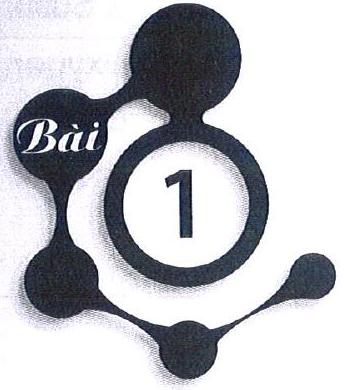
\includegraphics[max width=\textwidth, center]{2025_10_23_ae7aef68fb3b41082d29g-01}

\section*{KHÁI NIỆM}
VỀ CÂN BẦNG HOÁ HỌC

Dữ liệu áp dụng cho câu 1.1, 1.2, 1.3, 1.4 và 1.5.\\
Cho phương trình hoá học của phản ứng sản xuất ammonia trong công nghiệp:

$$
\mathrm{N}_{2}(g)+3 \mathrm{H}_{2}(g) \stackrel{380^{\circ} \mathrm{C}-450^{\circ} \mathrm{C}, 200 \mathrm{bar}, \mathrm{Fe}}{\rightleftharpoons} 2 \mathrm{NH}_{3}(g) \quad \Delta_{\mathrm{r}} \mathrm{H}_{298}^{\mathrm{o}}=-91,8 \mathrm{~kJ}
$$

1.1. Yếu tố nào không làm ảnh hưởng đến sự chuyển dịch cân bằng hoá học của phản ứng trên?\\
A. Nhiệt độ.\\
B. Nồng độ.\\
C. Áp suất.\\
D. Chất xúc tác.\\
1.2. Cân bằng hoá học sẽ chuyển dịch về phía tạo ra nhiều ammonia hơn khi\\
A. giảm nồng độ của khí nitrogen.\\
B. giảm nồng độ của khí hydrogen.\\
C. tăng nhiệt độ của hệ phản ứng.\\
D. tăng áp suất của hệ phản ứng.\\
1.3. Cân bằng hoá học sẽ chuyển dịch theo chiều nào khi\\
a) giảm nhiệt độ của hệ phản ứng?\\
b) tăng nồng độ của khí nitrogen?\\
c) tăng nồng độ của khí hydrogen?\\
d) giảm áp suất của hệ phản ứng?

Giải thích.\\
1.4. Viết biểu thức tính hằng số cân bằng $K_{\mathrm{C}}$ của phản ứng trên.\\
1.5. Khi tổng hợp $\mathrm{NH}_{3}$ từ $\mathrm{N}_{2}$ và $\mathrm{H}_{2}$ thấy rằng nồng độ ở trạng thái cân bằng của $\mathrm{N}_{2}$ là $0,02 \mathrm{M}$; của $\mathrm{H}_{2}$ là 2 M và của $\mathrm{NH}_{3}$ là $0,6 \mathrm{M}$. Tính hằng số cân bằng của phản ứng.

\section*{Dữ liệu dưng cho bài tập 1.6, 1.7, 1.8, 1.9, 1.10 và 1.11.}
Trong quy trình sản xuât sulfuric acid ( $\mathrm{H}_{2} \mathrm{SO}_{4}$ ) có giai đoạn dùng dung dịch $\mathrm{H}_{2} \mathrm{SO}_{4} 98 \%$ hấp thụ sulfur trioxide $\left(\mathrm{SO}_{3}\right)$ thu được oleum $\left(\mathrm{H}_{2} \mathrm{SO}_{4} \cdot \mathrm{nSO}_{3}\right)$. Sulfur trioxide được tạo thành bằng cách oxi hoá sulfur dioxide bằng oxygen hoặc lượng dư không khí ở nhiệt độ $450^{\circ} \mathrm{C}-500^{\circ} \mathrm{C}$, chất xúc tác vanadium (V) oxide $\left(\mathrm{V}_{2} \mathrm{O}_{5}\right)$ theo phương trình hoá học:

$$
2 \mathrm{SO}_{2}(g)+\mathrm{O}_{2}(g) \stackrel{\mathrm{V}_{2} \mathrm{O}_{5}, 450^{\circ} \mathrm{C}-500^{\circ} \mathrm{C}}{\rightleftharpoons} 2 \mathrm{SO}_{3}(g) \quad \Delta_{\mathrm{r}} \mathrm{H}_{298}^{\circ}=-198,4 \mathrm{~kJ}
$$

1.6. Cân bằng hoá học sẽ chuyển dịch theo chiều nào khi\\
a) tăng nhiệt độ của hệ phản ứng?\\
b) tăng nồng độ của khí $\mathrm{SO}_{2}$ ?\\
c) tăng nồng độ của khí $\mathrm{O}_{2}$ ?\\
d) dùng dung dịch $\mathrm{H}_{2} \mathrm{SO}_{4} 98 \%$ hấp thụ $\mathrm{SO}_{3}$ sinh ra?

Giải thích.\\
1.7. Viết biểu thức tính hằng số cân bằng $K_{c}$ của phản ứng trên.\\
1.8. Nồng độ ban đầu của $\mathrm{SO}_{2}$ và $\mathrm{O}_{2}$ tương ứng là 4 M và 2 M . Tính hằng số cân bằng của phản ứng, biết rằng khi đạt trạng thái cân bằng đã có $80 \% \mathrm{SO}_{2}$ đã phản ứng.\\
1.9. Để có $90 \% \mathrm{SO}_{2}$ đã phản ứng khi hệ đạt trạng thái cân bằng thì lúc đầu cần lấy lượng $\mathrm{O}_{2}$ là bao nhiêu? Biết nồng độ ban đầu của $\mathrm{SO}_{2}$ là 4 M .\\
1.10. Nếu tăng áp suất của hệ phản ứng và giữ nhiệt độ không đổi thì cân bằng của hệ sẽ chuyển dịch theo chiều nào?\\
1.11. Cho các biện pháp: (1) tăng nhiệt độ, (2) tăng áp suất chung của hệ phản ứng, (3) hạ nhiệt độ, (4) dùng thêm chất xúc tác $\mathrm{V}_{2} \mathrm{O}_{5}$, (5) giảm nồng độ $\mathrm{SO}_{3}$, (6) giảm áp suất chung của hệ phản ứng. Những biện pháp nào làm cân bằng trên chuyển dịch theo chiều thuận?\\
A. (1), (2), (4), (5).\\
B. (2), (3), (5).\\
C. (2), (3), (4), (6).\\
D. (1), (2), (4).\\
1.12. Khi hoà tan khí chlorine vào nước tạo thành dung dịch có màu vàng lục nhạt gọi là nước chlorine. Trong nước chlorine xảy ra cân bằng hoá học sau:

$$
\mathrm{Cl}_{2}+\mathrm{H}_{2} \mathrm{O} \rightleftharpoons \mathrm{HClO}+\mathrm{HCl}
$$

Acid HClO sinh ra không bền, dễ bị phân huỷ theo phản ứng:

$$
\mathrm{HClO} \rightarrow \mathrm{HCl}+\mathrm{O}
$$

Nước chlorine sẽ nhạt màu dần theo thời gian, không bảo quản được lâu. Vận dụng nguyên lí chuyển dịch cân bằng hoá học, hãy giải thích hiện tượng trên.\\
1.13. Hãy cho biết sự thay đổi áp suất có gây ra sự chuyển dịch cân bằng của mọi phản ứng thuận nghịch không. Giải thích.\\
1.14. Dựa vào giá trị hằng số cân bằng của các phản ứng dưới đây, hãy cho biết phản ứng nào có hiệu suất cao nhất và phản ứng nào có hiệu suất thấp nhất.\\
(a) $\mathrm{N}_{2} \mathrm{O}_{4}(g) \stackrel{10^{\circ} \mathrm{C}}{\rightleftharpoons} 2 \mathrm{NO}_{2}(g)$

$$
K_{\mathrm{c}}=0,2
$$

(b) $\mathrm{H}_{2}(g)+\mathrm{I}_{2}(g) \stackrel{450^{\circ} \mathrm{C}}{\rightleftharpoons} 2 \mathrm{HI}(g)$

$$
K_{\mathrm{c}}=50
$$

(c) $\mathrm{CO}_{2}(g)+\mathrm{H}_{2}(g) \stackrel{827^{\circ} \mathrm{C}}{\rightleftharpoons} \mathrm{CO}(g)+\mathrm{H}_{2} \mathrm{O}(g)$

$$
K_{\mathrm{C}}=0,659
$$

1.15. Cho vào bình kín (dung tích 1 L$) 1 \mathrm{~mol} \mathrm{H}_{2}$ và $1 \mathrm{~mol} \mathrm{I}_{2}$, sau đó thực hiện phản ứng ở $350^{\circ} \mathrm{C}-500^{\circ} \mathrm{C}$ theo phương trình hoá học sau:

$$
\mathrm{H}_{2}(g)+\mathrm{I}_{2}(g) \stackrel{350^{\circ} \mathrm{C}-500^{\circ} \mathrm{C}, \mathrm{Pt}}{\rightleftharpoons} 2 \mathrm{HI}(g)
$$

Ở trạng thái cân bằng thấy có sự tạo thành $1,56 \mathrm{~mol} \mathrm{HI}$. Tính hằng số cân bằng của phản ứng trên.\\
1.16. Bromine chloride phân huỷ tạo thành bromine và chlorine theo phương trình hoá học sau:

$$
2 \mathrm{BrCl}(g) \rightleftharpoons \mathrm{Br}_{2}(g)+\mathrm{Cl}_{2}(g)
$$

Ở nhiệt độ xác định, hằng số cân bằng của phản ứng trên có giá trị là 11,1 . Giả sử BrCl được cho vào vào bình kín có dung tích 1 L . Kết quả phân tích\\
cho biết hỗn hợp phản ứng ở trạng thái cân bằng có $4 \mathrm{~mol} \mathrm{Cl}_{2}$. Tính nồng độ mol của BrCl ở trạng thái cân bằng.\\
1.17*. Trong dung dịch muối $\mathrm{Fe}^{3+}$ tồn tại cân bằng hoá học sau:

$$
\mathrm{Fe}^{3+}+3 \mathrm{H}_{2} \mathrm{O} \rightleftharpoons \mathrm{Fe}(\mathrm{OH})_{3} \downarrow+3 \mathrm{H}^{+}
$$

Trong phòng thí nghiệm, để bảo quản dung dịch $\mathrm{Fe}^{3+}$, người ta thường thêm vào bình đựng vài giọt dung dịch acid HCl hoặc $\mathrm{H}_{2} \mathrm{SO}_{4}$ loãng. Giải thích.\\
1.18*. Phản ứng tổng hợp 3-methylbutyl acetate (isoamyl acetate) trong phòng thí nghiệm từ acetic acid và 3-methylbutan-1-ol (isoamyl alcohol) với xúc tác dung dịch $\mathrm{H}_{2} \mathrm{SO}_{4}$ đặc, đun nóng xảy ra theo phương trình hoá học sau:\\
$\mathrm{CH}_{3} \mathrm{COOH}+\left(\mathrm{CH}_{3}\right)_{2} \mathrm{CHCH}_{2} \mathrm{CH}_{2} \mathrm{OH} \xlongequal{\mathrm{H}_{2} \mathrm{SO}_{4} \text { đặc, to }} \mathrm{CH}_{3} \mathrm{COOCH}_{2} \mathrm{CH}_{2} \mathrm{CH}\left(\mathrm{CH}_{3}\right)_{2}+\mathrm{H}_{2} \mathrm{O}$\\
Ngoài vai trò là chất xúc tác, dung dịch $\mathrm{H}_{2} \mathrm{SO}_{4}$ đặc còn có vai trò gì trong việc nâng cao hiệu suất của phản ứng trên?\\
1.19*. Trong dung dịch muối $\mathrm{AlCl}_{3}$ tồn tại các cân bằng hoá học sau:


\begin{align*}
& \mathrm{Al}^{3+}+\mathrm{H}_{2} \mathrm{O} \rightleftharpoons \mathrm{Al}(\mathrm{OH})^{2+}+\mathrm{H}^{+}  \tag{1}\\
& \mathrm{Al}(\mathrm{OH})^{2+}+\mathrm{H}_{2} \mathrm{O} \rightleftharpoons \mathrm{Al}(\mathrm{OH})_{2}^{+}+\mathrm{H}^{+}  \tag{2}\\
& \mathrm{Al}(\mathrm{OH})_{2}^{+}+\mathrm{H}_{2} \mathrm{O} \rightleftharpoons \mathrm{Al}(\mathrm{OH})_{3} \downarrow+\mathrm{H}^{+} \tag{3}
\end{align*}


Khi thêm hỗn hợp $\mathrm{KIO}_{3}$ và KI vào dung dịch $\mathrm{AlCl}_{3}$ thì xảy ra phản ứng:


\begin{equation*}
\mathrm{KIO}_{3}+5 \mathrm{KI}+6 \mathrm{H}^{+} \rightarrow 3 \mathrm{I}_{2}+6 \mathrm{~K}^{+}+3 \mathrm{H}_{2} \mathrm{O} \tag{4}
\end{equation*}


Hãy giải thích sự xuất hiện kết tủa keo trắng trong thí nghiệm trên.\\
1.20*. Theo báo cáo mới nhất vừa được Ủy ban Liên chính phủ về Biến đổi khí hậu (IPCC) công bố ngày 09/8/2021, lượng khí thải gây hiệu ứng nhà kính do các hoạt động của con người là nguyên nhân chính gây ra hiện tượng ấm lên khoảng $1,1^{\circ} \mathrm{C}$ của Trái Đất trong khoảng thời gian từ năm 1850 1900. Hãy giải thích vì sao dù lượng khí $\mathrm{CO}_{2}$ thải ra từ các hoạt động công nghiệp hằng năm rất lớn nhưng nồng độ của chất khí này trong khí quyển lại tăng chậm.

Brit\\
2

\section*{CÂN BẰNG TRONG DUNG DICH NUỚC}
2.1. Vì sao dung dịch của các muối, acid, base dẫn điện?\\
A. Do có sự di chuyển của electron tạo thành dòng electron.\\
B. Do phân tử của chúng dẫn được điện.\\
C. Do các ion hợp phần có khả năng dẫn điện.\\
D. Do muối, acid, base có khả năng phân li ra ion trong dung dịch.\\
2.2. Dung dịch sodium chloride $(\mathrm{NaCl})$ dẫn được điện là do\\
A. NaCl tan được trong nước.\\
B. NaCl điện li trong nước thành ion.\\
C. NaCl có vị mặn.\\
D. NaCl là phân tử phân cực.\\
2.3. Saccharose là chất không điện li vì\\
A. phân tử saccharose không có khả năng hoà tan trong nước.\\
B. phân tử saccharose không có khả năng phân li thành ion trong nước.\\
C. phân tử saccharose không có tính dẫn điện.\\
D. phân tử saccharose có khả năng hoà tan trong nước.\\
2.4. Phát biểu nào sau đây đúng khi nói về sự điện li?\\
A. Sự điện li là quá trình phân li một chất trong nước thành ion.\\
B. Sự điện li quá trình hoà tan một chất vào nước tạo thành dung dịch.\\
C. Sự điện li là quá trình phân li một chất dưới tác dụng của dòng điện.\\
D. Sự điện li thực chất là quá trình oxi hoá - khử.\\
2.5. Các chất trong dãy nào sau đây là những chất điện li mạnh?\\
A. $\mathrm{HCl}, \mathrm{NaOH}, \mathrm{CH}_{3} \mathrm{COOH}$.\\
B. $\mathrm{KOH}, \mathrm{NaCl}, \mathrm{H}_{3} \mathrm{PO}_{4}$.\\
C. $\mathrm{HCl}, \mathrm{NaOH}, \mathrm{NaCl}$.\\
D. $\mathrm{NaNO}_{3}, \mathrm{NaNO}_{2}, \mathrm{NH}_{3}$.\\
2.6. Phương trình điện li nào sau đây biểu diễn không đúng?\\
A. $\mathrm{HF} \rightarrow \mathrm{H}^{+}+\mathrm{F}^{-}$\\
B. $\mathrm{CH}_{3} \mathrm{COOH} \rightleftharpoons \mathrm{CH}_{3} \mathrm{COO}^{-}+\mathrm{H}^{+}$\\
C. $\mathrm{NaCl} \rightarrow \mathrm{Na}^{+}+\mathrm{Cl}^{-}$\\
D. $\mathrm{NaOH} \rightarrow \mathrm{Na}^{+}+\mathrm{OH}^{-}$\\
2.7. Phương trình điện li nào sau đây biểu diễn đúng?\\
A. $\mathrm{NaOH} \rightleftharpoons \mathrm{Na}^{+}+\mathrm{OH}^{-}$\\
B. $\mathrm{HClO} \rightarrow \mathrm{H}^{+}+\mathrm{ClO}^{-}$\\
C. $\mathrm{Al}_{2}\left(\mathrm{SO}_{4}\right)_{3} \rightarrow 2 \mathrm{Al}^{3+}+3 \mathrm{SO}_{4}^{2-}$\\
D. $\mathrm{NH}_{4} \mathrm{Cl} \rightleftharpoons \mathrm{NH}_{4}^{+}+\mathrm{Cl}^{-}$\\
2.8. Khi chuẩn độ, người ta thêm từ từ dung dịch đựng trong (1) ... vào dung dịch đựng trong bình tam giác. Dụng cụ cần điền vào (1) là\\
A. bình định mức.\\
B. burette.\\
C. pipette.\\
D. ống đong.\\
2.9. Cho các chất sau: glucose $\left(\mathrm{C}_{6} \mathrm{H}_{12} \mathrm{O}_{6}\right), \mathrm{NaCl}, \mathrm{KOH}, \mathrm{Ba}(\mathrm{OH})_{2}, \mathrm{AlCl}_{3}, \mathrm{CuSO}_{4}$, $\mathrm{N}_{2}, \mathrm{O}_{2}, \mathrm{H}_{2} \mathrm{SO}_{4}$, saccharose ( $\mathrm{C}_{12} \mathrm{H}_{22} \mathrm{O}_{11}$ ).\\
Chất nào là chất điện li trong các chất trên?\\
2.10. Viết phương trình điện li của các chất sau trong nưởc: $\mathrm{HBr}, \mathrm{HNO}_{3}, \mathrm{KOH}$, $\mathrm{Ca}(\mathrm{OH})_{2}, \mathrm{Al}_{2}\left(\mathrm{SO}_{4}\right)_{3}, \mathrm{Cu}\left(\mathrm{NO}_{3}\right)_{2}$, Nal, HCN, HF, HCOOH.\\
2.11. Tính nồng độ mol của các ion trong các dung dịch sau:\\
a) $\mathrm{Ba}\left(\mathrm{NO}_{3}\right)_{2} 0,1 \mathrm{M}$.\\
b) $\mathrm{HNO}_{3} 0,02 \mathrm{M}$.\\
c) $\mathrm{KOH} 0,01 \mathrm{M}$.\\
2.12. Khả năng dẫn điện của nước vôi trong (dung dịch $\mathrm{Ca}(\mathrm{OH})_{2}$ trong nước) để trong không khí giảm dần theo thời gian. Hãy giải thích điều này.\\
2.13. Trong các phản ứng dưới đây, hãy cho biết ở phản ứng nào nước đóng vai trò là acid, ở phản ứng nào nước đóng vai trò là base theo thuyết Brønsted - Lowry:\\
a) $\mathrm{HCl}+\mathrm{H}_{2} \mathrm{O} \rightarrow \mathrm{H}_{3} \mathrm{O}^{+}+\mathrm{Cl}^{-}$\\
b) $\mathrm{NH}_{3}+\mathrm{H}_{2} \mathrm{O} \rightleftharpoons \mathrm{NH}_{4}^{+}+\mathrm{OH}^{-}$\\
c) $\mathrm{CH}_{3} \mathrm{COOH}+\mathrm{H}_{2} \mathrm{O} \rightleftharpoons \mathrm{H}_{3} \mathrm{O}^{+}+\mathrm{CH}_{3} \mathrm{COO}^{-}$\\
d) $\mathrm{CO}_{3}^{2-}+\mathrm{H}_{2} \mathrm{O} \rightleftharpoons \mathrm{HCO}_{3}^{-}+\mathrm{OH}^{-}$\\
2.14. Cho các phân tử và ion sau: $\mathrm{HI}, \mathrm{CH}_{3} \mathrm{COO}^{-}, \mathrm{H}_{2} \mathrm{PO}_{4}^{-}, \mathrm{PO}_{4}^{3-}, \mathrm{NH}_{3}, \mathrm{~S}^{2-}, \mathrm{HPO}_{4}^{2-}$. Hãy cho biết phân tử, ion nào là acid, base, lưỡng tính theo thuyết Brønsted Lowry. Giải thích.\\
2.15. a) Tính pH của dung dịch có nồng độ ion $\mathrm{H}^{+}$là $4,2 \times 10^{-10} \mathrm{M}$.\\
b) Tính nồng độ mol của ion $\mathrm{H}^{+}$trong dung dịch có $\mathrm{pH}=6,35$.\\
c) Tính pH của dung dịch có nồng độ ion $\mathrm{OH}^{-}$là $4,0 \times 10^{-11} \mathrm{M}$.\\
2.16. Cho 10 mL dung dịch HCl có $\mathrm{pH}=3$. Hãy đề nghị cách pha dung dịch có $\mathrm{pH}=4$ từ dung dịch trên.\\
2.17. Vì sao người ta không sử dụng dung dịch acid $\mathrm{HNO}_{3}$ trong phương pháp chuẩn độ acid - base?\\
2.18. Trộn 3 dung dịch $\mathrm{H}_{2} \mathrm{SO}_{4} 0,1 \mathrm{M}, \mathrm{HNO}_{3} 0,2 \mathrm{M}$ và $\mathrm{HCl} 0,3 \mathrm{M}$ với thể tích bằng nhau thu được dung dịch (A). Lấy 300 mL dung dịch (A) cho tác dụng với một dung dịch (B) gồm $\mathrm{NaOH} 0,20 \mathrm{M}$ và $\mathrm{KOH} 0,29 \mathrm{M}$. Tính thể tích dung dịch (B) cần dùng để sau khi tác dụng với 300 mL dung dịch (A) thu được dung dịch có $\mathrm{pH}=2$.\\
2.19. Để chuẩn độ 40 mL dung dịch HCl chưa biết nồng độ đã dùng trung bình hết 34 mL dung dịch $\mathrm{NaOH} 0,12 \mathrm{M}$. Tính nồng độ mol của dung dịch HCl .\\
2.20. Để chuẩn độ 50 mL dung dịch $\mathrm{CH}_{3} \mathrm{COOH}$ chưa biết nồng độ đã dùng trung bình hết 75 mL dung dịch $\mathrm{NaOH} 0,05 \mathrm{M}$. Tính nồng độ mol của dung dịch $\mathrm{CH}_{3} \mathrm{COOH}$.\\
2.21*. Trong phương pháp chuẩn độ acid - base, xung quanh điểm tương đương có một sự thay đổi pH đột ngột gọi là bước nhảy chuẩn độ. Đường biểu diễn trên đồ thị chuẩn độ acid - base gọi là đường định phân.\\
Từ các số liệu sau đây, hãy vẽ đồ thị biểu diễn sự biến thiên pH của dung dịch trong quá trình chuẩn độ dung dịch HCl bằng dung dịch chuẩn $\mathrm{NaOH} 0,100 \mathrm{M}$. Trục hoành ghi thể tích dung dịch NaOH , trục tung ghi pH của dung dịch. Xác định giá trị điểm tương đương và khoảng bước nhảy chuẩn độ của quá trình này.

\begin{center}
\begin{tabular}{|l|l|l|l|}
\hline
$\mathrm{V}_{\text {NaOH }}(\mathrm{mL})$ & Giá trị pH & $\mathrm{V}_{\text {Nao⿴囗 }}(\mathrm{mL})$ & Giá trị pH \\
\hline
0,0 & 1,00 & 25,1 & 10,30 \\
\hline
5,0 & 1,18 & 25,5 & 11,00 \\
\hline
10,0 & 1,37 & 26,0 & 11,29 \\
\hline
15,0 & 1,60 & 28,0 & 11,75 \\
\hline
20,0 & 1,95 & 30,0 & 11,96 \\
\hline
22,0 & 2,20 & 35,0 & 12,22 \\
\hline
24,0 & 2,69 & 40,0 & 12,36 \\
\hline
24,5 & 3,00 & 45,0 & 12,46 \\
\hline
24,9 & 3,70 & 50,0 & 12,52 \\
\hline
25,0 & 7,00 &  &  \\
\hline
\end{tabular}
\end{center}

\section*{ÔN TẬP CHƯONG 1}
Dữ liệu áp dụng cho câu OT1.1, OT1.2.\\
Cho phương trình nhiệt hoá học sau:\\
$\mathrm{C}_{2} \mathrm{H}_{2}(\mathrm{~g})+\mathrm{H}_{2} \mathrm{O}(\mathrm{g}) \stackrel{\mathrm{t}^{\circ}, \mathrm{xt}}{\rightleftharpoons} \mathrm{CH}_{3} \mathrm{CHO}(\mathrm{g}) \quad \Delta_{\mathrm{r}} \mathrm{H}_{298}^{\mathrm{o}}=-151 \mathrm{~kJ}$\\
OT1.1. Cân bằng hoá học sẽ chuyển dịch về phía tạo ra nhiều $\mathrm{CH}_{3} \mathrm{CHO}$ hơn khi\\
A. giảm nồng độ của khí $\mathrm{C}_{2} \mathrm{H}_{2}$.\\
B. tăng nhiệt độ của hệ phản ứng.\\
C. không sử dụng chất xúc tác.\\
D. tăng áp suất của hệ phản ứng.

OT1.2. Biểu thức tính hằng số cân bằng $K_{\mathrm{c}}$ của phản ứng là\\
A. $K_{\mathrm{C}}=\frac{\left[\mathrm{C}_{2} \mathrm{H}_{2}\right] \times\left[\mathrm{H}_{2} \mathrm{O}\right]}{\left[\mathrm{CH}_{3} \mathrm{CHO}\right]}$\\
B. $K_{\mathrm{C}}=\frac{\left[\mathrm{CH}_{3} \mathrm{CHO}\right]}{\left[\mathrm{C}_{2} \mathrm{H}_{2}\right] \times\left[\mathrm{H}_{2} \mathrm{O}\right]}$\\
C. $K_{C}=\frac{\left[\mathrm{C}_{2} \mathrm{H}_{2}\right]}{\left[\mathrm{CH}_{3} \mathrm{CHO}\right]}$\\
D. $K_{\mathrm{C}}=\frac{\left[\mathrm{CH}_{3} \mathrm{CHO}\right]}{\left[\mathrm{C}_{2} \mathrm{H}_{2}\right]}$

OT1.3. Chất nào sau đây không phải chất điện li?\\
A. NaCl .\\
B. $\mathrm{C}_{6} \mathrm{H}_{12} \mathrm{O}_{6}$.\\
C. $\mathrm{HNO}_{3}$.\\
D. NaOH .

OT1.4. Phương trình điện li nào sau đây không chính xác?\\
A. $\mathrm{KCl} \rightleftharpoons \mathrm{K}^{+}+\mathrm{Cl}^{-}$\\
B. $\mathrm{HCOOH} \rightleftharpoons \mathrm{HCOO}^{-}+\mathrm{H}^{+}$\\
C. $\mathrm{HClO} \rightleftharpoons \mathrm{H}^{+}+\mathrm{ClO}^{-}$\\
D. $\mathrm{Ca}(\mathrm{OH})_{2} \rightarrow \mathrm{Ca}^{2+}+2 \mathrm{OH}^{-}$

OT1.5. Theo thuyết Brønsted - Lowry, $\mathrm{H}_{2} \mathrm{O}$ đóng vai trò gì trong phản ứng sau?

$$
\mathrm{S}^{2-}+\mathrm{H}_{2} \mathrm{O} \rightleftharpoons \mathrm{HS}^{-}+\mathrm{OH}^{-}
$$

A. Chất oxi hoá.\\
B. Chất khử.\\
C. Acid.\\
D. Base.

Dữ liệu áp dụng cho câu OT1.6, OT1.7.\\
Cho phản ứng: $\mathrm{CO}(g)+3 \mathrm{H}_{2}(g) \rightleftharpoons \mathrm{CH}_{4}(g)+\mathrm{H}_{2} \mathrm{O}(g)$\\
OT1.6. Nồng độ ở trạng thái cân bằng: $[\mathrm{CO}]=0,0613 \mathrm{~mol} / \mathrm{L} ;\left[\mathrm{H}_{2}\right]=0,1839 \mathrm{mol} / \mathrm{L},\left[\mathrm{CH}_{4}\right]=0,0387 \mathrm{~mol} / \mathrm{L}$ và $\left[\mathrm{H}_{2} \mathrm{O}\right]=0,0387 \mathrm{~mol} / \mathrm{L}$. Tính hằng số cân bằng của phản ứng.

OT1.7. Cân bằng của phản ứng sẽ chuyển dịch theo chiều nào khi:\\
a) Bơm thêm $\mathrm{H}_{2}$ vào hệ phản ứng?\\
b) Giảm áp suất?

OT1.8. Phản ứng:\\
$\mathrm{COCl}_{2}(g) \rightleftharpoons \mathrm{CO}(g)+\mathrm{Cl}_{2}(g)$ đạt trạng thái cân bằng ở 900 K .\\
Hằng số cân bằng của phản ứng có giá trị là $8,2 \times 10^{-2}$. Giả sử nồng độ mol ở trạng thái cân bằng của CO và $\mathrm{Cl}_{2}$ là $0,150 \mathrm{M}$. Tính nồng độ mol ở trạng thái cân bằng của $\mathrm{COCl}_{2}$.

OT1.9. Viết phương trình điện li (nếu có) của các chất trong dung dịch: KBr , $\mathrm{NO}_{2}, \mathrm{Ca}\left(\mathrm{NO}_{3}\right)_{2}, \mathrm{NaOH}, \mathrm{CH}_{4}, \mathrm{Ba}(\mathrm{OH})_{2}, \mathrm{Fe}_{2}\left(\mathrm{SO}_{4}\right)_{3}, \mathrm{Zn}\left(\mathrm{NO}_{3}\right)_{2}, \mathrm{KI}, \mathrm{H}_{2} \mathrm{~S}$, $\mathrm{CH}_{2}=\mathrm{CH}-\mathrm{COOH}, \mathrm{CuO}$.

OT1.10. Trộn lẫn V mL dung dịch $\mathrm{NaOH} 0,01 \mathrm{M}$ với V mL dung dịch $\mathrm{HCl} 0,03 \mathrm{M}$ thu được 2 V mL dung dịch Y . Tính pH của dung dịch Y .

\section*{Chuong 2. NLLROESIN VA SULFUR}
\section*{Biii}
\section*{3}
\section*{ĐƠN CHẤT NITROGEN}
3.1. Ở trạng thái tự nhiên, nitrogen\\
A. tồn tại ở dạng đơn chất và hợp chất.\\
B. chỉ tồn tại ở dạng đơn chất.\\
C. chỉ tồn tại ở dạng hợp chất.\\
D. tự do chiếm khoảng $20 \%$ thể tích không khí.\\
3.2. Cấu hình electron nguyên tử của nitrogen là\\
A. $1 s^{2} 2 s^{2} 2 p^{1}$.\\
B. $1 s^{2} 2 s^{2} 2 p^{5}$.\\
C. $1 s^{2} 2 s^{2} 2 p^{4}$.\\
D. $1 s^{2} 2 s^{2} 2 p^{3}$.\\
3.3. Tính chất nào sau đây của nitrogen không đúng?\\
A. Ơ' điều kiện thường, nitrogen là chất khí.\\
B. Nitrogen tan rất ít trong nước.\\
C. Nitrogen không duy trì sự cháy và sự hô hấp.\\
D. Nitrogen nặng hơn không khí.\\
3.4. Nitrogen trong không khí có vai trò nào sau đây?\\
A. Cung cấp đạm tự nhiên cho cây trồng.\\
B. Hình thành sấm sét.\\
C. Tham gia quá trình quang hợp của cây.\\
D. Tham gia hình thành mây.\\
3.5. a) Tại sao nitrogen là phi kim mạnh lại tồn tại được trong tự nhiên dưới dạng tự do?\\
b) Tại sao nitrogen phản ứng được với nhiều kim loại, nhưng trong vỏ Trái Đất không gặp một nitride ( $\mathrm{N}^{3-}$ ) kim loại nào cả?\\
3.6. Viết phản ứng chứng minh nitrogen hoạt động hoá học ở nhiệt độ cao.\\
3.7. Một bình kín có dung tích là $0,5 \mathrm{~L}$ chứa $1,5 \mathrm{~mol} \mathrm{H}_{2}$ và $0,5 \mathrm{~mol} \mathrm{~N}_{2}$ ở nhiệt độ xác định. Ở trạng thái cân bằng có $0,2 \mathrm{~mol} \mathrm{NH}_{3}$ tạo thành. Tính hằng số cân bằng $K_{\mathrm{C}}$ của phản ứng xảy ra trong bình.\\
3.8*. Tại sao ở điều kiện thường ( $25^{\circ} \mathrm{C}, 1$ bar), nitrogen tồn tại ở dạng phân tử $\mathrm{N}_{2}$ trong khi đó phosphorus lại tồn tại ở dạng $\mathrm{P}_{4}$ mà không xảy ra trường hợp ngược lại? Biết:

\begin{itemize}
  \item Năng lượng liên kết ba $\mathrm{N} \equiv \mathrm{N}$ là $941 \mathrm{~kJ} / \mathrm{mol}$.
  \item Năng lượng liên kết ba $\mathrm{P} \equiv \mathrm{P}$ là $490 \mathrm{~kJ} / \mathrm{mol}$.
  \item Năng lượng liên kết đơn N-N là $160 \mathrm{~kJ} / \mathrm{mol}$.
  \item Năng lượng liên kêt đơn P-P là $209 \mathrm{~kJ} / \mathrm{mol}^{(*)}$.\\
3.9. Xác định cụm từ phù hợp trong các ô từ (1) đến (7) để hoàn thành chu trình của nitrogen trong tự nhiên.\\
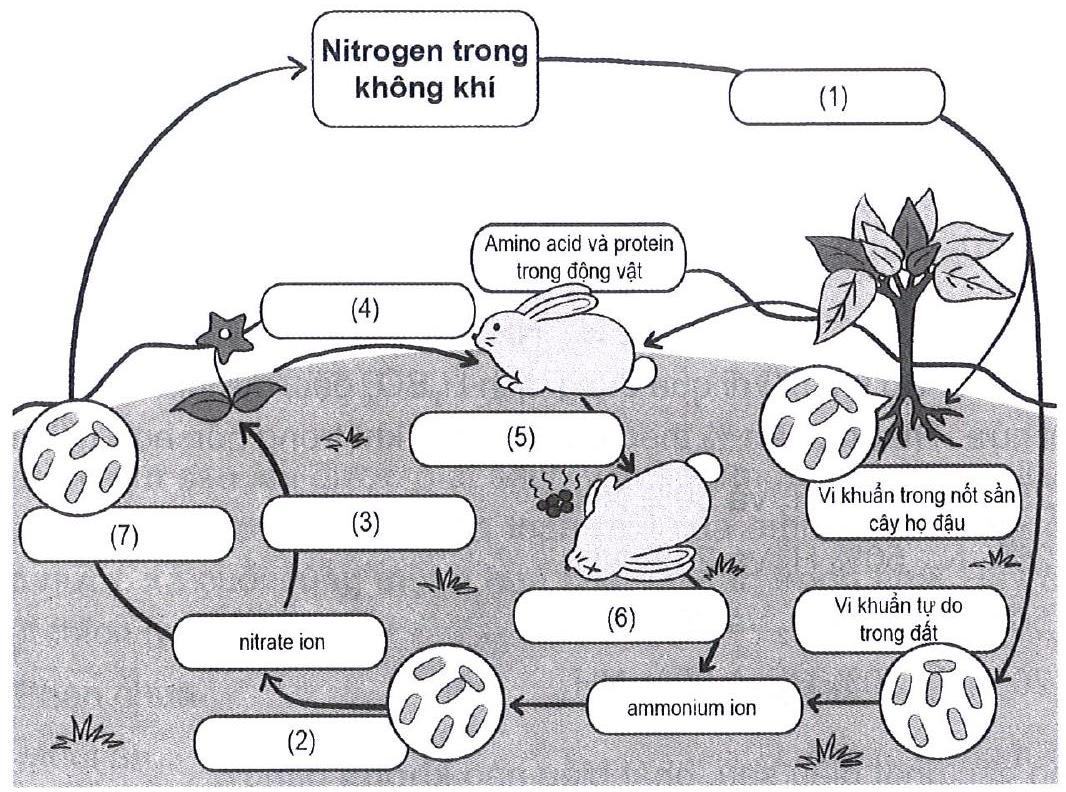
\includegraphics[max width=\textwidth, center]{2025_10_23_ae7aef68fb3b41082d29g-06}
\end{itemize}

\footnotetext{${ }^{(*)}$ Nguồn: \href{http://butane.chem.uiuc.edu/cyerkes/Chem104ACSpring2009/Genchemref/bondenergies.html}{http://butane.chem.uiuc.edu/cyerkes/Chem104ACSpring2009/Genchemref/bondenergies.html}
}
4.1. Liên kết trong phân tử $\mathrm{NH}_{3}$ là\\
A. liên kết cộng hoá trị phân cực.\\
B. liên kết ion.\\
C. liên kết cộng hoá trị không phân cực.\\
D. liên kết hydrogen.\\
4.2. Trong dung dịch, ammonia thể hiện tính base yếu do\\
A. phân tử ammonia chứa liên kết cộng hoá trị phân cực và liên kết hydrogen.\\
B. phân tử ammonia chứa liên kết cộng hoá trị phân cực và liên kết ion.\\
C. phần lớn các phân tử ammonia kết hợp với nước tạo ra các ion $\mathrm{NH}_{4}^{+}$và $\mathrm{OH}^{-}$.\\
D. một phần nhỏ các phân tử $\mathrm{NH}_{3}$ kết hợp với ion $\mathrm{H}^{+}$của nước tạo $\mathrm{NH}_{4}^{+}$và $\mathrm{OH}^{-}$.\\
4.3. Để tạo độ xốp cho một số loại bánh, có thể dùng chất nào sau đây?\\
A. $\left(\mathrm{NH}_{4}\right)_{3} \mathrm{PO}_{4}$.\\
B. $\mathrm{NH}_{4} \mathrm{HCO}_{3}$.\\
C. $\mathrm{CaCO}_{3}$.\\
D. NaCl .\\
4.4. Cho hỗn hợp khí ( X ) gồm $\mathrm{N}_{2}, \mathrm{H}_{2}, \mathrm{NH}_{3}$ có tỉ khối so với khí hydrogen là 8 . Dẫn hỗn hợp khí ( X ) đi qua dung dịch $\mathrm{H}_{2} \mathrm{SO}_{4}$ đặc, dư thì thể tích khí còn lại một nửa. Thành phần \% theo thể tích mỗi khí trong hỗn hợp $(X)$ lần lượt là\\
A. $25 \% \mathrm{~N}_{2}, 25 \% \mathrm{H}_{2}$ và $50 \% \mathrm{NH}_{3}$.\\
B. $25 \% \mathrm{~N}_{2}, 50 \% \mathrm{H}_{2}$ và $25 \% \mathrm{NH}_{3}$.\\
C. $50 \% \mathrm{~N}_{2}, 25 \% \mathrm{H}_{2}$ và $25 \% \mathrm{NH}_{3}$.\\
D. $20 \% \mathrm{~N}_{2}, 30 \% \mathrm{H}_{2}$ và $50 \% \mathrm{NH}_{3}$.\\
4.5. Trong các phát biểu sau, phát biểu nào không đúng?\\
A. Ở điều kiện thường, $\mathrm{NH}_{3}$ là chất khí không màu.\\
B. Khí $\mathrm{NH}_{3}$ nặng hơn không khí.\\
C. Khí $\mathrm{NH}_{3}$ dễ hoá lỏng, tan nhiều trong nước.\\
D. Phân tử $\mathrm{NH}_{3}$ chứa các liên kết cộng hoá trị phân cực.\\
4.6. Trong phòng thí nghiệm, người ta có thể phân biệt muối ammonium với một số muối khác bằng cách cho nó tác dụng với dung dịch base. Hiện tượng nào xảy ra?\\
A. Thoát ra một chất khí màu lục nhạt, làm xanh giấy quỳ tím ẩm.\\
B. Thoát ra một chất khi không màu, làm xanh giấy quỳ tím ẩm.\\
C. Thoát ra một chất khí màu nâu đỏ, làm xanh giấy quỳ tím ẩm.\\
D. Thoát ra một chất khí không màu, làm hồng giấy quỳ tím ẩm.\\
4.7. Trong các nhận xét dưới đây về muối ammonium, nhận xét nào đúng?\\
A. Muối ammonium tồn tại dưới dạng tinh thể ion, phân tử gồm cation ammonium và anion hydroxide.\\
B. Tất cả muối ammonium đều dễ tan trong nước, khi tan điện li hoàn toàn thành cation ammonium và anion gốc acid.\\
C. Dung dịch muối ammonium phản ứng với dung dịch base đặc, nóng thoát ra chất khí làm quỳ tím ẩm hoá đỏ.\\
D. Khi nhiệt phân các muối ammonium luôn có khí $\mathrm{NH}_{3}$ thoát ra.\\
4.8. Cho các phát biểu sau:\\
(1) Ammonia lỏng được dùng làm chất làm lạnh trong thiết bị lạnh.\\
(2) Để làm khô khí $\mathrm{NH}_{3}$ có lẫn hơi nước, có thể dẫn khí $\mathrm{NH}_{3}$ đi qua bình đựng dung dịch $\mathrm{H}_{2} \mathrm{SO}_{4}$ đặc.\\
(3) Khi cho quỳ tím ẩm vào lọ đựng khí $\mathrm{NH}_{3}$, quỳ tím chuyển thành màu đỏ.\\
(4) Nitrogen lỏng được dùng để bảo quản máu và các mẫu vật sinh học. Có bao nhiêu phát biểu đúng?\\
A. 2 .\\
B. 3.\\
C. 1.\\
D. 4.\\
4.9. Tã lót trẻ em sau khi được giặt sạch vẫn còn mùi khai do vẫn lưu lại một lượng ammonia. Để khử hoàn toàn mùi của ammonia thì người ta cho vào nước xả cuối cùng một ít hoá chất có sẵn trong nhà. Hãy chọn hoá chất thích hợp:\\
A. Phèn chua.\\
B. Giấm ăn.\\
C. Muối ăn.\\
D. Nước gừng tươi.\\
4.10. Trong khí thải của quy trình sản xuất thuốc trừ sâu, phân bón hoá học có lẫn khí $\mathrm{NH}_{3}$. Khí này rất độc đối với sức khoẻ của con người và gây ô nhiễm môi trường. Con người hít phải khí này với lượng lớn sẽ gây ngộ độc: ho, đau ngực (nặng), đau thắt ngực, khó thở, thở nhanh, thở khò khè; chảy nước mắt và bỏng mắt, mù mắt, đau họng nặng, đau miệng; mạch nhanh, yếu, sốc; lẫn lộn, đi lại khó khăn, chóng mặt, thiếu sự phối hợp, bồn chồn, ngẩn ngơ ${ }^{(*)}$. Để xử lí $\mathrm{NH}_{3}$ lẫn trong khí thải, người ta có thể dẫn khí thải

\footnotetext{${ }^{(7)}$ Nguồn: \href{http://nioeh.org.vn/vi/kham-va-phat-hien-benh-nghe-nghiep/nguy-co-nhiem-doc-amoniac-}{http://nioeh.org.vn/vi/kham-va-phat-hien-benh-nghe-nghiep/nguy-co-nhiem-doc-amoniac-}
}
trong moi-truong-lao-dong-va-cach-phong-tranh.html\\
qua một bể lọc chứa hoá chất nào sau đây?\\
A. Dung dịch $\mathrm{Ca}(\mathrm{OH})_{2}$.\\
B. Dung dịch HCl .\\
C. Dung dịch NaOH .\\
D. Nước.\\
4.11. Khi phun $\mathrm{NH}_{3}$ vào không khí bị nhiễm $\mathrm{Cl}_{2}$ thấy xuất hiện "khói trắng". Giải thích và viết phương trình hoá học minh hoạ.\\
4.12. Cho một ít chất chỉ thị phenolphtalein vào dung dịch $\mathrm{NH}_{3}$ loãng thu được dung dịch ( A ). Màu của dung dịch ( A ) thay đổi như thế nào khi\\
a) đun nóng dung dịch một hồi lâu.\\
b) thêm dung dịch HCl với số mol HCl bằng số mol $\mathrm{NH}_{3}$ có trong dung dịch (A).\\
c) thêm vài giọt dung dịch $\mathrm{Na}_{2} \mathrm{CO}_{3}$.\\
d) thêm từ từ dung dịch $\mathrm{AlCl}_{3}$ tới dư.\\
4.13. Xét phản ứng tổng hợp ammonia theo phương trình hoá học:
$$
\mathrm{N}_{2}(g)+3 \mathrm{H}_{2}(g) \rightleftharpoons \mathrm{t}^{\circ}, \mathrm{xt}, \mathrm{p} \rightleftharpoons 2 \mathrm{NH}_{3}(g)
$$

Ở nhiệt độ $T$, phản ứng đạt tới trạng thái cân bằng.\\
a) Cân bằng chuyển dịch theo chiều nào khi thêm $\mathrm{H}_{2}$ ? Khi thêm $\mathrm{NH}_{3}$ ?\\
b) Khi tăng thể tích của hệ thì cân bằng dịch chuyển như thế nào?\\
c) Giá trị của hằng số cân bằng thay đổi như thế nào trong trường hợp a) và trường hợp b)?\\
4.14*. Một lượng lớn ammonium ion trong nước rác thải sinh ra khi vứt bỏ vào ao hồ được vi khuẩn oxi hoá thành nitrate và quá trình đó làm giảm oxygen hoà tan trong nước gây ngạt cho sinh vật sống dưới nước. Người ta có thể xử lí nguồn gây ô nhiễm đó bằng nước vôi trong (dung dịch $\mathrm{Ca}(\mathrm{OH})_{2}$ ) và khí chlorine để chuyển ammonium ion thành ammonia rồi chuyển tiếp thành nitrogen không độc thải ra môi trường. Giải thích cách làm này bằng phương trình hoá học.\\
4.15. Muối $\mathrm{NH}_{4} \mathrm{NO}_{3}$ sẽ nhiệt phân theo phản ứng nào trong 2 phản ứng sau? Giải thích.


\begin{align*}
& \mathrm{NH}_{4} \mathrm{NO}_{3}(\mathrm{~s}) \xrightarrow{\mathrm{t}^{\circ}} \mathrm{NH}_{3}(\mathrm{~g})+\mathrm{HNO}_{3}(\mathrm{~g})  \tag{1}\\
& \mathrm{NH}_{4} \mathrm{NO}_{3}(\mathrm{~s}) \xrightarrow{\mathrm{t}^{\circ}} \mathrm{N}_{2} \mathrm{O}(\mathrm{~g})+2 \mathrm{H}_{2} \mathrm{O}(\mathrm{~g}) \tag{2}
\end{align*}


Biết enthalpy tạo thành chuẩn của các chất có giá trị như sau ${ }^{(*)}$ :

\begin{center}
\begin{tabular}{|c|c|c|c|c|c|}
\hline
Chất & $\mathrm{NH}_{4} \mathrm{NO}_{3}(\mathbf{s})$ & $\mathrm{NH}_{3}(\mathbf{g})$ & $\mathrm{N}_{2} \mathbf{O}(\mathbf{g})$ & $\mathrm{HNO}_{3}(\mathbf{g})$ & $\mathbf{H}_{2} \mathbf{O}(\mathbf{g})$ \\
\hline
$\Delta_{\mathrm{r}} \mathrm{H}_{298}^{\circ}(\mathrm{kJ} / \mathrm{mol})$ & $-365,61$ & $-45,90$ & 82,05 & $-134,31$ & $-241,82$ \\
\hline
\end{tabular}
\end{center}

4.16. Hiện nay người ta sản xuất ammonia bằng cách chuyển hoá có xúc tác một hỗn hợp gồm không khí, hơi nước và khí methane (thành phần chính của khí thiên nhiên).

Phản ứng điều chế $\mathrm{H}_{2}: \quad \mathrm{CH}_{4}+2 \mathrm{H}_{2} \mathrm{O} \stackrel{t^{\circ}, \mathrm{xt}}{\rightleftharpoons} \mathrm{CO}_{2}+4 \mathrm{H}_{2}$\\
Phản ứng loại $\mathrm{O}_{2}$ để thu $\mathrm{N}_{2}: \mathrm{CH}_{4}+2 \mathrm{O}_{2} \stackrel{t^{\circ}}{\longrightarrow} \mathrm{CO}_{2}+2 \mathrm{H}_{2} \mathrm{O}$

Phản ứng tổng hợp $\mathrm{NH}_{3}: \quad \mathrm{N}_{2}+3 \mathrm{H}_{2} \xlongequal{\mathrm{t}^{\circ}, \mathrm{xt}, \mathrm{p}} 2 \mathrm{NH}_{3}$

Để sản xuất khí ammonia, nếu lấy $841,7 \mathrm{~m}^{3}$ không khí (chựa $21,03 \% \mathrm{O} 78,02 \% \mathrm{~N}_{2}$, còn lại là khí hiếm theo thể tích), thì cần phải lấy bao nhiêu $\mathrm{m}^{3}$ khí methane và bao nhiêu $\mathrm{m}^{3}$ hơi nước để có đủ lượng $\mathrm{N}_{2}$ và $\mathrm{H}_{2}$ theo tỉ lệ $1: 3$ về thể tích dùng cho phản ứng tổng hợp ammonia. Giả thiết các phản ứng (1), (2) đều xảy ra hoàn toàn và các thể tích khí đo ở cùng điều kiện.\\
4.17. Hợp chất có công thức hoá học $\mathrm{NH}_{4} \mathrm{NO}_{3}$ được giới chức quốc gia Lebanon xác định là nguyên nhân gây ra vụ nổ thảm khốc ở thủ đô Beirut vào ngày 04/08/2020. Tia lửa hàn trong quá trình sửa chữa nhà kho có thể đã làm 2750 tấn $\mathrm{NH}_{4} \mathrm{NO}_{3}$ cất trữ phát nổ, phá huỷ nhiều nhà cửa, dẫn đến nhiều người thiệt mạng. Hãy giải thích vì sao $\mathrm{NH}_{4} \mathrm{NO}_{3}$ có khả năng phát nổ.

\footnotetext{${ }^{(*)}$ Nguồn: J. D. Cox, D. Harrop, A. J. Head, The standard enthalpy of formation of ammonium nitrate and of nitrate ion, J. Chem. Thermodynamic, 1979, Vol. 11, 811-814.
}\section*{Biii \\
 5}
\section*{MỘT SỐ HỢP CHẤT}
VỚI OXYGEN CỦA NITROGEN\\
5.1. Hiện tượng mưa acid\\
A. là hiện tượng sẵn có trong tự nhiên.\\
B. xảy ra do sự bốc hơi của nước rồi ngưng tụ.\\
C. xảy ra khi nước mưa có $\mathrm{pH}<7$.\\
D. xảy ra khi nước mưa có $\mathrm{pH}<5,6$.\\
5.2. Hiện tượng mưa acid là do không khí bị ô nhiễm bởi các khí nào sau đây?\\
A. $\mathrm{SO}_{2}, \mathrm{NO}, \mathrm{NO}_{2}$\\
B. $\mathrm{NO}, \mathrm{CO}, \mathrm{CO}_{2}$.\\
C. $\mathrm{CH}_{4}, \mathrm{HCl}, \mathrm{CO}$.\\
D. $\mathrm{Cl}_{2}, \mathrm{CH}_{4}, \mathrm{SO}_{2}$.\\
5.3. Cho phản ứng: $\mathrm{Fe}_{3} \mathrm{O}_{4}+\mathrm{HNO}_{3} \rightarrow \mathrm{Fe}\left(\mathrm{NO}_{3}\right)_{3}+\mathrm{NO} \uparrow+\mathrm{H}_{2} \mathrm{O}$

Hệ số tỉ lượng của $\mathrm{HNO}_{3}$ trong phương trình hoá học trên là\\
A. 4.\\
B. 1.\\
C. 28.\\
D. 10 .\\
5.4. Cho phản ứng: $\mathrm{aFe}+\mathrm{bHNO}_{3} \rightarrow \mathrm{cFe}\left(\mathrm{NO}_{3}\right)_{3}+\mathrm{dNO} \uparrow+\mathrm{eH}_{2} \mathrm{O}$

Hệ số tỉ lượng $\mathrm{a}, \mathrm{b}, \mathrm{c}, \mathrm{d}, \mathrm{e}$ là những số nguyên dương có tỉ lệ tối giản. Tổng $(\mathrm{a}+\mathrm{b})$ bằng\\
A. 3 .\\
B. 5 .\\
C. 4 .\\
D. 6 .\\
5.5. Phú dưỡng là hiện tượng xảy ra do sự gia tăng hàm lượng của nguyên tố nào trong nước?\\
A. Fe, Mn.\\
B. N, P.\\
C. $\mathrm{Ca}, \mathrm{Mg}$.\\
D. Cl, F.\\
5.6. Hãy đề xuất một số biện pháp làm giảm tác hại của mưa acid đối với đời sống của thực vật, vật nuôi và con người.\\
5.7. Giải thích vì sao người ta dùng chai có màu tối để chứa và bảo quản dung dịch nitric acid.\\
5.8. Sơ đồ quy trình dưới đây mô tả các bước trong quá trình sản xuất phân bón (Z). Hãy xác định các chất $(\mathrm{X}),(\mathrm{T}),(\mathrm{Y}),(\mathrm{Q}),(\mathrm{Z})$. Viết các phản ứng hoá học xảy ra.\\
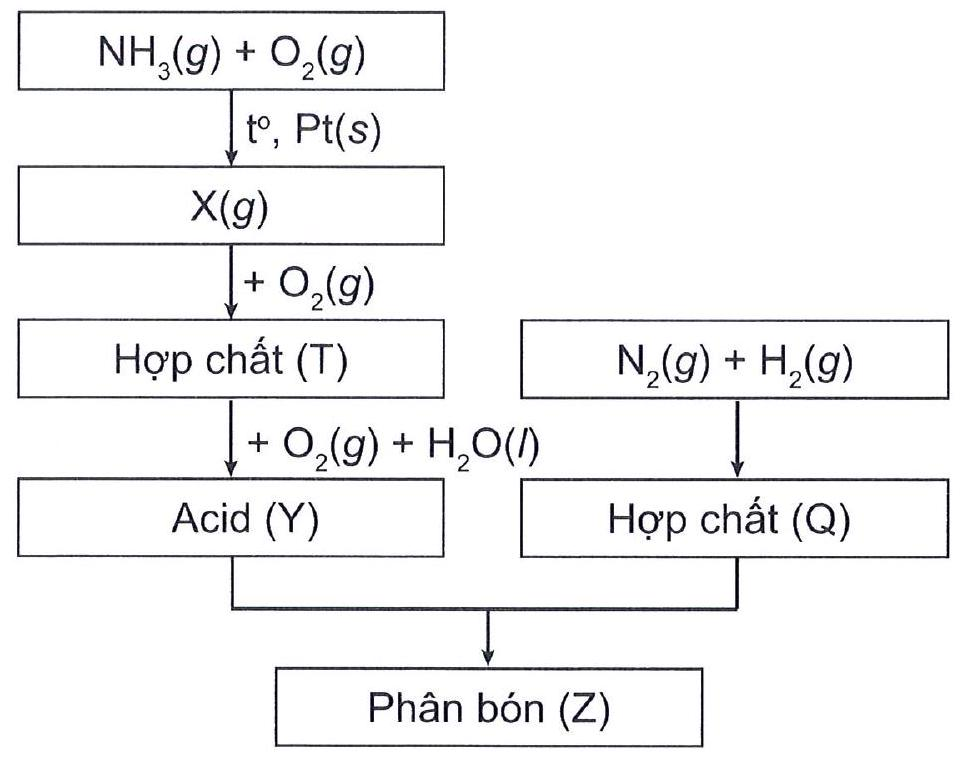
\includegraphics[max width=\textwidth, center]{2025_10_23_ae7aef68fb3b41082d29g-09}\\
5.9. Hãy sắp xếp theo đúng trình tự diễn biến quá trình hình thành hiện tượng phú dưỡng.

\begin{center}
\begin{tabular}{|l|c|}
\hline
\multicolumn{1}{|c|}{Tên quá trình} & Thứ tự \\
\hline
Thực vật chết. & $?$ \\
\hline
Thiếu oxygen. & $?$ \\
\hline
Thiếu ánh sáng mặt trời và oxygen nên tảo, thực vật và cá chết. & $?$ \\
\hline
\end{tabular}
\end{center}

\begin{center}
\begin{tabular}{|l|l|}
\hline
Vi khuẩn phát triển. & $?$ \\
\hline
Chất dinh dưỡng rửa trôi xuống ao, hồ. & $?$ \\
\hline
Tảo nở hoa và thực vật phát triển. & $?$ \\
\hline
\end{tabular}
\end{center}

5.10. Tính nồng độ $\mathrm{mol} / \mathrm{L}$ của dung dịch $\mathrm{HNO}_{3} 60 \%$, biết khối lượng riêng của dung dịch là $1,41 \mathrm{~g} / \mathrm{mL}$.\\
5.11. Sơ đồ phản ứng sau đây cho thấy rõ vai trò của thiên nhiên và con người trong việc vận chuyển nitrogen từ khí quyển vào trong đất, cung cấp nguồn phân đạm cho cây cối:

Hãy viết phương trình hoá học của các phản ứng trong sơ đồ chuyển hoá trên.\\
5.12*. Cho phương trình hoá học của phản ứng:

$$
\mathrm{N}_{2} \mathrm{O}_{4}(l)+2 \mathrm{~N}_{2} \mathrm{H}_{4}(l) \rightarrow 3 \mathrm{~N}_{2}(g)+4 \mathrm{H}_{2} \mathrm{O}(g)
$$

Biết enthalpy tạo thành chuẩn của các chất được trình bày trong bảng sau(*):

\begin{center}
\begin{tabular}{|c|c|c|c|}
\hline
Chất & $\mathbf{N}_{2} \mathbf{O}_{4} \boldsymbol{(} \boldsymbol{)}$ & $\mathbf{N}_{2} \mathbf{H}_{4} \boldsymbol{(} \boldsymbol{\mathrm { l }} \boldsymbol{)}$ & $\mathbf{H}_{2} \mathbf{O}(\mathbf{g})$ \\
\hline
$\Delta_{\mathrm{f}} \mathrm{H}_{298}^{\circ}(\mathrm{kJ} / \mathrm{mol})$ & $-19,56$ & 50,63 & $-241,82$ \\
\hline
\end{tabular}
\end{center}

a) Tính nhiệt đốt cháy 1 kg hỗn hợp lỏng gồm $\mathrm{N}_{2} \mathrm{O}_{4}$ và $\mathrm{N}_{2} \mathrm{H}_{4}$.\\
b) Tại sao hỗn hợp lỏng ( $\mathrm{N}_{2} \mathrm{O}_{4}$ và $\mathrm{N}_{2} \mathrm{H}_{4}$ ) được dùng làm nhiên liệu tên lửa?

\footnotetext{${ }^{(4)}$ Nguồn:\\
Martin S. Silberberg, Principles of General Chemistry (2013, third edition), The McGraw-Hill Companies, Inc., New York, USA.\\
\href{https://webbook.nist.gov/cgi/cbook.cgi?ID=C10544726&Mask=1E9F}{https://webbook.nist.gov/cgi/cbook.cgi?ID=C10544726\&Mask=1E9F}
}
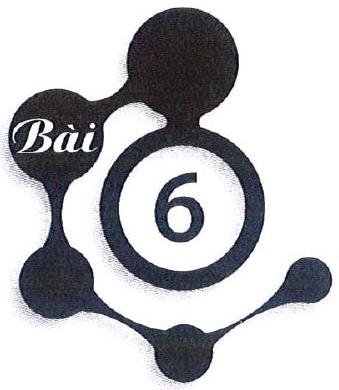
\includegraphics[max width=\textwidth, center]{2025_10_23_ae7aef68fb3b41082d29g-10}

\section*{SULFUR VÀ SULFUR DIOXIDE}
6.1. Phát biểu nào sau đây không đúng?\\
A. Lưu huỳnh là một nguyên tố phi kim, chỉ có tính oxi hoá.\\
B. Khi tham gia phản ứng, lưu huỳnh thể hiện tính oxi hoá hoặc tính khử.\\
C. Ở điều kiện thường, lưu huỳnh là chất rắn, màu vàng, không tan trong nước.\\
D. Ở điều kiện thường, lưu huỳnh tồn tại dạng phân tử tám nguyên tử ( $S_{8}$ ).\\
6.2. Cho các phản ứng hoá học sau:\\
(1) $\mathrm{S}+\mathrm{O}_{2} \rightarrow \mathrm{SO}_{2}$\\
(2) $\mathrm{S}+3 \mathrm{~F}_{2} \rightarrow \mathrm{SF}_{6}$\\
(3) $\mathrm{S}+\mathrm{Hg} \rightarrow \mathrm{HgS}$\\
(4) $\mathrm{S}+6 \mathrm{HNO}_{3}($ đặc $) \rightarrow \mathrm{H}_{2} \mathrm{SO}_{4}+6 \mathrm{NO}_{2} \uparrow+2 \mathrm{H}_{2} \mathrm{O}$

Trong các phản ứng trên, số phản ứng trong đó S thể hiện tính khử là\\
A. 3 .\\
B. 2.\\
C. 4.\\
D. 1.\\
6.3. Khí $\mathrm{SO}_{2}$ sinh ra từ việc đốt các nhiên liệu hoá thạch, các quặng sulfide là một trong các chất gây ô nhiễm môi trường, do $\mathrm{SO}_{2}$ góp phần gây ra\\
A. mưa acid.\\
B. hiện tượng khí nhà kính.\\
C. suy giảm tầng ozone.\\
D. nước thải gây ung thư.\\
6.4. Chất khí $(\mathrm{X})$ tan trong nước tạo ra dung dịch làm quỳ tím hoá đỏ và khí $(\mathrm{X})$ có thể được dùng làm chất tẩy màu. Khí $(\mathrm{X})$ là\\
A. $\mathrm{NH}_{3}$.\\
B. $\mathrm{CO}_{2}$.\\
C. $\mathrm{SO}_{2}$.\\
D. $\mathrm{O}_{3}$.\\
6.5. Cho các phương trình hoá học sau:\\
(1) $\mathrm{SO}_{2}+2 \mathrm{H}_{2} \mathrm{~S} \rightarrow 3 \mathrm{~S}+2 \mathrm{H}_{2} \mathrm{O}$\\
(2) $\mathrm{SO}_{2}+\mathrm{Br}_{2}+2 \mathrm{H}_{2} \mathrm{O} \rightarrow 2 \mathrm{HBr}+\mathrm{H}_{2} \mathrm{SO}_{4}$

Phát biểu nào sau đây đúng?\\
A. $\mathrm{SO}_{2}$ chỉ thể hiện tính oxi hoá.\\
B. $\mathrm{SO}_{2}$ chỉ thể hiện tính khử.\\
C. $\mathrm{SO}_{2}$ vừa thể hiện tính oxi hoá, vừa thể hiện tính khử.\\
D. $\mathrm{SO}_{2}$ không thể hiện tính khử và không thể hiện tính oxi hoá.\\
6.6. Hãy nêu phương pháp tách riêng bột lưu huỳnh và bột sắt ra khỏi hỗn hợp.\\
6.7. Hãy cho biết một phân tử lưu huỳnh ở trạng thái hơi $\left(900^{\circ} \mathrm{C}\right)$ gồm bao nhiêu nguyên tử, biết tỉ khối lưu huỳnh so với không khí ở $900^{\circ} \mathrm{C}$ bằng 2,207 . Từ đó nêu công thức phân tử của hơi lưu huỳnh ở $900^{\circ} \mathrm{C}$.\\
6.8. Lưu huỳnh có nhiều ứng dụng trong đời sông và sản xuất. Người ta dùng lưu huỳnh để bảo quản thuốc bắc cũng như bảo quản hoa quả tươi lâu hơn. Hãy giải thích điều này. Việc làm này có gây hại gì cho sức khoẻ con người không?\\
6.9. Lưu huỳnh là nguyên liệu quan trọng cho nhiều ngành công nghiệp như sản xuất $\mathrm{H}_{2} \mathrm{SO}_{4}$, lưu hoá cao su, chế tạo diêm, sản xuất chất tẩy trắng, ... Hãy cho biết trong tự nhiên có những nguồn cung cấp lưu huỳnh nào.\\
6.10. Thuỷ ngân là kim loại nặng rất độc. Việc con người tiếp xúc với thuỷ ngân trong thời gian dài dẫn đến run rẩy, mất khả năng điều hoà vận động, thay đổi tính cách, mất trí nhớ, mất ngủ, mệt mỏi, đau đầu, giảm cân, căng thẳng tâm lí và viêm lợi. Các triệu chứng này xảy ra khi một người tiếp xúc với nồng độ thuỷ ngân trong không khí trên $50 \mu \mathrm{~g} / \mathrm{m}^{3}{ }^{(4)}$. Thuỷ ngân độc hơn khi ở thể hơi vì dễ dàng hấp thụ vào cơ thể qua nhiều con đường như đường hô hấp, đường tiêu hoá, qua da, ... Trong trường hợp thuỷ ngân rơi vãi, cần xử lí như thế nào? Liên hệ với tình huống xử lí an toàn khi vô tình làm vỡ nhiệt kế thuỷ ngân trong phòng thí nghiệm.\\
6.11. Khí thải của các nhà máy, xí nghiệp, ... có chứa nhiều $\mathrm{SO}_{2}$. Đây là một trong những nguyên nhân chủ yếu gây ra mưa acid, gây tổn hại cho nhiều công trình làm bằng sắt, đá. Hãy giải thích bằng các phương trình hoá học xảy ra (nếu có).\\
6.12. Hãy cho biết người dân có thể đối mặt với những nguy cơ nào khi một nhà máy sản xuất lưu huỳnh bị cháy. Giải thích.\\
6.13*. Khi $\mathrm{SO}_{2}$ là một trong các chất chủ yếu gây ô nhiễm môi trường nhưng khi được sử dụng đúng mục đích sẽ có nhiều ứng dụng: dùng để sản xuất sulfuric acid, tẩy trắng giấy, bột giấy, chống nấm mốc cho lương thực, thực phẩm, ... Trong công nghiệp $\mathrm{SO}_{2}$ được sản xuất từ các nguyên liệu khác nhau như lưu huỳnh, đốt quặng pyrit sắt ( $\mathrm{FeS}_{2}$ ). Hãy cho biết ưu và nhược điểm đối với môi trường khi điều chế $\mathrm{SO}_{2}$ từ 2 loại nguyên liệu trên?

\footnotetext{(') Nguồn: \href{https://moh.gov.vn/web/phong-chong-benh-nghe-nghiep/thong-tin-hoat-dong/-/asset_publisher/}{https://moh.gov.vn/web/phong-chong-benh-nghe-nghiep/thong-tin-hoat-dong/-/asset\_publisher/} xjpQsFUZRw4q/content/nhiem-oc-thuy-ngan-nguy-hiem-the-nao-?inheritRedirect=false
}
6.14. Trái cây tươi cắt sẵn và đóng gói có thời hạn sử dụng ngắn. Sulfur dioxide thường được sử dụng để làm giảm sự thâm đen và sự phân huỷ, nhưng quá trình này gây nguy hiểm đến sức khoẻ của người tiêu dùng. Kĩ thuật đóng gói bổ sung khí (Modified Atmosphere Packaging - MAP) là một giải pháp an toàn thay thế. Hỗn hợp khí ở nhiệt độ thấp được sử dụng trong kĩ thuật MAP được trình bày như sau:

\begin{center}
\begin{tabular}{|l|c|c|}
\hline
\multicolumn{1}{|c|}{Sản phẩm} & $\mathbf{\% O}_{\mathbf{2}}$ (về thể tích) & $\mathbf{\% C O}_{\mathbf{2}}$ (về thể tích) \\
\hline
Táo & 4 & 2 \\
\hline
Dâu tây & 2,5 & 16 \\
\hline
Đậu Hà Lan & 9 & 7 \\
\hline
Cần tây & 11 & 9 \\
\hline
\end{tabular}
\end{center}

Bảng tổng hợp ở trên cho biết thành phần của hỗn hợp khí sử dụng đối với mỗi loại rau quả giúp chúng có thời hạn sử dụng lâu nhất. Khí còn lại là nitrogen.\\
a) Dựa vào bảng số liệu trên, hãy cho biết loại rau quả tươi nào ở trong bảng được đóng gói với hỗn hợp khí có thành phần $\mathrm{N}_{2}$ giống với không khí nhất?\\
A. Táo.\\
B. Dâu tây.\\
C. Đậu Hà Lan.\\
D. Cần tây.\\
b) Thực tế, do lợi ích kinh tế trước mắt mà nhiều tổ chức, cá nhân đã sử dụng hoá chất độc hại để bảo quản trái cây. Việc dùng hoá chất làm cho trái cây giữ được rất lâu. Những giải pháp bảo quản trái cây nào được cho là an toàn và không an toàn với người dùng? Đánh dấu $\checkmark$ vào bảng sau ở ô thích hợp.

\begin{center}
\begin{tabular}{|l|c|c|}
\hline
\multicolumn{1}{|c|}{Giải pháp} & An toàn & Không an toàn \\
\hline
(1) Dùng hoá chất $\mathrm{SO}_{2}$ để bảo quản trái cây. & $?$ & $?$ \\
\hline
(2) Bảo quản trái cây trong tủ lạnh. & $?$ & $?$ \\
\hline
(3) Kĩ thuật đóng gói bổ sung khí MAP. & $?$ & $?$ \\
\hline
\end{tabular}
\end{center}

\section*{SULFURIC ACID}
\section*{VÀ MUỐI SULFATE}
7.1. Kim loại nào sau đây không tác dụng với dung dịch $\mathrm{H}_{2} \mathrm{SO}_{4}$ loãng?\\
A. Al.\\
B. Zn.\\
C. Na.\\
D. Cu .\\
7.2. Dãy kim loại nào trong các dãy sau đây gồm các kim loại không tác dụng với dung dịch $\mathrm{H}_{2} \mathrm{SO}_{4}$ đặc, nguội?\\
A. $\mathrm{Al}, \mathrm{Fe}, \mathrm{Au}, \mathrm{Pt}$.\\
B. $\mathrm{Zn}, \mathrm{Pt}, \mathrm{Au}, \mathrm{Mg}$.\\
C. Al, Fe, Zn, Mg.\\
D. Al, $\mathrm{Fe}, \mathrm{Au}, \mathrm{Mg}$.\\
7.3. Dung dịch sulfuric acid đặc khác dung dịch sulfuric acid loãng ở tính chất hoá học nào?\\
A. Tính base mạnh.\\
B. Tính oxi hoá mạnh.\\
C. Tính acid mạnh.\\
D. Tính khử mạnh.\\
7.4. Cách pha loãng dung dịch $\mathrm{H}_{2} \mathrm{SO}_{4}$ đặc nào sau đây đúng?\\
A. Rót nhanh acid vào nước và khuấy đều.\\
B. Rót nhanh nước vào acid và khuấy đều.\\
C. Rót từ từ nước vào acid và khuấy đều.\\
D. Rót từ từ acid vào nước và khuây đều.\\
7.5. Người ta thường dùng các bình bằng thép đế đựng và chuyên chở dung dịch $\mathrm{H}_{2} \mathrm{SO}_{4}$ đặc vì\\
A. dung dịch $\mathrm{H}_{2} \mathrm{SO}_{4}$ đặc bị thụ động hoá trong thép.\\
B. dung dịch $\mathrm{H}_{2} \mathrm{SO}_{4}$ đặc không phản ứng với sắt ở nhiệt độ thường.\\
C. dung dịch $\mathrm{H}_{2} \mathrm{SO}_{4}$ đặc không phản ứng với kim loại ở nhiệt độ thường.\\
D. thép có chứa các chất phụ trợ không phản ứng với dung dịch $\mathrm{H}_{2} \mathrm{SO}_{4}$ đặc.\\
7.6. Hỗn hợp $(\mathrm{X})$ gồm Mg và $\mathrm{Fe}_{2} \mathrm{O}_{3}$ có khối lượng 20 gam tan hết trong dung dịch $\mathrm{H}_{2} \mathrm{SO}_{4}$ loãng thoát ra a L khí $\mathrm{H}_{2}(\mathrm{đkc})$ và tạo thành dung dịch $(\mathrm{Y})$. Thêm dung dịch NaOH dư vào dung dịch ( Y ) và lọc kết tủa, tách ra nung đến khối lượng không đổi thu được 28 gam chất rắn. Phần trăm khối lượng Mg trong hỗn hợp $(X)$ là\\
A. $40 \%$.\\
B. $60 \%$.\\
C. $25 \%$.\\
D. $75 \%$.\\
7.7. Bình đựng dung dịch $\mathrm{H}_{2} \mathrm{SO}_{4}$ đặc để trong không khí ẩm lâu ngày thì khối lượng bình có thay đổi không? Vì sao?\\
7.8. Trong lúc làm thí nghiệm, do bất cẩn nên một học sinh bị dung dịch $\mathrm{H}_{2} \mathrm{SO}_{4}$ đặc rơi lên tay. Hãy nêu biện pháp xử lí trong tình huống này trước khi đưa học sinh đến cơ sở y tế gần nhất.\\
7.9. Sulfuric acid là hoá chất hàng đầu trong nhiều ngành sản xuất, được mệnh danh là "máu" của các ngành công nghiệp. Trong công nghiệp, sulfuric acid được sản xuất bằng phương pháp tiếp xúc. Phương pháp này gồm 3 công đoạn chính: sản xuất $\mathrm{SO}_{2} \rightarrow$ sản xuất $\mathrm{SO}_{3} \rightarrow$ sản xuất $\mathrm{H}_{2} \mathrm{SO}_{4}$. Trong công đoạn sản xuất $\mathrm{SO}_{3}$ từ $\mathrm{SO}_{2}$ để thực hiện cần có điều kiện phản ứng thích hợp. Hãy cho biết điều kiện của phản ứng trên là gì? Biết rằng trong tự nhiên cũng có một lượng sulfuric acid sinh ra theo các công đoạn trên. Hãy giải thích quá trình hình thành.\\
7.10. Sơ đồ quy trình dưới đây mô tả các bước trong quá trình sản xuất phân bón ( Z ). Hãy xác định các chất ( A ), ( Q ), ( X ), ( Y ), ( Z ). Viết các\\
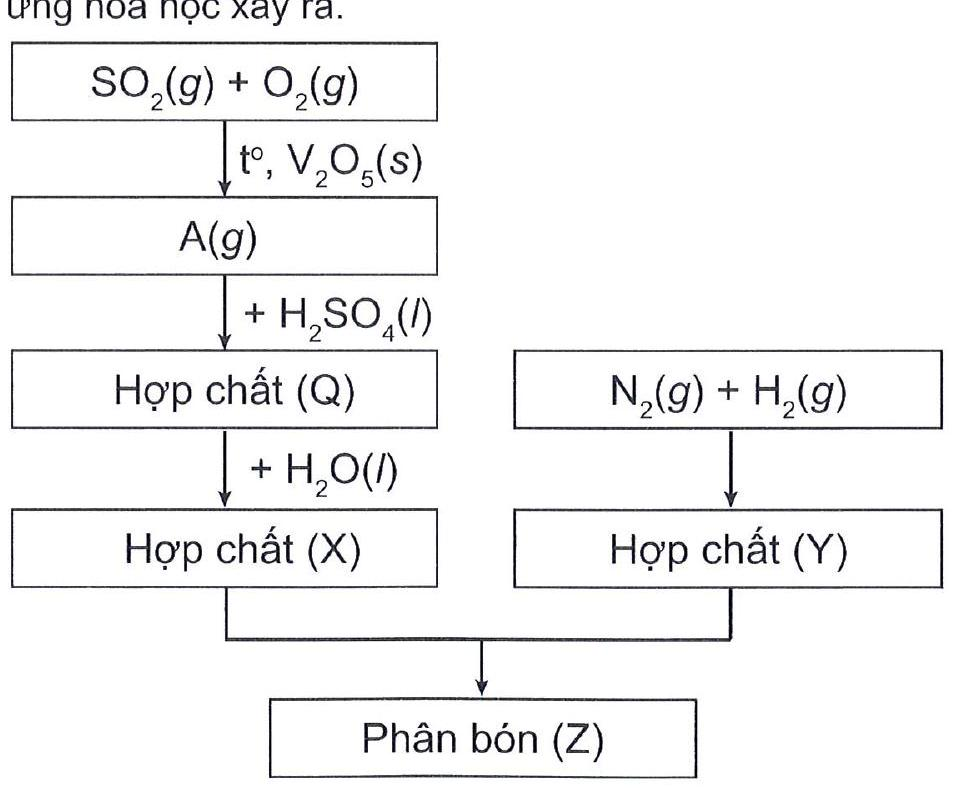
\includegraphics[max width=\textwidth, center]{2025_10_23_ae7aef68fb3b41082d29g-12}\\
7.11. Cho các dung dịch không màu của mỗi chất sau đây chứa trong các lọ mất nhãn riêng biệt: $\mathrm{Na}_{2} \mathrm{CO}_{3}, \mathrm{MgSO}_{4}, \mathrm{KNO}_{3}, \mathrm{NaOH}, \mathrm{HCl}$. Hãy trình bày cách phân biệt các dung dịch đã cho bằng phương pháp hoá học. Viết phương trình hoá học của các phản ứng xảy ra.\\
7.12*. Đặt hai cốc (A) và (B) có khối lượng bằng nhau lên hai đía cân thấy cân thăng bằng. Cho 15,9 gam $\mathrm{Na}_{2} \mathrm{CO}_{3}$ vào cốc (A) và 17,73 gam $\mathrm{CaCO}_{3}$ vào cốc (B), sau đó thêm 18 gam dung dịch $\mathrm{H}_{2} \mathrm{SO}_{4} 98 \%$ vào cốc (A) và $m$ gam dung dịch $\mathrm{HCl} 14,6 \%$ vào cốc (B) thì thấy cân thăng bằng. Tính khối lượng dung dịch HCl đã cho vào cốc (B).\\
7.13*. Đặt hai cốc (A), (B) có cùng khối lượng lên hai đĩa cân thấy cân thăng bằng. Cho vào cốc (A) 102 gam $\mathrm{AgNO}_{3}$ dạng rắn; cốc (B) 124,2 gam $\mathrm{K}_{2} \mathrm{CO}_{3}$ dạng rắn.\\
a) Thêm 100 gam dung dịch $\mathrm{HCl} 29,2 \%$ vào cốc (A); 100 gam dung dịch $\mathrm{H}_{2} \mathrm{SO}_{4} 24,5 \%$ vào cốc (B). Phải thêm bao nhiêu gam nước vào cốc (A) (hay cốc $B$ ) để cân trở lại thăng bằng?\\
b) Sau khi cân đã thăng bằng, lấy một nửa lượng dung dịch có trong cốc (A) cho vào cốc (B). Sau phản ứng, phải thêm bao nhiêu gam nước vào cốc (A) để cân trở lại thăng bằng?\\
7.14*. Bảng dưới đây cho biết độ tan của ba muối trong nước ở những nhiệt độ khác nhau ${ }^{(*)}$ :

\begin{center}
\begin{tabular}{|l|l|l|l|}
\hline
\multirow{2}{*}{Nhiệt độ của nước ( ${ }^{\circ} \mathrm{C}$ )} & \multicolumn{3}{|c|}{Độ tan (gam/100 gam nước)} \\
\hline
 & $\mathrm{Na}_{2} \mathrm{CO}_{3}$ & $\mathrm{NH}_{4} \mathrm{Cl}$ & $\mathrm{K}_{2} \mathrm{SO}_{4}$ \\
\hline
0 & 7,10 & 29,70 & 7,33 \\
\hline
20 & 21,40 & 37,56 & 11,11 \\
\hline
40 & 48,50 & 46,00 & 14,97 \\
\hline
60 & 46,50 & 55,30 & 18,20 \\
\hline
80 & 45,80 & 65,60 & 21,29 \\
\hline
100 & 45,50 & 77,30 & 24,10 \\
\hline
\end{tabular}
\end{center}

a) Vẽ đồ thị biểu diễn độ tan của ba muối theo nhiệt độ.\\
b) Độ tan của các chất rắn trong nước thường tăng theo nhiệt độ. Có nhận xét gì về độ tan của ba chất? Chất có độ tan lớn là ở nhiệt độ nào?\\
c) Chất nào có độ tan lớn nhất ở $30^{\circ} \mathrm{C}$ và $90^{\circ} \mathrm{C}$ ?

\footnotetext{${ }^{()}$Nguồn: \href{https://www.sigmaaldrich.com/VN/en/support/calculators-and-apps/solubility-ta-}{https://www.sigmaaldrich.com/VN/en/support/calculators-and-apps/solubility-ta-}\\
ble-compounds-water-temperature
}\section*{ÔN TẬP CHUONG 2}
OT2.1. Điều nào sau đây đúng về tính chất hoá học của $\mathrm{N}_{2}$ ?\\
A. $\mathrm{N}_{2}$ chỉ có tính khử.\\
B. $\mathrm{N}_{2}$ chỉ có tính oxi hoá.\\
C. $\mathrm{N}_{2}$ vừa có tính khử, vừa có tính oxi hoá.\\
D. $\mathrm{N}_{2}$ có tính acid.

OT2.2. Điều nào sau đây đúng về tính chất hoá học của $\mathrm{NH}_{3}$ ?\\
A. $\mathrm{NH}_{3}$ chỉ có tính khử.\\
B. $\mathrm{NH}_{3}$ chỉ có tính oxi hoá.\\
C. $\mathrm{NH}_{3}$ vừa có tính khử, vừa có tính oxi hoá.\\
D. $\mathrm{NH}_{3}$ có tính acid.

OT2.3. Điều nào sau đây không đúng về tính chất hoá học của dung dịch $\mathrm{HNO}_{3}$ ?\\
A. Dung dịch $\mathrm{HNO}_{3}$ có tính khử mạnh.\\
B. Dung dịch $\mathrm{HNO}_{3}$ có tính oxi hoá mạnh.\\
C. Dung dịch $\mathrm{HNO}_{3}$ đặc, nguội không phản ứng với Fe.\\
D. Dung dịch $\mathrm{HNO}_{3}$ có tính acid.

OT2.4. Phát biểu nào diễn tả đúng tính chất hoá học của $\mathrm{SO}_{2}$ ?\\
A. $\mathrm{SO}_{2}$ chỉ có tính khử.\\
B. $\mathrm{SO}_{2}$ chỉ có tính oxi hoá.\\
C. $\mathrm{SO}_{2}$ vừa có tính khử, vừa có tính oxi hoá.\\
D. $\mathrm{SO}_{2}$ không có tính khử và không có tính oxi hoá.

OT2.5. Điều nào sau đây đúng về tính chất hoá học của dung dịch $\mathrm{H}_{2} \mathrm{SO}_{4}$ đặc?\\
A. Dung dịch $\mathrm{H}_{2} \mathrm{SO}_{4}$ đặc có tính khử mạnh.\\
B. Dung dịch $\mathrm{H}_{2} \mathrm{SO}_{4}$ đặc có tính oxi hoá mạnh.\\
C. Dung dịch $\mathrm{H}_{2} \mathrm{SO}_{4}$ đặc vừa có tính khử, vừa có tính oxi hoá.\\
D. Dung dịch $\mathrm{H}_{2} \mathrm{SO}_{4}$ đặc không có tính khử, không có tính oxi hoá.

OT2.6. Hãy sắp xếp các nội dung sau cho hợp lí trong quá trình hình thành hiện tượng phú dưỡng:\\
(A) Sự phân huỷ xác động thực vật bởi vi khuẩn sử dụng nhiều oxygen trong nước gây nên tình trạng thiếu oxygen nghiêm trọng, làm chết cả hệ sinh thái.\\
(B) Ánh sáng mặt trời bị cản trở làm ảnh hưởng đến quá trình quang hợp, gây thiếu oxygen làm cho thực vật và động vật chết.\\
(C) Chất dinh dưỡng giúp thực vật và tảo sống trong nước phát triển ồ ạt.\\
(D) Phân bón và chất dinh dưỡng bị rửa trôi xuống sông, ao, hồ, ...

OT2.7. Nguyên tắc vận tải bằng đường xe lửa đối với sulfuric acid đặc chứa trong các toa thùng yêu cầu nghiêm ngặt rằng phải đóng kín ngay tức khắc vòi thoát sau khi tháo acid ra khỏi toa thùng. Hãy giải thích điều này.\\
OT2.8. Sơ đồ quy trình dưới đây mô tả các bước trong quá trình sản xuất một số loại phân bón. Hãy xác định các chất $(A),(X),(Y),(Z),(Q)$. Viết các phản ứng hoá học xảy ra.\\
Không khí $\rightarrow(\mathrm{A})$\\
Methane $\rightarrow(\mathrm{X})$\\
$(\mathrm{A})+(\mathrm{X}) \xrightarrow{\text { Haber }}(\mathrm{Y})$\\
$(\mathrm{Y}) \xrightarrow{\mathrm{H}_{2} \mathrm{SO}_{4}}$ Phân bón (Z)\\
$(\mathrm{Y}) \stackrel{\mathrm{t}^{\circ}, \mathrm{xt}}{\rightleftharpoons} \mathrm{NO} \rightarrow$ Khí nâu $\rightarrow \mathrm{HNO}_{3} \xrightarrow{+ \text { khi }(\mathrm{Y})}$ Phân bón (Q)\\
OT2.9*. Đặt hai cốc (A), (B) có khối lượng bằng nhau lên 2 đĩa cân, cân ở vị trí thăng bằng. Cho 120 gam hỗn hợp potassium hydrogencarbonate và sodium hydrogencarbonate vào cốc (A); 85 gam silver nitrate vào cốc (B). Thêm từ từ 100 gam dung dịch sulfuric acid $19,6 \%$ vào cốc (A); 100 gam dung dịch hydrochloric acid $36,5 \%$ vào cốc (B). Sau thí nghiệm, cân có ở vị trí thăng bằng không? Nếu cân không ở vị trí thăng bằng thì cần thêm bao nhiêu gam dung dịch hydrochloric acid $36,5 \%$ vào cốc nào để cân trở lại vị trí thăng bằng? Giả thiết khí $\mathrm{CO}_{2}$ không tan trong nước, bỏ qua quá trình bay hơi của nước và hydrogen chloride.

\section*{Chưong 3. ĐAI CUONE HOÁ HOC HÜU CO}
\section*{HỢP CHẤT HỮU CƠ}
VÀ HOÁ HỌC HỮU CƠ\\
8.1. Trong thành phần phân tử hợp chất hữu cơ phải luôn có nguyên tố\\
A. carbon và hydrogen.\\
B. carbon.\\
C. carbon, hydrogen và oxygen.\\
D. carbon và nitrogen.\\
8.2. Phản ứng hoá học của các hợp chất hữu cơ thường xảy ra\\
A. chậm, không hoàn toàn, không theo một hướng nhất định.\\
B. nhanh và cho một sản phẩm duy nhất.\\
C. nhanh, không hoàn toàn, không theo một hướng nhất định.\\
D. chậm, hoàn toàn, không theo một hướng nhất định.\\
8.3. Liên kết hoá học trong hợp chất hữu cơ thường là\\
A. liên kết cộng hoá trị.\\
B. liên kết kim loại.\\
C. liên kết hydrogen.\\
D. liên kết ion.\\
8.4. Các hợp chất hữu cơ thường có\\
A. nhiệt độ nóng chảy, nhiệt độ sôi cao, không tan hoặc ít tan trong nước, tan nhiều trong các dung môi hữu cơ.\\
B. nhiệt độ nóng chảy, nhiệt độ sôi thấp, tan nhiều trong nước và các dung môi hữu cơ.\\
C. nhiệt độ nóng chảy, nhiệt độ sôi thấp, không tan hoặc ít tan trong nước, tan nhiều trong các dung môi hữu cơ.\\
D. nhiệt độ nóng chảy, nhiệt độ sôi thấp, không tan trong nước.\\
8.5. Hydrocarbon là hợp chất hữu cơ có thành phần nguyên tố gồm\\
A. carbon và hydrogen.\\
B. hydrogen và oxygen.\\
C. carbon và oxygen.\\
D. carbon và nitrogen.\\
8.6. Cho các chất sau: $\mathrm{NaCl}, \mathrm{H}_{2} \mathrm{SO}_{4}, \mathrm{CH}_{4}, \mathrm{CH}_{2}=\mathrm{CH}_{2}, \mathrm{HCOONa}, \mathrm{CH}_{3}-\mathrm{CH}_{2}-\mathrm{OH}$, $\mathrm{CH}_{3}-\mathrm{CH}=\mathrm{O}, \mathrm{KOH}, \mathrm{Ba}\left(\mathrm{NO}_{3}\right)_{2}, \mathrm{CO}_{2}, \mathrm{Al}_{4} \mathrm{C}_{3}, \mathrm{KCN}$. Chất nào là chất hữu cO , chất nào là chất vô cơ?\\
8.7. Cho các chất sau: $\mathrm{CH}_{3}-\mathrm{CH}_{2}-\mathrm{CH}_{3}, \mathrm{CH}_{3}-\mathrm{NH}_{2}, \mathrm{CH}_{2}=\mathrm{CH}-\mathrm{CH}_{3}, \mathrm{CH}_{2}=\mathrm{CH}-\mathrm{COOH}$, $\mathrm{CH}_{2}=\mathrm{CH}-\mathrm{CH}=\mathrm{CH}_{2}, \mathrm{CH}_{3} \mathrm{OH}, \mathrm{CH} \equiv \mathrm{CH}, \mathrm{C}_{6} \mathrm{H}_{5} \mathrm{OH}, \mathrm{HCHO}, \mathrm{CH}_{3} \mathrm{COOCH}_{3}$, $\mathrm{H}_{2} \mathrm{~N}-\mathrm{CH}_{2}-\mathrm{COOH}$. Chất nào là hydrocarbon, chất nào là dẫn xuất của hydrocarbon?\\
8.8. Chỉ ra các nhóm chức trong các hợp chất hữu cơ sau:\\
(1) $\mathrm{CH}_{3}-\mathrm{CH}_{2}-\mathrm{OH}$;\\
(2) $\mathrm{CH}_{3}-\mathrm{O}-\mathrm{CH}_{2}-\mathrm{CH}_{3}$;\\
(3) $\mathrm{CH}_{3}-\mathrm{CH}_{2}-\mathrm{CH}_{2}-\mathrm{NH}_{2}$;\\
(4) $\mathrm{CH}_{3}-\mathrm{NH}-\mathrm{CH}_{2}-\mathrm{CH}_{3}$;\\
(5) $\mathrm{H}-\mathrm{CH}=\mathrm{O}$;\\
(6) $\mathrm{CH}_{3}-\mathrm{CH}_{2}-\mathrm{CH}_{2}-\mathrm{COOH}$.\\
8.9. Glutamic acid là một trong 20 amino acid cần thiết cho cơ thể, giữ vai trò quan trọng trong quá trình trao đổi chất của cơ thể, xây dựng cấu trúc protein và trong các biến đổi sinh hoá của hệ thần kinh trung ương. Hãy chỉ ra các nhóm chức trong glutamic acid, biết rằng glutamic acid có công thức cấu tạo như hình sau.\\
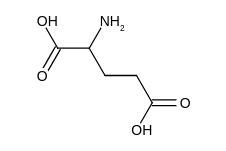
\includegraphics{smile-96a02832cbf34235a61de09d3783ad7a22b48504}\\
8.10. Phổ hồng ngoại (IR) của hợp chất hữu $\mathrm{cơ}^{\prime}(\mathrm{X})^{(*)}$ có công thức phân tử là $\mathrm{CH}_{4} \mathrm{O}$ được cho như hình bên dưới. Chất này thường được dùng trong công nghiệp để làm chất chống đông, làm dung môi trong nước rửa kính xe, chất tẩy rửa sơn, mực in máy photocopy và làm nhiên liệu cho các bếp lò loại nhỏ, ... Hãy cho biết dựa vào peak nào có thể dự đoán được $(\mathrm{X})$ là một alcohol.

\footnotetext{\begin{itemize}
  \item Nguồn: \href{https://webbook.nist.gov/cgi/cbook.cgi?Spec=C67561&Index=1&Type=IR&Large=on}{https://webbook.nist.gov/cgi/cbook.cgi?Spec=C67561\&Index=1\&Type=IR\&Large=on}
\end{itemize}
}
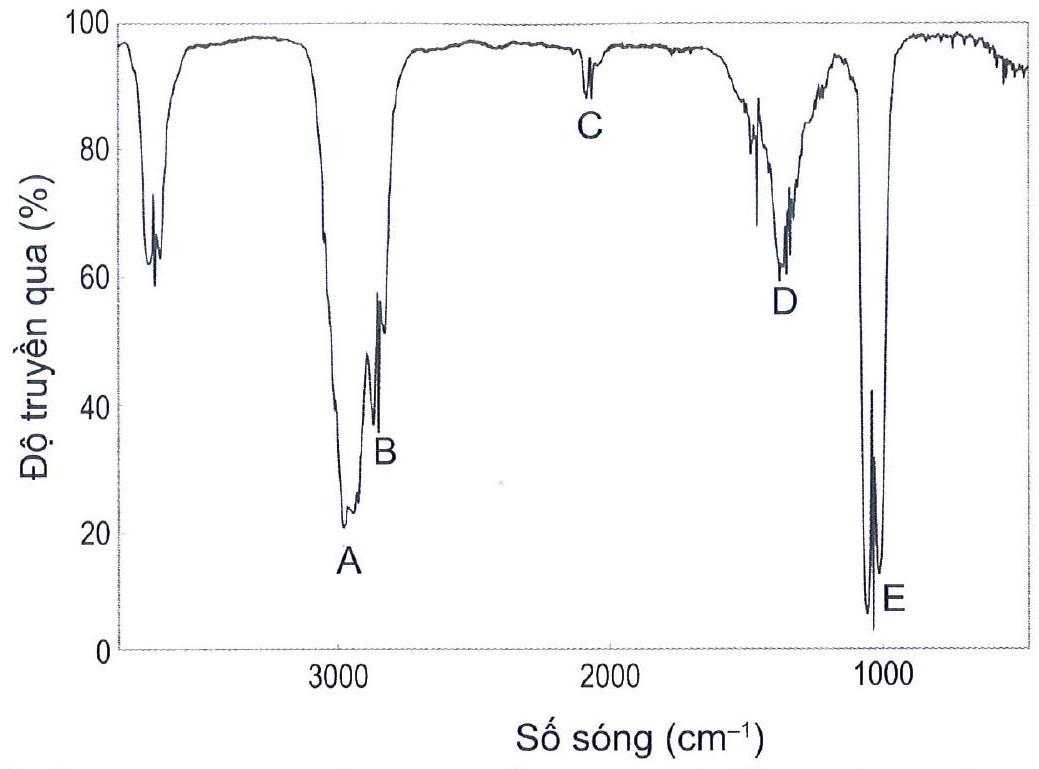
\includegraphics[max width=\textwidth, center]{2025_10_23_ae7aef68fb3b41082d29g-15(1)}\\
8.11. Phổ hồng ngoại (IR) của hợp chất hữu cơ $(Y)^{(*)}$ có công thức phân tử là $\mathrm{C}_{2} \mathrm{H}_{4} \mathrm{O}_{2}$ như hình bên dưới. Chất (Y) này được sử dụng trong nhiều ngành công nghiệp khác nhau như tạo ra polymer trong công nghiệp sản xuất sơn, chất kết dính, là dung môi hoà tan các chất hoá học, sản xuất và bảo quản thực phẩm, đặc biệt dùng để sản xuất giấm. Dựa vào phổ hồng ngoại, hãy xác định peak nào có thể chứng minh nhóm chức - COOH có trong $(\mathrm{Y})$.\\
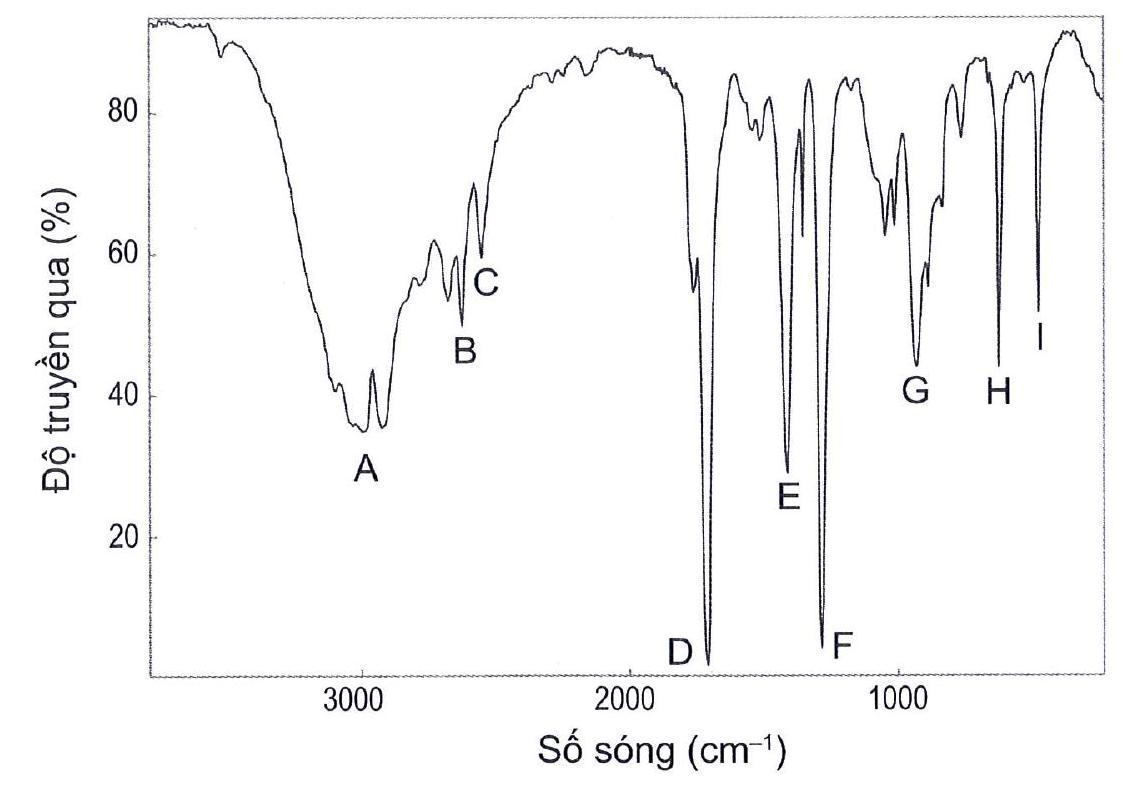
\includegraphics[max width=\textwidth, center]{2025_10_23_ae7aef68fb3b41082d29g-15}\\
8.12. Ethanol $\left(\mathrm{CH}_{3} \mathrm{CH}_{2} \mathrm{OH}\right)$ và dimethyl ether $\left(\mathrm{CH}_{3}-\mathrm{O}-\mathrm{CH}_{3}\right)$ là 2 chất có cùng công thức $\mathrm{C}_{2} \mathrm{H}_{6} \mathrm{O}$. Ethanol hiện diện trong đồ uống có cồn, nếu sử dụng

\footnotetext{${ }^{()}$Nguồn: \href{https://webbook.nist.gov/cgi/cbook.cgi?Spec=C64197&Index=2&Type=IR&Large=on}{https://webbook.nist.gov/cgi/cbook.cgi?Spec=C64197\&Index=2\&Type=IR\&Large=on}
}
nhiều sẽ gây hại cho sức khoẻ. Dimethyl ether được sử dụng làm chất đẩy trong các sản phẩm bình xịt (keo xịt tóc, keo xịt diệt côn trùng, ...). Quan sát phổ hồng ngoại ${ }^{(*)}$ sau đây và cho biết phổ này tương ứng với chất nào trong 2 chất nêu trên. Giải thích.\\
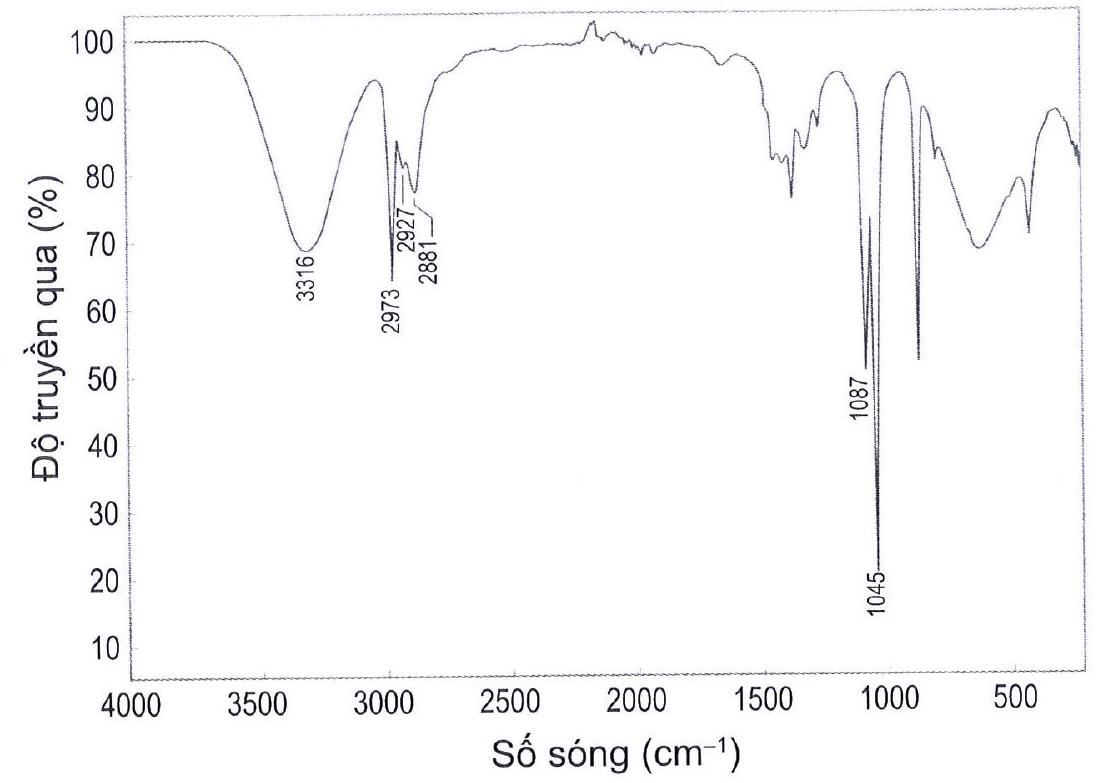
\includegraphics[max width=\textwidth, center]{2025_10_23_ae7aef68fb3b41082d29g-16(1)}\\
8.13. Heptanoic acid được ứng dụng trong mĩ phẩm, nưởc hoa và các ứng dụng tạo mùi thơm. Dựa vào phổ hồng ngoại ${ }^{(*)}$, hãy cho biết peak nào giúp dự đoán được trong hợp chất này có nhóm chức carboxyl.\\
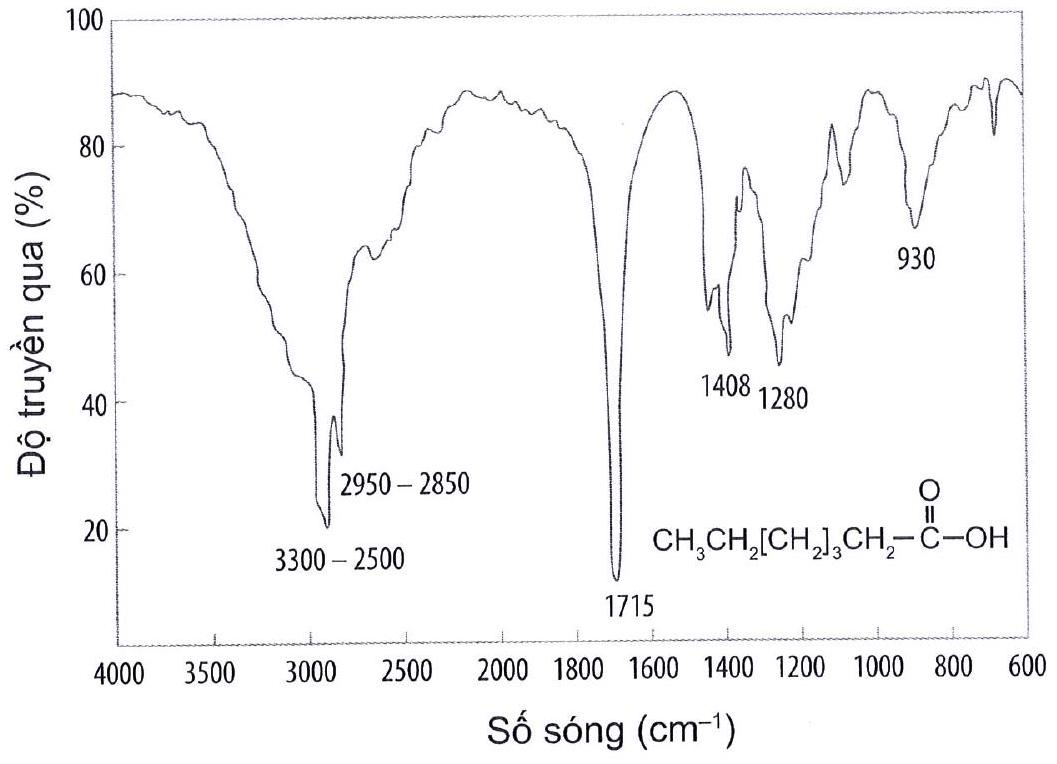
\includegraphics[max width=\textwidth, center]{2025_10_23_ae7aef68fb3b41082d29g-16(2)}

\footnotetext{${ }^{(1)}$ Nguồn: Y. R. Sharma, Elementary Organic Spectroscopy (2008), S. Chand \& Company PVT. LTD.\\
36
}
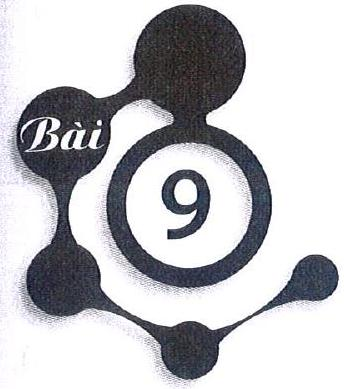
\includegraphics[max width=\textwidth, center]{2025_10_23_ae7aef68fb3b41082d29g-16}

\section*{PHƯƠNG PHÁP TÁCH VÀ TINH CHẾ HỢP CHẤT HỮU CƠ}
9.1. Phương pháp chưng cất dùng để tách các chất\\
A. có nhiệt độ sôi khác nhau.\\
B. có nhiệt độ nóng chảy khác nhau.\\
C. có độ tan khác nhau.\\
D. có khối lượng riêng khác nhau.\\
9.2. Phương pháp chiết là sự tách chất dựa vào sự khác nhau\\
A. về kích thước phân tử.\\
B. ở mức độ nặng nhẹ về khối lượng.\\
C. về khả năng bay hơi.\\
D. về khả năng tan trong các dung môi khác nhau.\\
9.3. Phương pháp kết tinh dùng để tách các chất\\
A. có nhiệt độ sôi khác nhau.\\
B. có nguyên tử khối khác nhau.\\
C. có độ tan khác nhau.\\
D. có khối lượng riêng khác nhau.\\
9.4. Phương pháp nào không dùng để tách và tinh chế các chất hữu cơ?\\
A. Phương pháp chưng cất.\\
B. Phương pháp chiết.\\
C. Phương pháp kết tinh.\\
D. Phương pháp cô cạn.\\
9.5. Nhiệt độ sôi của rượu (thành phần chính là ethanol) là $78^{\circ} \mathrm{C}$ và của nước là $100^{\circ} \mathrm{C}$. Phương pháp nào có thể tách rượu ra khỏi nước?\\
A. Cô cạn.\\
B. Lọc.\\
C. Bay hơi.\\
D. Chưng cất.\\
9.6. Phương pháp chiết được dùng để tách chất trong hỗn hợp nào sau đây?\\
A. Nước và dầu ăn.\\
B. Bột mì và nước.\\
C. Cát và nước.\\
D. Nước và rượu.\\
9.7. Cho hỗn hợp các alkane có mạch carbon thẳng sau: pentane (sôi ở $^{3} 6^{\circ} \mathrm{C}$ ), heptane (sôi ở $98^{\circ} \mathrm{C}$ ), octane (sôi ở $126^{\circ} \mathrm{C}$ ) và nonane (sôi ở $151^{\circ} \mathrm{C}$ ). Có thể tách riêng các chất đó bằng cách nào sau đây?\\
A. Chiết.\\
B. Kết tinh.\\
C. Bay hơi.\\
D. Chưng cất.\\
9.8. Để tách benzene (nhiệt độ sôi là $80^{\circ} \mathrm{C}$ ) và acetic acid (nhiệt độ sôi là $118^{\circ} \mathrm{C}$ ) ra khỏi nhau, có thể dùng phương pháp\\
A. chưng cất ở áp suất thấp.\\
B. chưng cất ở áp suất thường.\\
C. chiết bằng dung môi hexane.\\
D. chiết bằng dung môi ethanol.\\
9.9. Phương pháp kết tinh được ứng dụng trong trường hợp nào dưới đây?\\
A. Làm đường cát, đường phèn từ mía.\\
B. Giã cây chàm, cho vào nước, lọc lấy dung dịch màu để nhuộm sợi, vải.\\
C. Nấu rượu để uống.\\
D. Ngâm rượu thuốc.\\
9.10. Một hỗn hợp gồm dầu hoả có lẫn nước. Bằng cách nào để tách nước ra khỏi dầu hoả?\\
9.11. Để thực hiện tách sắc tố từ lá cây và tách các nhóm sắc tố bằng phương pháp hoá học, người ta làm như sau:

\begin{itemize}
  \item Giai đoạn 1: Sử dụng lá tươi đã loại bỏ cuống lá và gân chính. Sau đó cắt nhỏ cho vào cối sứ, nghiền nát thật nhuyễn với một ít acetone, sau đó tiếp tục thêm acetone, khuấy đều, lọc qua phễu lọc vào một bình chứa, thu được một hỗn hợp sắc tố màu xanh lục.
  \item Giai đoạn 2: Lấy một lượng benzene gấp đôi lượng dịch vừa thu được, cho vào bình, lắc đều, rồi để yên. Vài phút sau quan sát thấy dung dịch màu phân thành 2 lớp:
  \item Lớp dưới có màu vàng là màu của carotenoid hoà tan trong benzene.
  \item Lớp trên có màu xanh lục là màu của diệp lục hoà tan trong acetone. Hãy cho biết trong 2 giai đoạn của quy trình trên, người ta đã sử dụng phương pháp tách nào.\\
9.12. Hãy cho biết người ta đã sử dụng phương pháp tách nào trong các thí nghiệm sau:\\
a) Quá trình làm muối ăn từ nước biển.\\
b) Quá trình làm đường phèn từ nước mía.\\
c) Nấu rượu sau khi ủ men rượu từ tinh bột hoặc cellulose.\\
9.13. Cho quy trình thực hiện thí nghiệm sau:
\end{itemize}

Bước 1: Cân chính xác 1 gam benzoic acid thô, sau đó cho vào bình định mức dung tích 250 mL .\\
Bước 2: Cho từ từ nước sôi vào bình định mức và lắc đều cho đến khi benzoic acid tan hết.\\
Bước 3: Tiến hành lọc nóng dung dịch ở Bước 2. Sử dụng giấy lọc và phễu lọc để loại bỏ các tạp chất không tan trong benzoic acid thô.\\
Bước 4: Lọc lạnh dung dịch ở Bước 3, sau đó làm lạnh dung dịch bằng nước lạnh hoặc nước đá rồi tiến hành lọc lạnh. Tiếp theo sử dụng máy hút chân không để hút chân không thì thu được benzoic acid được giữ lại trên giấy lọc.\\
Bước 5: Cân mẫu benzoic acid trên giấy lọc vừa thu được ở Bước 4.\\
Hãy cho biết người ta đã sử dụng phương pháp tách và tinh chế nào trong thí nghiệm trên.\\
9.14. Quan sát hình mô phỏng thí nghiệm sắc kí cột sau:\\
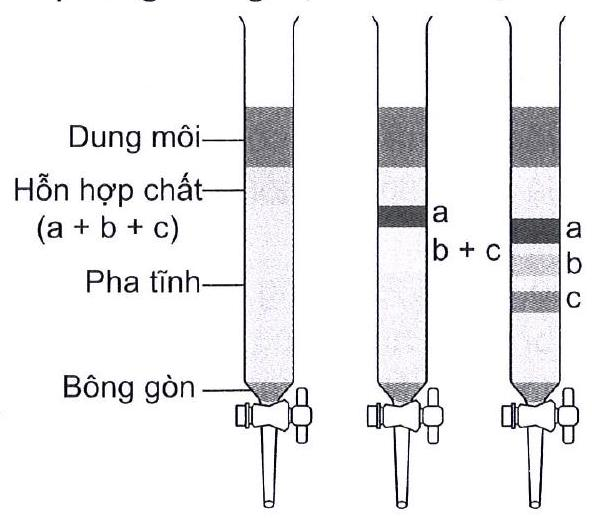
\includegraphics[max width=\textwidth, center]{2025_10_23_ae7aef68fb3b41082d29g-17}

Hãy cho biết trong điều kiện thí nghiệm:\\
a) Chất nào bị hấp phụ mạnh nhất? Chất nào bị hấp phụ kém nhất?\\
b) Chất nào hoà tan tốt hơn trong dung môi?\\
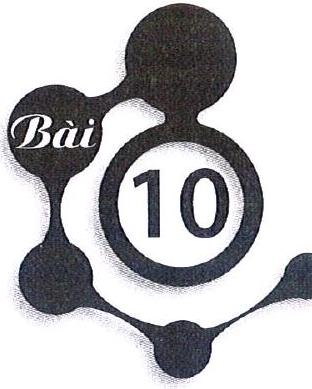
\includegraphics[max width=\textwidth, center]{2025_10_23_ae7aef68fb3b41082d29g-18}

\section*{CÔNG THỨC PHÂN TƯ HỢP CHẤT HỮU CƠ}
10.1. Acetylene là một hydrocarbon được dùng làm nhiên liệu trong đèn xì oxy-acetylene (khi tác dụng với oxygen) để hàn hay cắt kim loại. Hãy lập công thức phân tử của acetylene, biết kết quả phân tích nguyên tố của acetylene có $7,69 \% \mathrm{H}$ về khối lượng. Phân tử khối của acetylene gấp 13 lần phân tử khối của hydrogen.\\
10.2. Buta-1,3-diene là một hydrocarbon được dùng nhiều nhất trong sản xuất cao su. Hãy lập công thức phân tử của buta-1,3-diene, biết kết quả phân tích nguyên tố của buta-1,3-diene có $\frac{\% \mathrm{C}}{\% \mathrm{H}}=8$. Phân tử khối của của buta-1,3-diene gấp 1,6875 phân tử khối của oxygen.\\
10.3. Glycine là một amino acid mà cơ thể sử dụng để tạo ra protein và các chất quan trọng khác như hormone và enzyme. Hãy lập công thức phân tử của glycine, biết kết quả phân tích nguyên tố của glycine có $32,00 \% \mathrm{C} ; 6,67 \% \mathrm{H} ; 18,67 \% \mathrm{~N}$ về khối lượng, còn lại là O . Phân tử khối của glycine là 75 .\\
10.4. Phenol là hợp chất hữu cơ được sử dụng để sản xuất chất kích thích tăng trưởng ở thực vật, kích thích tố thực vật 2,4-D cũng như chất diệt cỏ dại. Hãy lập công thức phân tử của phenol, biết kết quả phân tích nguyên tố của phenol có $\mathrm{m}_{\mathrm{C}}: \mathrm{m}_{\mathrm{H}}: \mathrm{m}_{\mathrm{O}}=36: 3: 8$. Phân tử khối của phenol lớn hơn methane 78 đơn vị.\\
10.5. Thuốc nổ TNT ( $2,4,6$-trinitrotoluene) là hợp chất hữu cơ được điều chế bằng phản ứng của toluene với hỗn hợp gồm $\mathrm{HNO}_{3}$ đặc và $\mathrm{H}_{2} \mathrm{SO}_{4}$ đặc trong điều kiện đun nóng. Hãy lập công thức phân tử của TNT, biết kết quả phân tích nguyên tố của TNT có $37,00 \% \mathrm{C} ; 2,20 \% \mathrm{H} ; 42,29 \% \mathrm{O}$ về khối lượng; còn lại là N . Phân tử khối của TNT gấp khoảng 2,91 lần phân tử khối của benzene $\left(\mathrm{C}_{6} \mathrm{H}_{6}\right)$.\\
10.6. Trong ruộng lúa, ao, hồ, ... thường chứa các vật thể hữu cơ. Khi các vật thể hữu cơ đó bị phân huỷ trong điều kiện không có oxygen sinh ra hydrocarbon $(X)$ ở thể khí. Người ta đã lợi dụng hiện tượng này để làm các hầm biogas trong chăn nuôi gia súc, tạo khí ( X ) sử dụng đun nấu hoặc chạy máy, ... Hãy lập công thức phân tử của (X), biết kết quả phân tích nguyên tố của $(X)$ có $25 \% \mathrm{H}$ về khối lượng. Phân tử khối của hợp chất này được xác định thông qua kết quả phổ khối lượng ${ }^{\text {(*) }}$ với peak ion phân tử có giá trị $m / z$ lớn nhất.

\footnotetext{${ }^{()}$Nguồn: \href{https://webbook.nist.gov/cgi/cbook.cgi?ID=C74828&Mask=200}{https://webbook.nist.gov/cgi/cbook.cgi?ID=C74828\&Mask=200}
}
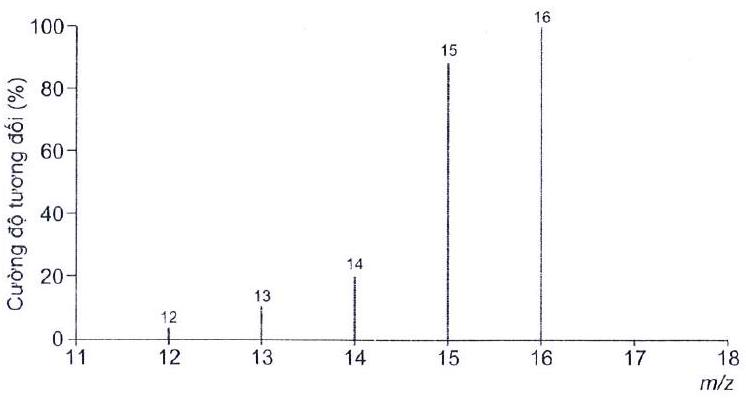
\includegraphics[max width=\textwidth, center]{2025_10_23_ae7aef68fb3b41082d29g-18(3)}\\
10.7. Hydrocarbon (Y) có tác dụng kích thích các tế bào thực vật tăng trưởng nên được sử dụng vào mục đích kích thích sự ra hoa, quả chín ở các loại cây ăn trái. Hãy lập công thức phân tử của (Y), biết kết quả phân tích nguyên tố của (Y) có $85,71 \% \mathrm{C}$ về khối lượng. Phân tử khối của hợp chất này được xác định thông qua kết quả phổ khối lượng ${ }^{(*)}$ với peak ion phân tử có giá trị $m / z$ lớn nhất.\\
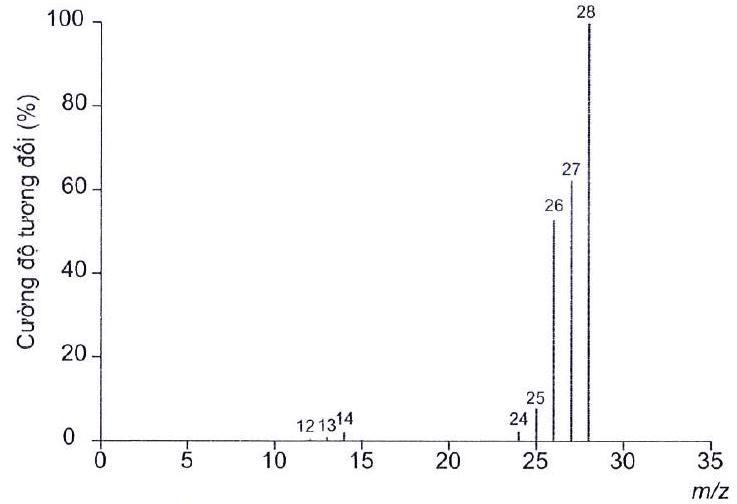
\includegraphics[max width=\textwidth, center]{2025_10_23_ae7aef68fb3b41082d29g-18(2)}\\
10.8. Diethyl ether là hợp chất dùng làm thuốc gây mê toàn thân theo đường thở. Nó cũng có tác dụng giảm đau và giãn cơ. Hãy lập công thức phân tử của diethyl ether, biết kết quả phân tích nguyên tố của hợp chất này có $64,86 \% \mathrm{C} ; 13,51 \% \mathrm{H}$ về khối lượng; còn lại là O . Khối lượng mol phân tử của diethyl ether được xác định trên phổ khối lượng ${ }^{(")}$ tương ứng với peak có giá trị $m / z$ lớn nhất.\\
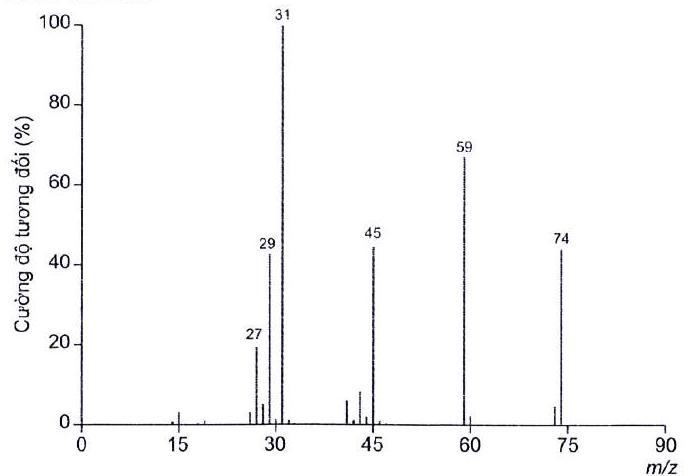
\includegraphics[max width=\textwidth, center]{2025_10_23_ae7aef68fb3b41082d29g-18(1)}

\footnotetext{(Nguồn: \href{https://webbook.nist.gov/cgi/cbook.cgi?ID=C74851&Mask=200}{https://webbook.nist.gov/cgi/cbook.cgi?ID=C74851\&Mask=200}\\
${ }^{\text {(**) }}$ Nguồn: \href{https://webbook.nist.gov/cgi/cbook.cgi?Spec=C60297&Index}{https://webbook.nist.gov/cgi/cbook.cgi?Spec=C60297\&Index} =0\&type=Mass\&Large=on
}
10.9. Formaldehyde trong dung dịch (khoảng $40 \%$ theo thể tích hoặc $37 \%$ theo khối lượng) được gọi là fomon hay formalin, được sử dụng nhiều trong y khoa với tác dụng diệt khuẩn; là dung môi giúp bảo vệ các mẫu thí nghiệm hay các cơ quan trong cơ thể con người, ... Hãy lập công thức phân tử của formaldehyde, biết kết quả phân tích nguyên tố của hợp chất này có $40 \% \mathrm{C}$ về khối lượng và $\frac{\% \mathrm{H}}{\% \mathrm{O}}=0,125$. Khối lượng mol phân tử của formaldehyde được xác định trên phổ khối lượng ${ }^{(*)}$ tương ứng với peak có giá trị $m / z$ lớn nhất.\\
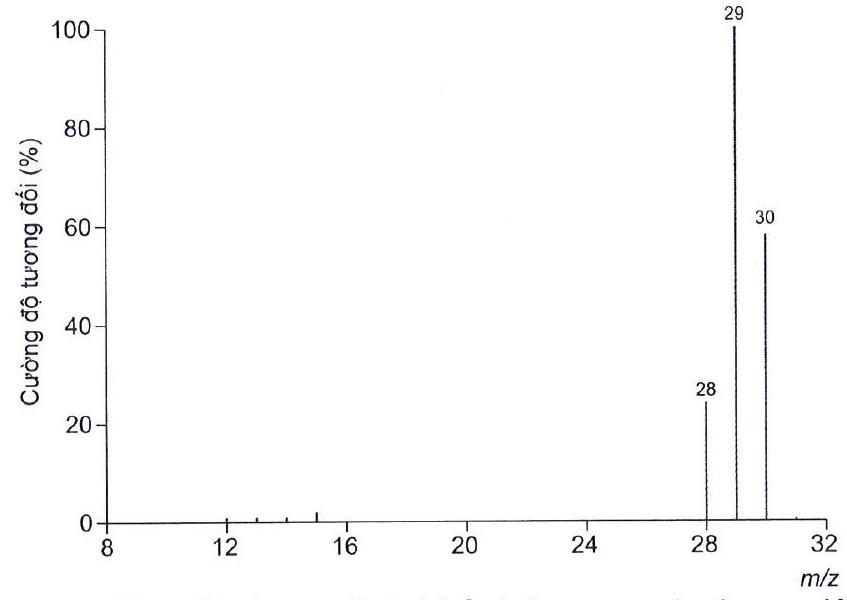
\includegraphics[max width=\textwidth, center]{2025_10_23_ae7aef68fb3b41082d29g-19}\\
10.10. Formic acid là một dung dịch khử trùng mạnh được dùng đê làm sạch trong công nghiệp hoặc trong hộ gia đình. Hãy lập công thức phân tử của formic acid, biết kết quả phân tích nguyên tố của hợp chất này có $26,09 \% \mathrm{C}$; $69,57 \% \mathrm{O}$ về khối lượng, còn lại là H . Khối lượng mol phân tử của formic acid được xác định trên phổ khối lượng ("') tương ứng với peak có cường độ tương đối xấp xỉ $60 \%$.\\
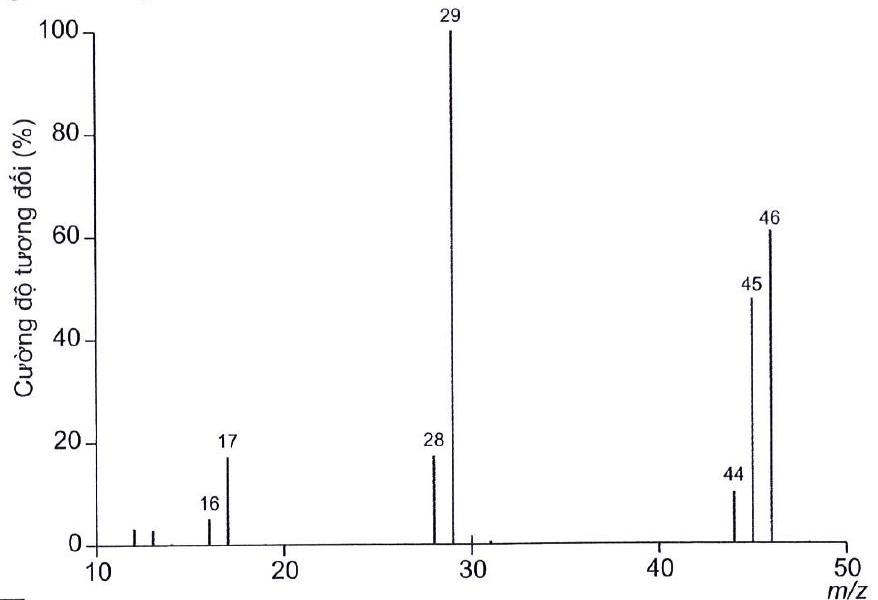
\includegraphics[max width=\textwidth, center]{2025_10_23_ae7aef68fb3b41082d29g-19(1)}

\footnotetext{${ }^{()}$Nguồn: \href{https://webbook.nist.gov/cgi/cbook.cgi?ID=C50000&Mask=200}{https://webbook.nist.gov/cgi/cbook.cgi?ID=C50000\&Mask=200}\\
(*) Nguồn: \href{https://webbook.nist.gov/cgi/cbook.cgi?ID=C64186&Mask=608}{https://webbook.nist.gov/cgi/cbook.cgi?ID=C64186\&Mask=608}
}
10.11. Hai hợp chất $(A)$ và $(B)$ đều có dạng công thức là $\left(\mathrm{CH}_{2}\right)_{n}$. Phổ MS của hai hợp chất này được cho trong hình sau:\\
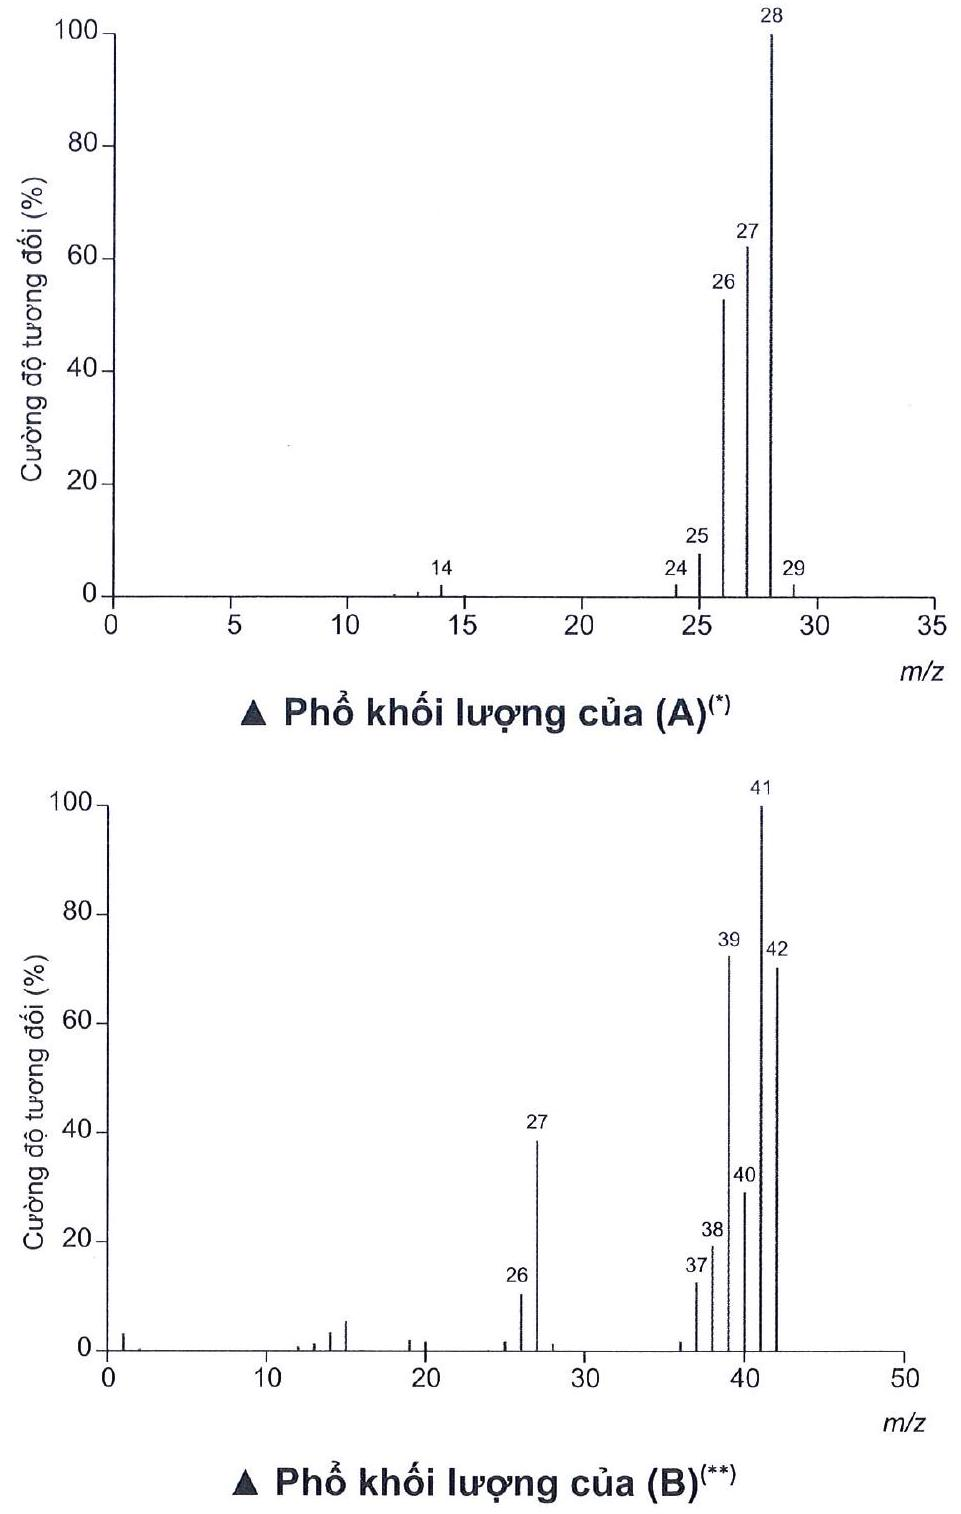
\includegraphics[max width=\textwidth, center]{2025_10_23_ae7aef68fb3b41082d29g-19(2)}

Xác định công thức phân tử của (A) và (B). Biết mảnh [ $\mathrm{M}^{+}$] của chất ( A ) có cường độ tương đối lớn nhất, mảnh [ $\mathrm{M}^{+}$] của chất ( B ) có giá trị $\mathrm{m} / \mathrm{z}$ lớn nhất.

\footnotetext{${ }^{(*)}$ Nguồn: \href{https://webbook.nist.gov/cgi/cbook.cgi?Spec=C74851&Index=0&-}{https://webbook.nist.gov/cgi/cbook.cgi?Spec=C74851\&Index=0\&-}\\
Type=Mass\&Large=on\&SVG=on\\
${ }^{\text {(**) }}$ Nguồn: \href{https://webbook.nist.gov/cgi/cbook.cgi?Spec=C115071&Index=0&Type=Mass&Large=on}{https://webbook.nist.gov/cgi/cbook.cgi?Spec=C115071\&Index=0\&Type=Mass\&Large=on}
}
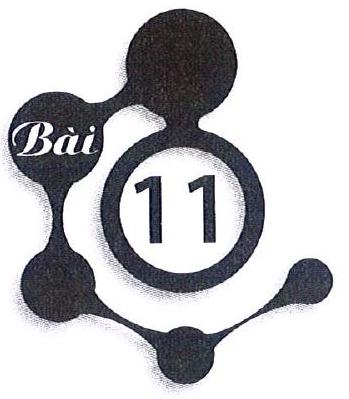
\includegraphics[max width=\textwidth, center]{2025_10_23_ae7aef68fb3b41082d29g-20(1)}

\section*{CẤU TAO HOÁ HỌC HỢP CHẤT HỮU CƠ}
11.1. Phát biểu nào sau đây là đúng?\\
A. Đồng đẳng là những chất có tỉ lệ thành phần nguyên tử trong phân tử giống nhau.\\
B. Đồng đẳng là những chất mà phân tử hơn kém nhau một hay nhiều nhóm $\mathrm{CH}_{2}$.\\
C. Đồng đẳng là những chất có cấu tạo hoá học tương tự nhau nên có tính chất hoá học cơ bản giống nhau, nhưng phân tử khác nhau một hay nhiều nhóm $\mathrm{CH}_{2}$.\\
D. Các hydrocarbon đều là đồng đẳng.\\
11.2. Phát biểu nào sau đây là đúng khi nói về đồng phân?\\
A. Những hợp chất có thành phần hoá học tương tự nhưng có cấu tạo khác nhau là những chất đồng phân.\\
B. Những hợp chất khác nhau nhưng có cấu tạo tương tự nhau là những chất đồng phân.\\
C. Những hợp chất khác nhau nhưng có cùng công thức phân tử là những chất đồng phân.\\
D. Những chất có cùng phân tử khối nhưng có cấu tạo hoá học khác nhau gọi là những chất đồng phân.\\
11.3. Cặp chất nào sau đây là đồng phân của nhau?\\
A. $\mathrm{CH}_{4}, \mathrm{CH}_{3}-\mathrm{CH}_{3}$.\\
B. $\mathrm{CH}_{3} \mathrm{OCH}_{3}, \mathrm{CH}_{3} \mathrm{CH}=\mathrm{O}$.\\
C. $\mathrm{CH}_{3} \mathrm{OH}, \mathrm{C}_{2} \mathrm{H}_{5} \mathrm{OH}$.\\
D. $\mathrm{C}_{2} \mathrm{H}_{5} \mathrm{OH}, \mathrm{CH}_{3} \mathrm{OCH}_{3}$.\\
11.4. Cặp chất nào sau đây là đồng đẳng của nhau?\\
A. $\mathrm{CH}_{3} \mathrm{OH}, \mathrm{CH}_{3} \mathrm{OCH}_{3}$.\\
B. $\mathrm{CH}_{3} \mathrm{OCH}_{3}, \mathrm{CH}_{3} \mathrm{CHO}$.\\
C. $\mathrm{HCHO}, \mathrm{CH}_{3} \mathrm{CHO}$.\\
D. $\mathrm{CH}_{3} \mathrm{CH}_{2} \mathrm{OH}, \mathrm{C}_{3} \mathrm{H}_{5}(\mathrm{OH})_{3}$.\\
11.5. Hãy cho biết dạng mạch carbon tương ứng với các chất sau:\\
(A)\\
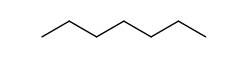
\includegraphics{smile-9e1088d2e081ba6019dab999d5decb5b66c96632}\\
(D)\\
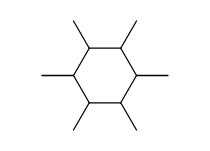
\includegraphics{smile-2251b33f9962c92f2a71e567c41b5d1b0f149d6e}\\
(B)\\
(E)\\
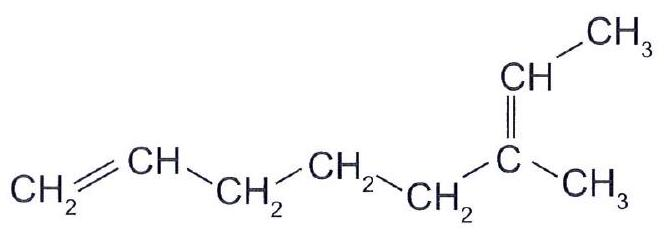
\includegraphics[max width=\textwidth, center]{2025_10_23_ae7aef68fb3b41082d29g-20}\\
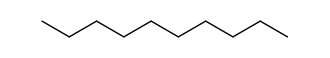
\includegraphics{smile-1046ed51bf9508ee51d1eaec3dd1ea5444b5b344}\\
(C)\\
(F)\\
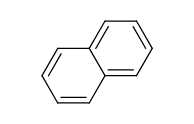
\includegraphics{smile-cb1d4acc99c1ad4fd96277dbdc55a345910d9466}\\
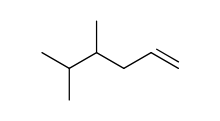
\includegraphics{smile-3a37e925033d99ff1cf5b5d6305b9ea7968330e1}\\
11.6. Viết công thức cấu tạo thu gọn của những hợp chất hữu cơ sau:\\
(A)\\
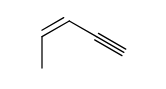
\includegraphics{smile-7f96b6606986048787ca66a5185ffbbca308d3f9}\\
(B)\\
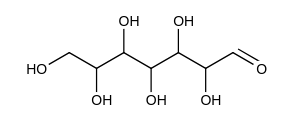
\includegraphics{smile-59bbca21a3729b30a5694f7944ccdb025e5e853e}\\
(C)\\
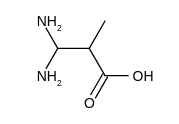
\includegraphics{smile-b032cdebc17ad81538c5a43571ee8ddbc10d20a1}\\
(D)\\
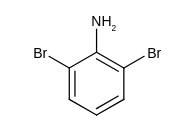
\includegraphics{smile-2f7c596b99451fc46d0efc8ace93e9a9191212ae}\\
11.7. Viết công thức cấu tạo đầy đủ của những hợp chât hữu cơ sau:\\
(A)\\
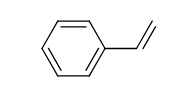
\includegraphics{smile-06ea6742efa0e8fd680b06e224b98cc666f4b2ab}\\
(B)\\
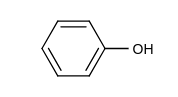
\includegraphics{smile-e30b8e6a114c4fbf4a203b224fe6a71e626c5094}\\
(C)\\
D)\\
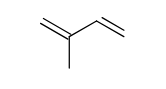
\includegraphics{smile-0495e1fdf003b1bcddcae536c89d03281513b428}\\
(E)\\
(G)\\
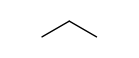
\includegraphics{smile-a342d5ae863552008934768f4012cda939808b90}\\
(H)\\
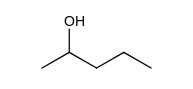
\includegraphics{smile-33f64fae2ab10c2326279a2196a8bbf200db780e}\\
(H)\\
(I)\\
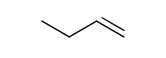
\includegraphics{smile-c7fbecaa77ab9d707e8a5cb7b3b7de216b23558b}\\
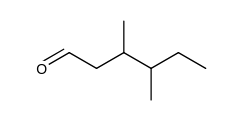
\includegraphics{smile-f3929d64c38ff73522eb28bb0f48f8a4d55ee893}\\
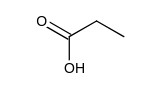
\includegraphics{smile-af15db94719476903920b3d594b83b167ada1db0}\\
11.8. Viết công thức phân tử của các hợp chất trong bài 11.6 và bài 11.7 .\\
11.9. Cho các chất sau:

\begin{center}
\begin{tabular}{ll}
$\mathrm{CH}_{3} \mathrm{CH}_{2} \mathrm{OH}(\mathrm{a})$ & $\left(\mathrm{CH}_{3}\right)_{2} \mathrm{CHCH}_{2} \mathrm{CH}_{2} \mathrm{OH}(\mathrm{e})$ \\
$\mathrm{CH}_{3} \mathrm{CH}_{2} \mathrm{CH}_{2} \mathrm{OH}(\mathrm{b})$ & $\left(\mathrm{CH}_{3}\right)_{3} \mathrm{COH}(\mathrm{g})$ \\
$\left(\mathrm{CH}_{3}\right)_{2} \mathrm{CHOH}(\mathrm{c})$ & $\mathrm{HOCH}_{2} \mathrm{CH}_{2} \mathrm{OH}(\mathrm{h})$ \\
\end{tabular}
\end{center}

$\left(\mathrm{CH}_{3}\right)_{2} \mathrm{CHCH}_{2} \mathrm{OH}(\mathrm{d})$\\
Những chất nào thuộc dãy đồng đẳng của $\mathrm{CH}_{3} \mathrm{OH}$ (methanol)?\\
11.10. Chất nào sau đây là đồng phân của $\mathrm{CH}_{3} \mathrm{COOCH}_{3}: \mathrm{CH}_{3} \mathrm{COCH}_{3}$; $\mathrm{CH}_{3} \mathrm{CH}_{2} \mathrm{COOH} ; \mathrm{CH}_{3} \mathrm{OH} ; \mathrm{C}_{2} \mathrm{H}_{5} \mathrm{OCH}_{3}$ ? Giải thích.\\
11.11. Citronellol là hợp chất được sử dụng tạo mùi hương tự nhiên có nguồn gốc từ các loại thực vật như hoa hồng, phong lữ hoặc sả, có công thức cấu tạo đầy đủ như sau:\\
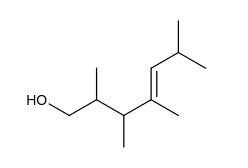
\includegraphics{smile-45749b16a338ea26579ba2f91dc788b82955ef2f}

Trên thực tế, người ta dùng dạng công thức khung phân tử để biểu diễn cấu tạo của citronellol. Hãy biểu diễn công thức đó.

\section*{ÔN TẬP CHUONG 3}
OT3.1. Để tách các chất lỏng có nhiệt độ sôi khác nhau thường dùng phương pháp\\
A. chưng cất.\\
B. chiết.\\
C. kết tinh.\\
D. sắc kí.

OT3.2. Để tách các chất từ một hỗn hợp lỏng không đồng nhất thường dùng phương pháp\\
A. chưng cất.\\
B. chiết.\\
C. kết tinh.\\
D. sắc kí.

OT3.3. Để tinh chế các chất rắn tan ra khỏi dung dịch thường dùng phương pháp\\
A. chưng cất.\\
B. chiết.\\
C. kết tinh.\\
D. sắc kí.

OT3.4. Cặp chất nào sau đây là đồng phân của nhau?\\
A. $\mathrm{CH}_{3} \mathrm{COOH}, \mathrm{HCOOCH}_{3}$.\\
B. $\mathrm{CH}_{3} \mathrm{COOH}, \mathrm{HCOOH}$.\\
C. $\mathrm{CH}_{3} \mathrm{OH}, \mathrm{C}_{2} \mathrm{H}_{5} \mathrm{OH}$.\\
D. $\mathrm{C}_{2} \mathrm{H}_{5} \mathrm{OH}, \mathrm{CH}_{3} \mathrm{OCH}_{2} \mathrm{CH}_{3}$.

OT3.5. Cặp chất nào sau đây là đồng đẳng của nhau?\\
A. $\mathrm{CH}_{4}, \mathrm{CH}_{3}-\mathrm{CH}_{2}-\mathrm{CH}_{2}-\mathrm{CH}_{3}$.\\
B. $\mathrm{CH}_{3} \mathrm{OCH}_{3}, \mathrm{CH}_{3}-\mathrm{CH}_{2} \mathrm{OH}$.\\
C. $\mathrm{HCHO}, \mathrm{CH}_{3} \mathrm{COOH}$.\\
D. $\mathrm{CH}_{2} \mathrm{OH}-\mathrm{CH}_{2} \mathrm{OH}, \mathrm{C}_{3} \mathrm{H}_{5}(\mathrm{OH})_{3}$.

OT3.6. Cho các chất sau: $\mathrm{AlCl}_{3}, \mathrm{HNO}_{3}, \mathrm{CH}_{3}-\mathrm{CH}_{2}-\mathrm{CH}_{3}, \mathrm{CH}_{2}=\mathrm{CH}-\mathrm{CH}_{2}-\mathrm{CH}_{3}$, NaOOC-COONa, $\mathrm{CH}_{2} \mathrm{OH}-\mathrm{CH}_{2} \mathrm{OH}, \mathrm{H}-\mathrm{CH}=\mathrm{O}, \mathrm{Ba}(\mathrm{OH})_{2}, \mathrm{Na}_{2} \mathrm{CO}_{3}, \mathrm{CO}$, $\mathrm{CaC}_{2}, \mathrm{NaCN}$. Chất nào là chất hữu cơ, chất nào là chất vô cơ?

OT3.7. Cho các chất sau: $\mathrm{CH}_{4}, \mathrm{CH}_{3}-\mathrm{CH}_{2}-\mathrm{NH}_{2}, \mathrm{CH}_{2}=\mathrm{CH}_{2}, \mathrm{CH}_{3}-\mathrm{COOH}$, $\mathrm{CH}_{2}=\mathrm{C}\left(\mathrm{CH}_{3}\right)-\mathrm{CH}=\mathrm{CH}_{2}, \quad \mathrm{C}_{3} \mathrm{H}_{5}(\mathrm{OH})_{3}, \quad \mathrm{CH} \equiv \mathrm{CH}, \quad \mathrm{C}_{6} \mathrm{H}_{5} \mathrm{OH}, \quad \mathrm{CH}_{3} \mathrm{CHO}$, $\mathrm{CH}_{3} \mathrm{COOCH}_{2} \mathrm{CH}_{3}, \mathrm{H}_{2} \mathrm{~N}-\mathrm{CH}\left(\mathrm{CH}_{3}\right)-\mathrm{COOH}$. Chất nào là hydrocarbon, chất nào là dẫn xuất của hydrocarbon?

OT3.8. Người ta thực hiện chiết xuất tinh dầu hồi trong phòng thí nghiệm như sau: - Giai đoạn 1 (xử lí nguyên liệu): Sau khi lấy về, quả hồi phải được xử lí sơ bộ nhằm loại bỏ các tạp chất cơ học chứa lẫn như lá, cành vụn, vỏ cây, đất cát ... (không nên loại bỏ cuống của quả hồi vì cuống quả hồi có chứa một hàm lượng tinh dầu khá cao, từ $5,49 \%-6,01 \%$ ).

\begin{itemize}
  \item Giai đoạn 2 (cán dập): Sau khi xử lí, nguyên liệu quả hồi dùng để chưng cất nên được cán dập.
  \item Giai đoạn 3: Chiết xuất tinh dầu hồi dựa trên cơ sở nhiệt độ sôi khác nhau giữa tinh dầu và nước có trong nguyên liệu.
  \item Giai đoạn 4: Tinh dầu hồi thu được ở giai đoạn 3 vẫn còn lẫn một ít nước, dù không đáng kể nhưng sẽ làm ảnh hưởng lớn đến chất lượng của tinh dầu hồi. Do đó, sau khi hoàn thành giai đoạn 3 , tinh dầu hồi phải được khử nước bằng cách để lắng yên một ngày đêm trong phễu, sau đó tiến hành tách bỏ lớp nước phía dưới. Để dễ dàng hơn cho quá trình phân lớp, có thể cho thêm một ít muối ăn để làm tăng tỉ trọng của nước còn lẫn trong tinh dầu. Sau khi tách bỏ lớp nước phía dưới, lớp tinh dầu còn lại phía trên phễu vẫn còn chứa lẫn một lượng nước rất it và sẽ được khử bỏ bằng cách xử lí với $\mathrm{Na}_{2} \mathrm{SO}_{4}$ khan.\\
Hãy cho biết phương pháp tách và tinh chế nào được sử dụng ở giai đoạn 3 và giai đoạn 4 trong quy trình trên.
\end{itemize}

OT3.9. Glycerol là hợp chất dùng làm dược phẩm để giảm cân, cải thiện hoạt động tập thể dục, giúp cơ thể bù lượng nước bị mất trong suốt thời gian bị tiêu chảy và nôn mửa cũng như làm giảm áp lực bên trong mắt ở những người bị tăng nhãn áp. Dựa vào phổ IR ${ }^{(*)}$ dưới đây, hãy cho biết peak nào có thể xác định được nhóm chức - OH có trong hợp chất $(\mathrm{X})$.\\
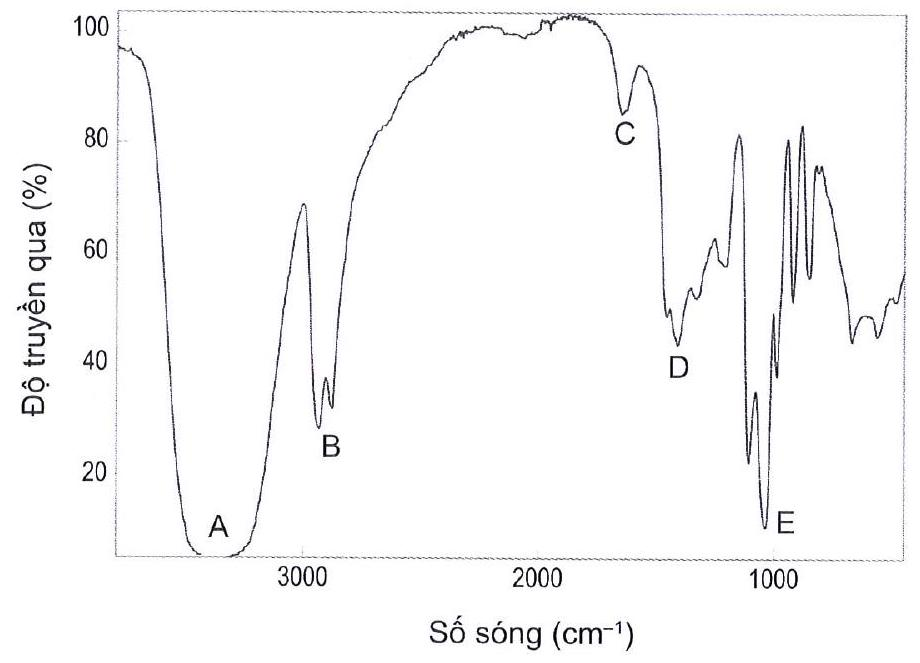
\includegraphics[max width=\textwidth, center]{2025_10_23_ae7aef68fb3b41082d29g-22}

OT3.10. Naphthalene là một hydrocarbon đóng vai trò quan trọng để tổng hợp các sản phẩm sử dụng trong sản xuất thuốc nhuộm, thuốc trừ sâu, dung môi hữu cơ và nhựa tổng hợp. Naphthalene là nguồn nguyên liệu chính cho carbaryl, sử dụng như một dạng thuốc trừ sâu nói chung. Lập công thức phân tử của naphthalene, biết kết quả phân tích nguyên tố của naphthalene có $93,75 \% \mathrm{C}$ về khối lượng. Khối lượng mol phân tử của naphthalene được xác định trên phổ khối lượng ${ }^{(* *)}$ tương ứng với peak có giá trị $m / z$ lớn nhất.

\footnotetext{() Nguồn: \href{https://webbook.nist.gov/cgi/cbook.cgi?Spec=C56815&Index=1&Type=IR&Large=on}{https://webbook.nist.gov/cgi/cbook.cgi?Spec=C56815\&Index=1\&Type=IR\&Large=on}\\
(**)Nguồn: \href{https://webbook.nist.gov/cgi/cbook.cgi?%7CD=C91203&Mask=200}{https://webbook.nist.gov/cgi/cbook.cgi?|D=C91203\&Mask=200}
}4A-BT Hóa Học 11 CTST\\
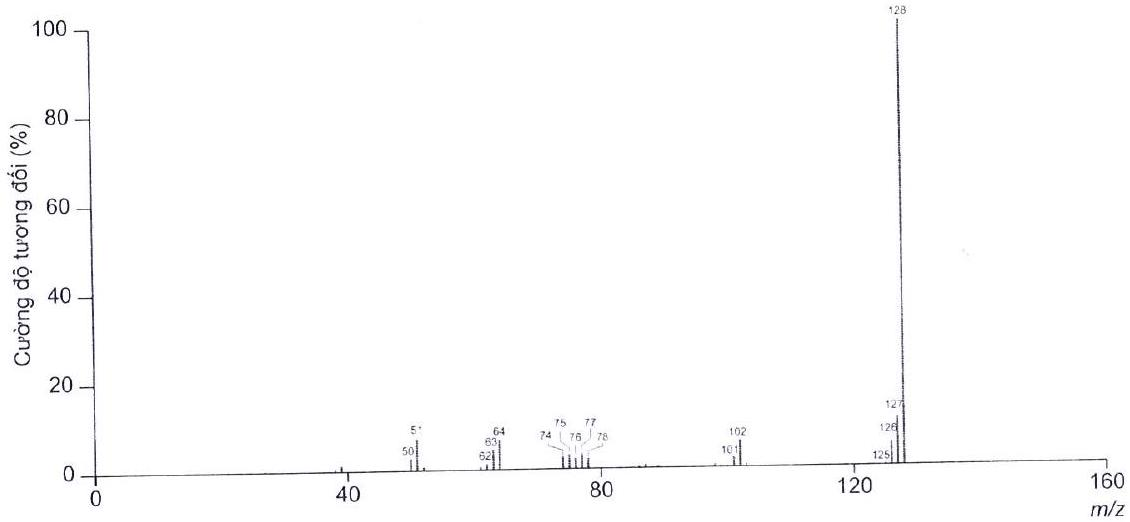
\includegraphics[max width=\textwidth, center]{2025_10_23_ae7aef68fb3b41082d29g-23(1)}

OT3.11. Acetic acid được sử dụng rộng rãi trên thế giới trong nhiều ngành công nghiệp khác nhau như tạo ra polymer ứng dụng trong sơn, chất kết dính, là dung môi hoà tan các chất hoá học, sản xuât và bảo quản thực phẩm, đặc biệt dùng để sản xuất giấm.\\
a) Lập công thức phân tử của acetic acid, biết kêt quả phân tích nguyên tố của acetic acid có $40 \% \mathrm{C}$; 53,33\% O về khối lượng; còn lại là H. Phân tử khối của acetic acid được xác định trên phổ khối lượng ${ }^{(*)}$ tương ứng với peak có giá trị $m / z$ lớn nhất.\\
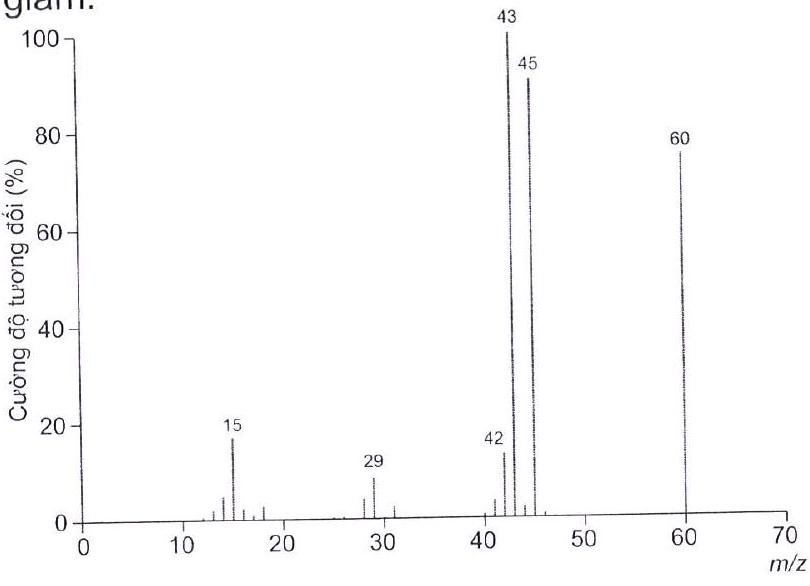
\includegraphics[max width=\textwidth, center]{2025_10_23_ae7aef68fb3b41082d29g-23}\\
b) Dựa vào phổ IR bên ${ }^{(*)}$, hãy cho biết có thể xác định được nhóm chức carboxyl có trong acetic acid từ peak nào.

\section*{Chưong 4. HYDROCARBON}
\section*{Biii}
12

\section*{ALKANE}
12.1. Theo ước tính, trung bình mỗi ngày một con bò "ợ" vào bầu khí quyển khoảng $250 \mathrm{~L}-300 \mathrm{~L}$ một chất khí có khả năng gây hiệu ứng nhà kính. Khí đó là\\
A. $\mathrm{O}_{2}$.\\
B. $\mathrm{CO}_{2}$.\\
C. $\mathrm{CH}_{4}$.\\
D. $\mathrm{NH}_{3}$.\\
12.2. Biogas là một loại khí sinh học, được sản xuất bằng cách ủ kín các chất thải hữu cơ trong chăn nuôi, sinh hoạt. Biogas được dùng để đun nấu, chạy máy phát điện sinh hoạt gia đình. Thành phần chính của biogas là\\
A. $\mathrm{N}_{2}$.\\
B. $\mathrm{CO}_{2}$.\\
C. $\mathrm{CH}_{4}$.\\
D. $\mathrm{NH}_{3}$.\\
12.3. Đồ thị dưới đây thể hiện mối tương quan giữa nhiệt độ sôi và số nguyên tử carbon trong phân tử alkane không phân nhánh được biểu diễn như sau:\\
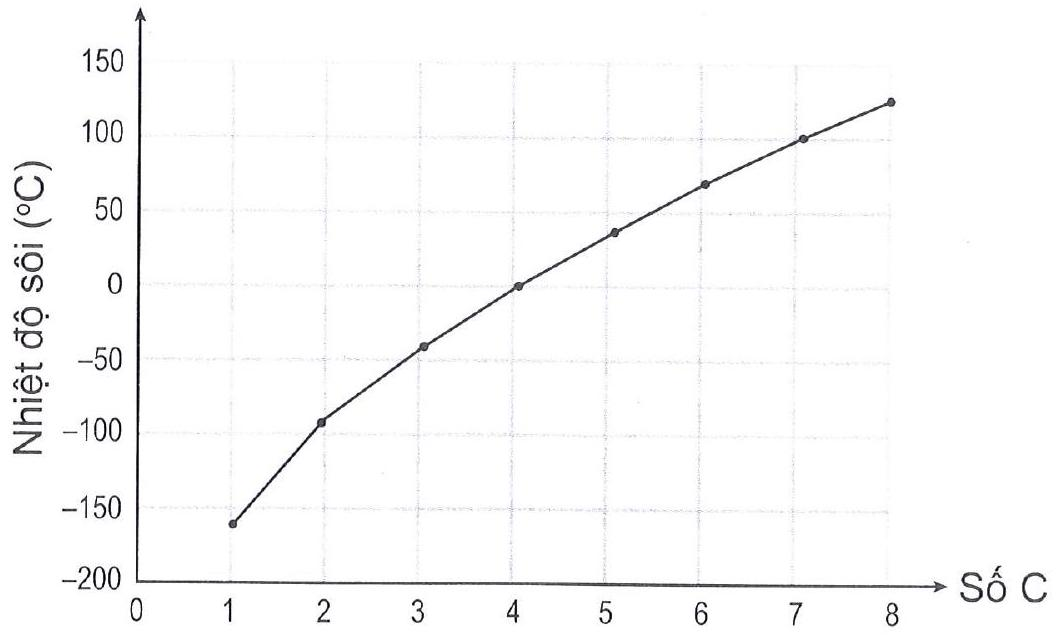
\includegraphics[max width=\textwidth, center]{2025_10_23_ae7aef68fb3b41082d29g-23(2)}

A Đồ thị biểu diễn mối tương quan giữa nhiệt độ sôi và số nguyên tử carbon trong phân tử alkane không phân nhánh

\footnotetext{${ }^{\left({ }^{*}\right)}$ Nguồn: \href{https://webbook.nist.gov/cgi/cbook.cgi?Spec=C64197&Index=0&Type=Mass&Large=on}{https://webbook.nist.gov/cgi/cbook.cgi?Spec=C64197\&Index=0\&Type=Mass\&Large=on}\\
${ }^{(* *)}$ Nguồn: \href{https://webbook.nist.gov/cgi/inchi?Spec=C64197&Index=2&Type=IR&Large=on}{https://webbook.nist.gov/cgi/inchi?Spec=C64197\&Index=2\&Type=IR\&Large=on}
}Dựa vào đồ thị đã cho, số phân tử alkane không phân nhánh ở thể khí trong điều kiện thường là\\
A. 4 .\\
B. 2.\\
C. 3 .\\
D. 1.\\
12.4. Alkane $(A)$ có công thức phân tử $C_{5} H_{12}$. $(A)$ tác dụng với chlorine khi đun nóng chỉ tạo một dẫn xuất monochloro duy nhất. Tên gọi của (A) là\\
A. pentane.\\
B. 2-methylbutane.\\
C. 2,2-dimethylpropane.\\
D. 3-methylbutane.\\
12.5. Có bao nhiêu alkane (có số nguyên tử $C \leq 5$ ) khi tác dụng với chlorine (có ánh sáng hoặc đun nóng) tạo duy nhất một sản phẩm thế monochloro?\\
A. 3 .\\
B. 2.\\
C. 1.\\
D. 4.\\
12.6. Khi cho 2,2-dimethylbutane tác dụng với chlorine thu được tối đa bao nhiêu dẫn xuất monochloro?\\
A. 3 .\\
B. 2.\\
C. 5.\\
D. 4 .\\
12.7. Cho alkane sau:\\
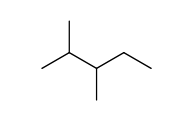
\includegraphics{smile-138fbfa4eed23b298cc0040160f1f8647e217b00}

Danh pháp thay thế của alkane trên là\\
A. 2-ethyl-3-methylbutane.\\
B. 2-methyl-3-ethylbutane.\\
C. 3,4-dimethylpentane.\\
D. 2,3-dimethylpentane.\\
12.8. Để hoàn thành bài tập gọi tên các đồng phân của alkane có công thức phân tử là $\mathrm{C}_{4} \mathrm{H}_{10}$, một bạn học sinh đã vẽ các dạng mạch carbon của alkane này, biết rằng dạng mạch carbon này chỉ chứa các liên kết đơn có thể có, sau đó bạn tiếp tục bổ sung các nguyên tử hydrogen vào dạng mạch carbon để hoàn tất bài tập. Theo em, học sinh đó đã sai ở điểm nào?\\
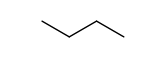
\includegraphics{smile-0a8948220f41a445f0357c545f9ef0341be3fcdd}\\
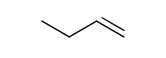
\includegraphics{smile-dfc1b3d77ce53d5ad2ffc1294e2876ef9519f309}\\
$\mathrm{C}-\mathrm{C}-\mathrm{C}-\mathrm{C}$\\
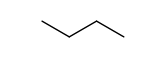
\includegraphics{smile-dba72bb4500b12f1e1ed1e009ab619c9af46acdf}\\
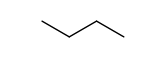
\includegraphics{smile-2dc7ecf2d61c004f09b9db4df06746bffebadd05}\\
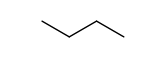
\includegraphics{smile-37652384db0dd327174a3e766e11162b936b407e}\\
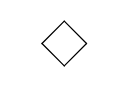
\includegraphics{smile-070e996b96a6301e7bf1bddc186ada851e092f17}\\
\includegraphics{smile-99446cb39b7095191a86025f043f4edd5a4ed665}\\
12.9. So sánh và giải thích nhiệt độ sôi của alkane mạch không phân nhánh với alkane mạch phân nhánh khi chúng có cùng số nguyên tử carbon trong phân tử.\\
12.10. Mặc dù có 5 nguyên tử carbon trong phân tử nhưng neopentane (2,2-dimethylpropane) ở thể khí trong điều kiện thường. Giải thích.\\
12.11. Em hãy cho biết xăng có tan được trong nước hay không và chất béo có tan được trong xăng hay không. Theo em, bác thợ sửa xe thường rửa tay bằng gì để sạch các vết dầu mỡ?\\
12.12. Vì sao khi tiếp xúc lâu dài với xăng sẽ làm cho da bị phồng rộp và gây đau nhức?\\
12.13. Butane là chất lỏng có thể nhìn thấy bên trong một chiếc bật lửa trong suốt, có nhiệt độ sôi thấp hơn một ít so với nhiệt độ của nước đóng băng ( $-0,5^{\circ} \mathrm{C}$ ). Tuy nhiên vì sao butane trong bật lửa lại không sôi?\\
12.14. Cho 2 -methylpropane tác dụng với chlorine (tỉ lệ mol $1: 1$, có ánh sáng) thu được tối đa bao nhiêu sản phẩm thế monochloro?\\
12.15. Khi cho 2 -methylpropane tác dụng với bromine ở $127^{\circ} \mathrm{C}$ thu được hỗn hợp 2 sản phẩm thế monobromo là 1-bromo-2-methylpropane ( $0,56 \%$ ) và 2-bromo-2-methylpropane ( $99,44 \%$ ). Xác định tỉ lệ khả năng phản ứng tương đối của nguyên tử hydrogen gắn ở nguyên tử carbon bậc I và nguyên tử carbon bậc III trong phản ứng.\\
12.16. Trong phản ứng thế của propane với chlorine ở nhiệt độ phòng khi có ánh sáng, tỉ lệ khả năng phản ứng tương đối của nguyên tử hydrogen gắn ở nguyên tử carbon bậc I và nguyên tử carbon bậc II tương ứng là $1: 4$.\\
a) Xác định tỉ lệ phần trăm các sản phẩm thế monochloro thu được trong phản ứng thế trên.\\
b) Dự đoán khả năng phản ứng và tỉ lệ phần trăm các sản phẩm thế thu được khi thay chlorine bằng bromine.\\
12.17. Giải thích tại sao các bể chứa xăng thường được quét một lớp nhũ màu trắng bạc?\\
12.18. Phân tích thành phần nguyên tố của hợp chất hữu cơ $(X)$ thu được kết quả \%C và \%H (theo khối lượng) lần lượt là $84,21 \%$ và $15,79 \%$. Phân tử khối của hợp chất ( X ) này được xác định thông qua kết quả phổ khối lượng ${ }^{(*)}$ như hình bên dưới với peak ion phân tử có giá trị $m / z$ lớn nhất.\\
\includegraphics[max width=\textwidth, center]{2025_10_23_ae7aef68fb3b41082d29g-25}\\
a) Xác định công thức phân tử của ( X ).\\
b) Nếu không có kết quả phân tích phổ khối lượng của (X), trình bày cách xác định công thức phân tử của $(X)$ dựa trên những dữ kiện em đã biết.\\
12.19*. Gọi tên alkane sau theo danh pháp thay thế:\\
a)\\
\includegraphics[max width=\textwidth, center]{2025_10_23_ae7aef68fb3b41082d29g-25(1)}

\footnotetext{${ }^{(*)}$ Nguồn: \href{https://webbook.nist.gov/cgi/cbook.cgi?ID=C111659&Mask=200}{https://webbook.nist.gov/cgi/cbook.cgi?ID=C111659\&Mask=200}
}
b)\\
\includegraphics{smile-25ae8f62ae05f2683a5c71b060be9a18f1ffe482}\\
12.20*. Chỉ số octane (octane number) là đại lượng đặc trưng cho yếu tố đo lường khả năng chống kích nổ của một nhiên liệu khi nhiên liệu này bốc cháy với không khí bên trong xi lanh của động cơ đốt trong. Nếu chỉ số octane của một mẫu xăng thấp, xăng sẽ tự cháy mà không do bu-gi bật tia lửa điện đốt. Điều này làm cho hiệu suất động cơ giảm và sẽ hư hao các chi tiết máy.

Người ta quy ước rằng chỉ số octane của 2,2,4-trimethylpentane là 100 và của heptane là 0 . Các hydrocarbon mạch vòng và mạch phân nhánh có chỉ số octane cao hơn hydrocarbon mạch không phân nhánh.

Để xác định chỉ số octane của một mẫu xăng, người ta dùng máy đo chỉ số octane.\\
a) Chỉ số octane càng cao, chất lượng xăng sẽ như thế nào?\\
b) Trong thực tế, xăng không chỉ gồm 2,2,4-trimethylpentane và heptane mà là một hỗn hợp gồm nhiều hydrocarbon khác nhau. Giả thiết một mẫu xăng chỉ gồm 8 phần thể tích 2,2,4-trimethylpentane và 2 phần thể tích heptane thì chỉ số octane của mẫu xăng này là bao nhiêu?\\
12.21*. Ethanol có thể làm tăng chỉ số octane của xăng không?\\
12.22*. Thế nào là xăng RON 92 ? RON 95 ? Xăng nào có chỉ số octane cao hơn?\\
12.23*. Tính chỉ số octane của xăng E5 và xăng E10.

\section*{HYDROCARBON KHÔNG NO}
13.1. Biểu đồ dưới đây thể hiện mối tương quan giữa nhiệt độ sôi và số nguyên tử carbon trong phân tử alkene.\\
\includegraphics[max width=\textwidth, center]{2025_10_23_ae7aef68fb3b41082d29g-26}

\section*{A Nhiệt độ sôi của một sô alkene}
Có bao nhiêu alkene trong biểu đồ ở thể khí trong điều kiện thường ( $25^{\circ} \mathrm{C}$ )?\\
A. 4.\\
B. 2.\\
C. 3.\\
D. 5.\\
13.2. Ứng với công thức phân tử $\mathrm{C}_{5} \mathrm{H}_{8}$ có bao nhiêu alkyne là đồng phân cấu tạo của nhau?\\
A. 3 .\\
B. 2.\\
C. 5.\\
D. 4 .\\
13.3. Cho các alkene sau:

\begin{enumerate}
  \item $\mathrm{CH}_{2}=\mathrm{CH}-\mathrm{CH}_{2}-\mathrm{CH}_{3}$
  \item $\left(\mathrm{CH}_{3}\right)_{2} \mathrm{C}=\mathrm{C}\left(\mathrm{CH}_{3}\right)_{2}$
  \item $\mathrm{CH}_{3}-\mathrm{CH}_{2}-\mathrm{CH}=\mathrm{CH}-\mathrm{CH}_{3}$
  \item $\mathrm{CH}_{3}-\mathrm{CH}_{2}-\mathrm{CH}=\mathrm{CH}-\mathrm{CH}_{2}-\mathrm{CH}_{3}$
\end{enumerate}

Số alkene có đồng phân hình học là\\
A. 4 .\\
B. 2.\\
C. 3 .\\
D. 1.\\
13.4. Viết công thức khung phân tử của:\\
a) propene.\\
b) pent-1-ene.\\
c) 3-methylpent-1-yne.\\
d) cis-pent-2-ene.\\
e) trans-pent-2-ene.\\
\includegraphics{smile-ac40d4a16edb3ea36ea9dcec8f6a357620ce47c4}

(A)\\
\includegraphics{smile-f089e0483638207b9da967dfa71715be0f91ac5e}

(B)\\
\includegraphics{smile-aeadeeea100e6f209653d5856dd5f15c0441d66b}

(C)\\
13.5. Cho các phân tử alkene có công thức khung phân tử dưới đây:\\
a) Gọi tên các phân tử alkene nêu trên theo danh pháp thay thế.\\
b) So sánh tương tác van der Waals giữa các phân tử alkene nêu trên.

Từ đó em có kêt luận gì?\\
13.6. Viết công thức cấu tạo và gọi tên tất cả các alkene và alkyne có công thức phân tử lần lượt là $\mathrm{C}_{5} \mathrm{H}_{10}$ và $\mathrm{C}_{5} \mathrm{H}_{8}$. Trong tất cả các chất mà em đã liệt kê, chất nào có đồng phân hình học? Viết công thức và gọi tên các đồng phân hình học đó.\\
13.7. So sánh nhiệt độ sôi của các đồng phân cis, trans của cùng một phân tử alkene. Giải thích và cho ví dụ minh hoạ.\\
13.8*. Giải thích vì sao liên kết ba $\mathrm{C} \equiv \mathrm{C}$ của một phân tử alkyne tuy giàu mật độ electron hơn so với liên kết đôi $\mathrm{C}=\mathrm{C}$ của một phân tử alkene tương ứng nhưng khả năng phản ứng cộng ( $\mathrm{X}_{2}, \mathrm{HX}, \mathrm{H}_{2} \mathrm{O}$ ) vào alkyne lại kém hơn vào alkene tương ứng?\\
13.9*. Giải thích vì sao liên kết $\pi$ của trans-but-2-ene có mật độ electron cao hơn đáng kể so với liên kết $\pi$ của trans-2,3-dibromobut-2-ene? Từ đó so sánh khả năng phản ứng cộng bromine của trans-but-2-ene và trans-2,3-dibromobut-2-ene.\\
13.10*. So sánh khả năng phản ứng cộng bromine vào liên kết ba $\mathrm{C} \equiv \mathrm{C}$ của một alkyne và vào liên kết đôi $\mathrm{C}=\mathrm{C}$ của một dibromoalkene tương ứng. Giải thích.\\
13.11. Hoàn thành các phương trình phản ứng sau (nêu rõ sản phẩm chính, phụ nếu có).\\
a) $\mathrm{CH}_{3}-\mathrm{CH}_{2}-\mathrm{CH}=\mathrm{CH}_{2}+\mathrm{Br}_{2} \longrightarrow$\\
b) $\mathrm{CH} \equiv \mathrm{C}-\mathrm{CH}_{3}+\mathrm{Br}_{2} \xrightarrow{1: 2}$\\
c) $\mathrm{CH}_{3}-\mathrm{CH}_{2}-\mathrm{CH}=\mathrm{CH}_{2}+\mathrm{HBr} \longrightarrow$\\
d) $\mathrm{CH}_{3}-\mathrm{C} \equiv \mathrm{C}-\mathrm{CH}_{3}+\mathrm{HCl} \xrightarrow[1: 1]{\mathrm{HgSO}_{4}, 60^{\circ} \mathrm{C}}$\\
e) $\mathrm{CH}_{3}-\mathrm{CH}_{2}-\mathrm{C} \equiv \mathrm{C}-\mathrm{CH}_{2}-\mathrm{CH}_{3}+\mathrm{H}_{2} \mathrm{O} \xrightarrow[60^{\circ} \mathrm{C}]{\mathrm{HgSO}_{4} / \mathrm{H}^{+}}$\\
g) $\mathrm{CH}_{2}=\mathrm{CCl}-\mathrm{CH}_{3}+\mathrm{HCl} \longrightarrow$\\
13.12. Khi cho ethylene phản ứng với nước bromine, bên cạnh sản phẩm 1,2-dibromoethane, người ta còn thu được sản phẩm 2-bromoethanol có công thức như sau:\\
\includegraphics{smile-ae878e05b4e21fadc5ffd44c28d2f91d89a751ab}

Viết phương trình phản ứng minh hoạ.\\
13.13. Khi tiến hành cho phân tử alkene cộng nước cần xúc tác là acid, sản phẩm thu được là alcohol. Nhiệt độ cần thiết cho phản ứng phụ thuộc vào bậc của alcohol tạo thành. Alcohol bậc III chỉ cần nhiệt độ dưới $25^{\circ} \mathrm{C}$, alcohol bậc II cần nhiệt độ dưới $100^{\circ} \mathrm{C}$ và alcohol bậc I cần nhiệt độ dưới $170^{\circ} \mathrm{C}$. Viết các phương trình phản ứng sau (chỉ viết sản phẩm chính):\\
a) $\mathrm{CH}_{2}=\mathrm{CH}_{2}+\mathrm{H}_{2} \mathrm{O}$ $\_\_\_\_$ $\xrightarrow{\mathrm{H}^{+}, 160^{\circ} \mathrm{C}}$\\
b) $\mathrm{CH}_{3}-\mathrm{CH}_{2}-\mathrm{CH}=\mathrm{CH}_{2}+\mathrm{H}_{2} \mathrm{O} \xrightarrow{\mathrm{H}^{+}, 90^{\circ} \mathrm{C}}$\\
c)\\
\includegraphics[max width=\textwidth, center]{2025_10_23_ae7aef68fb3b41082d29g-27}\\
13.14. Có 2 chất lỏng mất nhãn là hexane và hex-1-ene. Thuốc thử nào được dùng để phân biệt hai hoá chất này? Có thể phân biệt hai chất lỏng này dựa vào kết quả phân tích phổ hồng ngoại của chúng được không?\\
13.15. a) Đề nghị phương pháp hoá học phân biệt 2 chất lỏng mất nhãn là hex-1-yne và hex-2-yne.\\
b) Trình bày phương pháp vật lí phân biệt 2 chất lỏng mât nhãn trên.\\
13.16*. a) Vì sao nguyên tử carbon ở trạng thái lai hoá $s p$ (trong liên kết ba $\mathrm{C} \equiv \mathrm{C})$ có độ âm điện lớn hơn nguyên tử carbon ở trạng thái lai hoá $\mathrm{sp}^{2}$ (trong liên kết đôi $C=C$ ) và nguyên tử carbon ở trạng thái lai hoá $s p^{3}$ (trong liên kết đơn $\mathrm{C}-\mathrm{C}$ )? Điều này ảnh hưởng gì đến độ linh động của các nguyên tử hydrogen liên kết trực tiếp với các nguyên tử carbon ở các trạng thái lai hoá trên?\\
b) Nêu công thức cấu tạo một hydrocarbon bất kì có chứa 3 nguyên tử hydrogen linh động trong phân tử.\\
13.17. Dẫn 150 gam acetylene qua ống sắt nóng đỏ thu được 90 gam benzene. Viết phương trình phản ứng xảy ra và tính hiệu suât phản ứng.\\
13.18. Có một số loại trái cây chưa chín mà chúng ta lại muốn được sớm\\
thưởng thức chúng, chẳng hạn một quả bơ, xoài, ... Có một cách giải quyết đơn giản là cho quả bơ vào túi giấy cùng với vài quả chuối, bơ sẽ chín nhanh hơn nhiều. Giải thích cách làm trên.\\
13.19. Nhu cầu sử dụng PVC trên toàn thế giới liên tục tăng trong các năm qua. Để thu được PVC, cần đi từ monomer là vinyl chloride. Có thể điều chế vinyl chloride từ acetylene hoặc ethylene. Một trong những cách điều chế vinyl chloride từ ethylene hiện nay là theo sơ đồ:

$$
\mathrm{C}_{2} \mathrm{H}_{4} \xrightarrow{+\mathrm{Cl}_{2}}(\mathrm{X}) \xrightarrow[500^{\circ} \mathrm{C}]{-\mathrm{HCl}} \mathrm{CH}_{2}=\mathrm{CH}-\mathrm{Cl}
$$

Viết các phương trình phản ứng minh hoạ.\\
13.20. Vinyl acetate có công thức $\mathrm{CH}_{3} \mathrm{COOCH}=\mathrm{CH}_{2}$, là một ester được dùng nhiều trong lĩnh vực sản xuất keo, sơn, làm chất nhũ hoá các sản phẩm như súp, nước sốt, ... Vinyl acetate được điều chế từ hỗn hợp gồm acetic acid, ethylene và oxygen dưới sự có mặt của xúc tác palladium ở $175^{\circ} \mathrm{C} -200^{\circ} \mathrm{C}$ và áp suất 5 bar -9 bar. Viết phương trình phản ứng minh hoạ điều chế vinyl acetate.\\
13.21. Ngày nay, các nhà máy thường sử dụng chu trình khép kín hoặc tích hợp các phương pháp để nâng cao hiệu suất, hạ giá thành sản phẩm, đồng thời giảm thiểu ô nhiễm môi trường. Viết các phương trình phản ứng biểu diễn sơ đồ sản xuất sau và cho biết sơ đồ nào là tích hợp các phương pháp sản xuất vinyl chloride? Sơ đồ nào thải sản phẩm phụ ra môi trường?\\
\includegraphics[max width=\textwidth, center]{2025_10_23_ae7aef68fb3b41082d29g-27(1)}\\
\includegraphics[max width=\textwidth, center]{2025_10_23_ae7aef68fb3b41082d29g-27(2)}

\section*{ARENE (HYDROCARBON THOM)}
14.1. Công thức phân tử nào dưới đây không thể là của một arene?\\
A. $\mathrm{C}_{7} \mathrm{H}_{8}$.\\
B. $\mathrm{C}_{10} \mathrm{H}_{8}$.\\
C. $\mathrm{C}_{11} \mathrm{H}_{18}$.\\
D. $\mathrm{C}_{8} \mathrm{H}_{8}$.\\
14.2. Ứng với công thức phân tử $\mathrm{C}_{8} \mathrm{H}_{10}$ có bao nhiêu arene là đồng phân cấu tạo của nhau?\\
A. 4 .\\
B. 2.\\
C. 5.\\
D. 3 .\\
14.3. Biết độ dài liên kết $C=C$ là 134 pm , liên kết $C-C$ là 154 pm . Thực tế, 3 liên kết $\pi$ trong vòng benzene không cố định mà trải đều trên toàn bộ vòng benzene. Giá trị nào dưới đây phù hợp với độ dài liên kết giữa carbon và carbon trong phân tử benzene?\\
A. 125 pm .\\
B. 132 pm .\\
C. 160 pm .\\
D. 139 pm .

\section*{Học sinh đọc thông tin sau để trả lời các câu 14.4 và 14.5.}
Anthracene là một arene đa vòng, được điều chế từ than đá. Anthracene được dùng để sản xuất thuốc nhuộm alizarin đỏ, bảo quản gỗ, làm thuốc trừ sâu, ... Anthracene có công thức cấu tạo:\\
\includegraphics{smile-b1594e1a2f7ddfa1b903998e0cba4369cf72ada9}\\
14.4. Công thức phân tử của anthracene là\\
A. $\mathrm{C}_{16} \mathrm{H}_{18}$.\\
B. $\mathrm{C}_{14} \mathrm{H}_{8}$.\\
C. $\mathrm{C}_{14} \mathrm{H}_{12}$.\\
D. $\mathrm{C}_{14} \mathrm{H}_{10}$.\\
14.5. Số liên kết $\pi$ trong phân tử anthracene là bao nhiêu?\\
A. 9.\\
B. 7.\\
C. 8.\\
D. 6.\\
14.6. Các arene thường có chỉ số octane cao nên được pha trộn vào xăng để nâng cao khả năng chống kích nổ của xăng, như toluene và xylene thường chiếm tới $25 \%$ xăng theo thể tích. Tỉ lệ này với benzene được EPA (The U.S. Environmental Protection Agency - Cơ Quan Bảo vệ\\
môi trường Hoa Kì) quy định phải giới hạn ở mức không quá 1\% vì chúng là chất có khả năng gây ung thư.\\
Giả sử xăng có khối lượng riêng là $0,88 \mathrm{~g} / \mathrm{cm}^{3}$ thì trong 88 tấn xăng có pha trộn không quá bao nhiêu $\mathrm{m}^{3}$ benzene?\\
A. 1.\\
B. 100 .\\
C. 0,01 .\\
D. 10.\\
14.7. Gọi tên arene sau theo danh pháp thay thế\\
\includegraphics{smile-34d7af5950e933d24fc604d47a3efe58fab77190}\\
A. 1-methyl-2-ethylbenzene.\\
B. 1-ethyl-2-methylbenzene.\\
C. 2-methyl-1-ethylbenzene.\\
D. 1-ethyl-6-methylbenzene.\\
14.8. Cho hợp chất sau:\\
\includegraphics{smile-b0d7c9809d565fea7572d02acb351c41c51b0cdb}

Tên gọi của hợp chất theo danh pháp thay thế là\\
A. 4-chloro-1-bromo-3-nitrobenzene.\\
B. 4-bromo-1-chloro-2-nitrobenzene.\\
C. 4-chloro-1-bromo-5-nitrobenzene.\\
D. 4-bromo-1-chloro-6-nitrobenzene.\\
14.9. Cho hợp chất sau:\\
\includegraphics{smile-5a9182a7f6f78f56bf566d625154827f5799be6a}

Tên gọi của hợp chất theo danh pháp thay thế là\\
A. 1-bromo-3-methyl-4-nitrobenzene.\\
B. 4-bromo-2-methyl-1-nitrobenzene.\\
C. 1-methyl-2-nitro-4-bromobenzene.\\
D. 4-bromo-1-nitro-2-methylbenzene.\\
14.10*. Áp suất thể hiện bởi hơi xuất hiện trên bề mặt chất lỏng (hoặc rắn) được gọi là áp suất hơi. Một chất lỏng (hoặc rắn) có áp suất hơi cao ở nhiệt độ bình thường được gọi là chất dễ bay hơi. Khi nhiệt độ của chất lỏng (hoặc rắn) tăng, động năng của các phân tử cũng tăng lên làm cho số phân tử chuyển thành thể hơi tăng theo, do đó áp suất hơi tăng.\\
Đồ thị dưới đây biểu diễn áp suất hơi của 3 chất lỏng khác nhau là benzene $\left(\mathrm{C}_{6} \mathrm{H}_{6}\right)$, tetrahydrofuran $\left(\mathrm{C}_{4} \mathrm{H}_{8} \mathrm{O}\right)$ và acetone $\left(\mathrm{C}_{3} \mathrm{H}_{6} \mathrm{O}\right)$ theo nhiệt độ.\\
\includegraphics[max width=\textwidth, center]{2025_10_23_ae7aef68fb3b41082d29g-29(1)}

Sử dụng đồ thị trên để trả lời các câu hỏi sau đây:\\
a) Trong cùng một nhiệt độ, chất nào dễ bay hơi nhất trong số 3 chất lỏng nêu trên?\\
b) Chỉ dựa vào đồ thị, ở điều kiện áp suất bình thường ( 1 atm hay 760 torr, khoảng 1,013 bar), mỗi chất lỏng trên có nhiệt độ sôi là bao nhiêu?\\
c) Nếu đặt một cốc chứa benzene lỏng vào trong một bình kín chứa hơi benzene ở $73^{\circ} \mathrm{C}$ và 600 torr (khoảng 0,799 bar). Sau 10 phút, thể tích chất lỏng trong cốc có thay đổi không? Giải thích.\\
14.11. Viết công thức cấu tạo và gọi tên các arene có công thức phân tử $\mathrm{C}_{9} \mathrm{H}_{12}$.\\
14.12. AQI (Air Quality Index - chỉ số chất lượng không khí) được xem là thước đo mức độ ô nhiễm không khí. Khi chỉ số AQI càng lớn thì những rủi ro đối với sức khoẻ cộng đồng càng cao. Chỉ số AQI tập trung vào các vấn đề về sức khoẻ có thể gặp trong vòng vài giờ hoặc vài ngày sau khi hít thở không khí ô nhiễm.\\
EPA tính toán chỉ số AQI với 5 thông số ô nhiễm không khí chủ yếu gồm ozone mặt đất; ô nhiễm phân tử (đánh giá quá chỉ số bụi mịn PM 2.5 và PM 10); carbon monoxide (CO); sulfur dioxide (SO2) và nitrogen dioxide ( $\mathrm{NO}_{2}$ ).

Đối với mỗi chất gây ô nhiễm, EPA đã thiết lập các tiêu chuẩn chất lượng không khí, trong đó, từng khoảng giá trị AQI được quy định để phản ánh mức độ ô nhiễm không khí. Ví dụ đối với carbon monoxide, EPA đưa ra thang cảnh báo sau:

\begin{figure}[h]
\begin{center}
  \includegraphics[width=\textwidth]{2025_10_23_ae7aef68fb3b41082d29g-29}
\captionsetup{labelformat=empty}
\caption{$\triangle A Q 1$ (theo carbon monoxide)}
\end{center}
\end{figure}

Khí carbon monoxide được thải ra từ hầu hết các nguồn phát thải của các phương tiện giao thông đường bộ, đường thuỷ, đường hàng không, nhà máy công nghiệp, cháy rừng, ... Theo em, carbon monoxide đạt mức cao nhất trong những ngày thời tiết lạnh hay nắng nóng? Vì sao?

Học sinh đọc thông tin sau để trả lời các câu 14.13 và 14.14.\\
Cumene (isopropylbenzene) là một arene ở thể lỏng trong điều kiện thường, có mùi dễ chịu. Cumene được sản xuất từ quá trình chưng cất nhựa than đá và các phân đoạn dầu mỏ hoặc bằng cách alkyl hoá benzene với propene, xúc tác là acid.\\
Khoảng $95 \%$ cumene được sử dụng làm chất trung gian trong sản xuất phenol và acetone. Các ứng dụng khác như trong sản xuất styrene, $\alpha$-methylstyrene, acetophenone, chất tẩy rửa; làm chât pha loãng cho sơn; làm dung môi cho chất béo và nhựa; in ấn và sản xuất cao su. Một lượng nhỏ được sử dụng trong pha chế xăng và là thành phần của nhiên liệu hàng không có chỉ số octane cao.\\
Đã có bằng chứng rõ rệt về khả năng gây ung thư của cumene đối với chuột. Ơ' người, cumene thuộc nhóm có thể gây ung thư. Cumene được thải ra từ quá trình đốt cháy không hoàn toàn nhiên liệu hoá thạch từ các phương tiện giao thông, dầu tràn, vận chuyển và phân phối nhiên liệu hoá thạch hoặc bốc hơi từ các trạm xăng. Ngoài ra, các nguồn thải khác từ việc sử dụng cumene làm dung môi, từ các nhà máy dệt và kể cả từ khói thuốc lá, ... cũng là một trong những nguyên nhân gây nên bệnh ung thư ở người.\\
Bảng sau đây thống kê một số nguồn sản sinh cumene trong đời sống, sinh hoạt, sản xuất.

\begin{center}
\begin{tabular}{|c|c|l|}
\hline
Nguồn & Tỉ lệ phát thải & \multicolumn{1}{|c|}{Ghi chú} \\
\hline
\multirow{2}{*}{Sản xuất} & $0,08 \mathrm{~kg} /$ tấn cumene & Được kiểm soát \\
\cline { 2 - 3 }
 & $0,27 \mathrm{~kg} /$ tân cumene & Không được kiểm soát \\
\hline
\end{tabular}
\end{center}

\begin{center}
\begin{tabular}{|l|l|l|}
\hline
\multicolumn{1}{|c|}{Nguồn} & \multicolumn{1}{c|}{Tỉ lệ phát thải} & \multicolumn{1}{c|}{Ghi chú} \\
\hline
\begin{tabular}{l}
Xe chạy \\
động cơ xăng \\
\end{tabular} & $0,0002-0,0009 \mathrm{~g} / \mathrm{km}$ & Có bộ chuyển đổi xúc tác \\
\hline
Máy photocopy & $0,002 \mathrm{~g} / \mathrm{km}$ & Không có bộ chuyền đồi xúc tác \\
\hline
\end{tabular}
\end{center}

14.13. Bộ chuyển đổi xúc tác trong động cơ xăng có khả năng giảm thiểu tối đa bao nhiêu phần trăm cumene so với trường hợp không có bộ chuyển đổi xúc tác?\\
14.14. a) Tính khối lượng cumene tối đa phát thải từ 1000000 xe ô tô chạy động cơ xăng (có bộ chuyển đổi xúc tác) trong 1 năm. Giả sử bình quân một tháng, mỗi xe ô tô chạy 3000 km .\\
b) Một cửa hàng có 10 máy photocopy. Bình quân mỗi máy sử dụng liên tục 12 giờ/ngày. Trong một tháng (30 ngày), khối lượng cumene tối đa phát thải từ 1000 cửa hàng có quy mô trên là bao nhiêu?\\
14.15. Dùng công thức cấu tạo, hãy viết phương trình hoá học ở các phản ứng sau:\\
a) styrene $+\mathrm{Br}_{2}\left(\right.$ trong $\left.\mathrm{CCl}_{4}\right) \longrightarrow$\\
b) ethylbenzene $+\mathrm{Cl}_{2} \xrightarrow{\mathrm{Fe}}$\\
c) ethylbenzene $+\mathrm{HNO}_{3}($ đặc $) \xrightarrow{\mathrm{H}_{2} \mathrm{SO}_{4}(\text { dặc }), 60^{\circ} \mathrm{C}}$\\
d) cumene $+\mathrm{H}_{2} \xrightarrow{\mathrm{Ni}, \mathrm{t}^{\circ}}$\\
e) ethylbenzene $+\mathrm{KMnO}_{4}+\mathrm{H}_{2} \mathrm{SO}_{4} \xrightarrow{80^{\circ} \mathrm{C}}$\\
g) tert-butylbenzene $+\mathrm{KMnO}_{4}+\mathrm{H}_{2} \mathrm{SO}_{4} \xrightarrow{80^{\circ} \mathrm{C}}$\\
14.16. Với sự hiện diện của bột nhôm, có bao nhiêu sản phẩm monobromo dự kiến thu được do quá trình bromine hoá $p$-xylene, o-xylene và $m$-xylene. Viết các phương trình phản ứng minh hoạ.\\
14.17. $(\mathrm{H})$ là hydrocarbon có công thức phân tử là $\mathrm{C}_{9} \mathrm{H}_{12} .(\mathrm{H})$ không làm mất màu nước bromine nhưng $(\mathrm{H})$ làm mất màu dung dịch thuốc tím đã được acid hoá (ví dụ dung dịch $\mathrm{KMnO}_{4}$ trong $\mathrm{H}_{2} \mathrm{SO}_{4}$ ), thu được sản phẩm là terephthalic acid. Xác định công thức cấu tạo của $(\mathrm{H})$ và viết phương trình phản ứng xảy ra. Cho biết công thức cấu tạo của terephthalic acid là:\\
\includegraphics{smile-c61b6bfc2ee8509c73527a65d04f20529e06f3b2}\\
\includegraphics{smile-ddf79f13631d80950f2152839f64ab3ba881c9e5}

benzene\\
\includegraphics{smile-e485dd6ad92b1d0733061844c9a75a820b823c1c}

55\\
toluene\\
\includegraphics{smile-c8932c6fbbbab5a6ed66d67dfbaa6a83f5e17f09}

75\\
tert-butylbenzene\\
\includegraphics{smile-e2401695b6a5fa730a2f22cc2836c9ac2d84e254}

0,14\\
chlorobenzene\\
\includegraphics{smile-688c8a55d789adc73821459f4df92db325df1969}

0,001\\
methyl benzoate

Học sinh đọc thông tin sau để trả lời các câu 14.18 và 14.19.\\
Trong phản ứng nitro hoá benzene và các hợp chất có vòng benzene, nếu quy ước tốc độ phản ứng tại một trong các carbon bất kì của benzene là 1,0 thì tỉ lệ tốc độ phản ứng tương đối của các vị trí trong vòng benzene ở một số hợp chất được cho như sau:\\
14.18. Từ dữ liệu tỉ lệ tốc độ phản ứng tương đối của các vị trí trong vòng benzene của một số hợp chất đã cho trên, hãy cho biết:\\
a) Nhóm thế nào làm tăng hoạt( ${ }^{(*)}$ và giảm hoạt ${ }^{(*)}$ trong vòng benzene ở trên.\\
b) Nitro hoá toluene thu được hỗn hợp 3 sản phẩm là $o$-nitrotoluene, $m$-nitrotoluene và $p$-nitrotoluene với tỉ lệ phần trăm mỗi sản phẩm là bao nhiêu?\\
c) Câu hỏi tương tự khi nitro hoá tert-butylbenzene thu được hỗn hợp 3 sản phẩm ở các vị trí ortho, meta và para?\\
d) Vì sao sản phẩm thế ở vị trí ortho trong phản ứng nitro hoá tert-butylbenzene\\
lại giảm hẳn so với trong phản ứng nitro hoá toluene?\\
e) Nhận xét tỉ lệ phần trăm sản phẩm thế meta trong các phản ứng nitro hoá toluene và tert-butylbenzene. Rút ra kết luận.\\
14.19. Cũng từ dữ liệu đã cho trên, hãy cho biết:\\
a) Phần trăm sản phẩm thế ở các vị trí ortho, meta, para khi nitro hoá chlorobenzene và methyl benzoate.\\
b) So sánh khả năng nitro hoá của chlorobenzene và methyl benzoate với khả năng nitro hoá của toluene và tert-butylbenzene. Rút ta kết luận.\\
c) Phát biểu quy luật thế vào vòng benzene.\\
14.20. Benzene là một hoá chất công nghiệp được sử dụng rất rộng rãi. Benzene được sử dụng để sản xuất chất dẻo, nhựa, sợi tổng hợp, chất bôi trơn cao su, thuốc nhuộm, chất tẩy rửa, dược phẩm và thuốc trừ sâu, ...\\
Benzene có thể được tìm thấy trong keo dán, chất kết dính, sản phẩm tẩy rửa, dụng cụ tẩy sơn, khói thuốc lá và xăng. Trong tự nhiên, khi các\\
(')Nhóm thế làm tăng hoạt vòng benzene là các nhóm thế làm tăng mật độ electron trong vòng, làm cho phản ứng thế (halogen hoá, nitro hoá, ...) xảy ra dễ hơn so với benzene và hướng thế ưu tiên vào các vị trí ortho hoặc para so với nhóm thê đó.\\
(") Nhóm thế làm giảm hoạt vòng benzene là các nhóm thể làm giảm mật độ electron trong vòng, làm cho phản ứng thế (halogen hoá, nitro hoá, ...) xảy ra khó hơn so với benzene và hướng thế ưu tiên vào vị trí meta so với nhóm thế đó.\\
ngọn núi lửa hoạt động hay cháy rừng, người ta phát hiện ra sự có mặt của benzene. Ngoài ra, benzene còn được tìm thấy trong dầu thô và là thành phần không thể thiếu của xăng. Vì benzene dễ bay hơi nhanh khỏi nước hoặc đất nên việc benzene rò rỉ từ các bể chứa hoặc bãi chôn lấp sẽ làm ô nhiễm các giếng nước sinh hoạt lân cận.\\
Cách tiếp xúc phổ biến nhất với benzene là khi chúng ta đổ xăng. Ngoài ra, khi sử dụng các sản phẩm có chứa benzene nêu trên hoặc khi tiếp xúc với nguồn nước ô nhiểm có chứa benzene, chúng ta đã vô tình đưa benzene vào cơ thể.\\
Em hãy đề nghị cách để giảm thiểu sự tiếp xúc với benzene trong đời sống.\\
14.21. Toluene có giá trị thương mại thấp hơn nhiều so với benzene. Chính vì lí do đó nên người ta đã tiến hành loại bỏ nhóm methyl khỏi toluene bằng một quá trình gọi là dealkyl hoá. Toluene được trộn với hydrogen ở nhiệt độ từ $550^{\circ} \mathrm{C}$ đến $650^{\circ} \mathrm{C}$ và áp suất từ 30 atm đến 50 atm , với hỗn hợp gồm silicon dioxide ( $\mathrm{SiO}_{2}$ ) và aluminium oxide ( $\mathrm{Al}_{2} \mathrm{O}_{3}$ ) làm xúc tác.\\
Viết phương trình phản ứng dealkyl hoá toluene thành benzene.\\
14.22*. Với cách viết công thức cấu tạo gồm 3 liên kết đôi xen lẫn 3 liên kết đơn trong vòng 6 cạnh, có thể gọi tên benzene là cyclohexe-1,3,5-triene được không? Vì sao?\\
14.23*. Khi cho ethylbenzene phản ứng với bromine khan, xúc tác $\mathrm{FeBr}_{3}$ thu được hỗn hợp 3 sản phẩm thế theo sơ đồ sau:\\
\includegraphics[max width=\textwidth, center]{2025_10_23_ae7aef68fb3b41082d29g-31}

Giải thích tỉ lệ \% các sản phẩm hình thành.

\section*{ÔN TẬP CHUONG 4}
OT4.1. Alkane (A) có công thức phân tử $\mathrm{C}_{8} \mathrm{H}_{18}$. (A) tác dụng với chlorine đun nóng chỉ tạo một dẫn xuất monochloro duy nhất. Tên gọi của (A) là\\
A. octane.\\
B. 2-methylheptane.\\
C. 2,2-dimethylhexane.\\
D. 2,2,3,3-tetramethylbutane.

OT4.2. Cho các alkene sau: $\mathrm{CH}_{2}=\mathrm{CH}-\mathrm{CH}_{3} ;\left(\mathrm{CH}_{3}\right)_{2} \mathrm{C}=\mathrm{C}\left(\mathrm{CH}_{3}\right)_{2} ; \mathrm{CH}_{3} \mathrm{CH}=\mathrm{CHCH}_{3}$ và $\mathrm{CH}_{3} \mathrm{CH}=\mathrm{CHC}_{2} \mathrm{H}_{5}$. Số alkene có đồng phân hình học là\\
A. 2.\\
B. 4.\\
C. 1.\\
D. 3 .

OT4.3. Arene (B) có công thức phân tử $\mathrm{C}_{8} \mathrm{H}_{8}$. Khi có mặt bột sắt, (B) tác dụng với bromine tạo một sản phẩm thế monobromo duy nhất. Số công thức cấu tạo phù hợp với (B) là\\
A. 3 .\\
B. 4.\\
C. 1.\\
D. 2 .

OT4.4. Hoá lỏng một alkane ở thể khí là cách để tối ưu hoá khả năng lưu trữ alkane trong các thiết bị. Để hoá lỏng một alkane ở thể khí, người ta có thể tiến hành trong điều kiện nhiệt độ thấp hơn nhiệt độ sôi của alkane. Ví dụ chúng ta có thể hoá lỏng propane ở nhiệt độ thấp hơn $-42^{\circ} \mathrm{C}$ hay methane xuống thấp hơn nhiệt độ $-162^{\circ} \mathrm{C}$.

Tuy nhiên cách làm này rất tốn kém, không đạt hiệu quả kinh tế nên ît được áp dụng, mà thay vào đó người ta hoá lỏng alkane bằng cách nén chúng dưới áp suất cao. Để propane là chất lỏng ở nhiệt độ phòng, propane phải được giữ trong bình ở áp suất khoảng 850 kPa , tức khoảng $8,5 \mathrm{~atm}$. Với methane phải khoảng 32000 kPa , tức khoảng 320 atm và butane khoảng 230 kPa , tức khoảng $2,3 \mathrm{~atm}$.\\
a) Alkane nào trong số 3 alkane đã nêu dễ hoá lỏng hơn?\\
b) Khí hoá lỏng nào trong số 3 khí hoá lỏng trên cần phải lưu trữ trong thiết bị thép cực bền? Vì sao?

OT4.5. Ở các nước Mỹ, Úc và một số quốc gia khác, khí hoá lỏng (LPG - Liquefied Petroleum Gas) được sử dụng nhiều làm nhiên liệu là propane hoá lỏng. Em hãy tính xem một bình khí hoá lỏng chứa 12 kg propane có thể cung cấp bao nhiêu lít khí propane ở $25^{\circ} \mathrm{C}, 1$ bar.

OT4.6. Quan sát biểu đồ thể hiện nhiệt độ sôi của 6 alkane đầu tiên.

\begin{figure}[h]
\begin{center}
\captionsetup{labelformat=empty}
\caption{Nhiệt độ (K)}
  \includegraphics[width=\textwidth]{2025_10_23_ae7aef68fb3b41082d29g-32}
\end{center}
\end{figure}

$\Delta$ Biểu đồ thể hiện nhiệt độ sôi của các alkane từ $\mathrm{CH}_{4}$ đến $\mathrm{C}_{6} \mathrm{H}_{14}$\\
a) Có bao nhiêu alkane ở thể khí trong điều kiện thường?\\
b) Giải thích tại sao neopentane cũng ở thể khí trong điều kiện thường.\\
c) Cho biết ưu điểm và nhược điểm của propane và butane khi sử dụng chúng làm khí hoá lỏng?\\
OT4.7. Khi đốt cháy 1 mol propane toả ra lượng nhiệt là 2220 kJ . Để đun nóng 1 gam nước tăng thêm $1^{\circ} \mathrm{C}$ cần cung cấp nhiệt lượng là $4,2 \mathrm{~J}$. Tính khối lượng propane cần dùng để đun 1 L nước từ $25^{\circ} \mathrm{C}$ lên $100^{\circ} \mathrm{C}$. Cho biết $75 \%$ nhiệt lượng toả ra khi đốt cháy propane dùng để nâng nhiệt độ của nước. Khối lượng riêng của nước là $1 \mathrm{~g} / \mathrm{mL}$.\\
OT4.8. Cục Quản Lí Thực Phẩm và Dược Phẩm Hoa Kì (FDA) đã công nhận ethylene là an toàn trong việc kích thích trái cây mau chín. Tuy nhiên khi vượt quá nồng độ cho phép, ví dụ đối với nồng độ 27000 ppm, tức gấp khoảng 200 lần mức cần thiết để kích thích quá trình chín, một tia lửa điện có thể đốt cháy ethylene và gây ra vụ nổ chết người.\\
Trong phòng ủ chín, ethylene được sử dụng ở nồng độ $100 \mathrm{ppm}-150 \mathrm{ppm}$. Khối lượng ethylene cần thiết sử dụng để phòng ủ chín có thể tích $50 \mathrm{~m}^{3}$ đạt nồng độ 140 ppm ở $25^{\circ} \mathrm{C}$ và 1 bar là bao nhiêu?\\
OT4.9. (A) và (B) là 2 alkyne đồng phân có cùng công thức phân tử $\mathrm{C}_{4} \mathrm{H}_{6}$. Phân tích phổ hồng ngoại của $(A)^{(*)}$ được kết quả sau:\\
\includegraphics[max width=\textwidth, center]{2025_10_23_ae7aef68fb3b41082d29g-32(1)}

\footnotetext{${ }^{(*)}$ Nguồn: \href{https://webbook.nist.gov/cgi/cbook.cgi?ID=C503173&Mask=80}{https://webbook.nist.gov/cgi/cbook.cgi?ID=C503173\&Mask=80}
}Gọi tên các alkyne (A) và (B) theo danh pháp thay thế.\\
OT4.10. Gọi tên các hợp chất sau theo danh pháp thay thế:

a)\\
\includegraphics{smile-1d3c49ed70d8e468a11522416642d20a713e2750}

b)\\
\includegraphics{smile-4242ca47a973dfae7031dca21e2480b8eb62c0e9}

c)

d)\\
\includegraphics{smile-6138b1f3ec1a4168c8483d1a04c2b949ed9a9823}\\
\includegraphics{smile-65c05f3bd6cac308ba4d9197bbfbd77d43266a80}

OT4.11. a) Gọi tên hydrocarbon sau theo danh pháp thay thế:

$$
\mathrm{CH} \equiv \mathrm{C}-\mathrm{CH}_{2}-\mathrm{CH}=\mathrm{CH}_{2}
$$

b) Khi cho hydrocarbon trên tác dụng với bromine trong $\mathrm{CCl}_{4}$ ở $-20^{\circ} \mathrm{C}$ thu được 4,5-dibromopent-1-yne theo phương trình phản ứng:\\
\includegraphics[max width=\textwidth, center]{2025_10_23_ae7aef68fb3b41082d29g-32(2)}

Nhận xét về tốc độ phản ứng cộng bromine vào liên kết đôi và liên kết ba. Rút ra kết luận.\\
OT4.12. $(\mathrm{H})$ và $(\mathrm{K})$ là 2 hydrocarbon có cùng công thức phân tử $\mathrm{C}_{10} \mathrm{H}_{14}$ và đều không làm mất màu nước bromine, nhưng cả hai chất này đều làm mât màu dung dịch thuốc tím đã được acid hoá (ví dụ dung dịch $\mathrm{KMnO}_{4}$ trong $\mathrm{H}_{2} \mathrm{SO}_{4}$ ), trong đó ( H ) tạo terephthalic acid là sản phẩm hữu cơ duy nhất, $(K)$ tạo 2 sản phẩm hữu cơ là terephthalic acid và chất $(X)$. Xác định công thức cấu tạo của $(\mathrm{H}),(\mathrm{K}),(\mathrm{X})$ và viết các phương trình phản ứng xảy ra.\\
OT4.13*. So sánh điều kiện và khả năng phản ứng thế bromine vào vòng benzene của toluene với anisole $\left(\mathrm{C}_{6} \mathrm{H}_{5} \mathrm{OCH}_{3}\right)$. Giải thích.\\
OT4.14*. Giải thích tại sao $m$-xylene tham gia phản ứng nitro hoá nhanh hơn $p$-xylene 100 lần.

\section*{Chưong 5. DẪN XUẤT HALOGEN ALCOHOL - PHENOL}
Bait\\
15

\section*{DẪN XUẤT HALOGEN}
15.1. Hợp chất thuộc loại dẫn xuất halogen của hydrocarbon là\\
A. $\mathrm{HIO}_{4}$.\\
B. $\mathrm{C}_{3} \mathrm{H}_{3} \mathrm{~N}$.\\
C. $\mathrm{CH}_{2} \mathrm{BrCl}$.\\
D. $\mathrm{C}_{6} \mathrm{H}_{6} \mathrm{O}$.\\
15.2. Số liên kết của nguyên tử halogen trong phân tử dẫn xuất halogen của hydrocarbon là\\
A. 1 .\\
B. 2.\\
C. 3.\\
D. 4.\\
15.3. Mô hình phân tử nào là dẫn xuất halogen của hydrocarbon?

\section*{A.}
\begin{center}
\includegraphics[max width=\textwidth]{2025_10_23_ae7aef68fb3b41082d29g-33}
\end{center}

\section*{C.}
\includegraphics[max width=\textwidth, center]{2025_10_23_ae7aef68fb3b41082d29g-33(2)}\\
B.\\
\includegraphics[max width=\textwidth, center]{2025_10_23_ae7aef68fb3b41082d29g-33(3)}\\
D.\\
\includegraphics[max width=\textwidth, center]{2025_10_23_ae7aef68fb3b41082d29g-33(1)}\\
15.4. Bậc của dẫn xuất halogen là bậc của nguyên tử carbon liên kết với nguyên tử halogen. Bậc của dẫn xuất halogen nào sau đây là không phù hợp?\\
A. Dẫn xuất halogen bậc I.\\
B. Dẫn xuất halogen bậc II.\\
C. Dẫn xuất halogen bậc III.\\
D. Dẫn xuất halogen bậc IV.\\
15.5. Dẫn xuất halogen bậc II có tên và công thức cấu tạo phù hợp là\\
A. 1,2-dichloroethane: $\mathrm{Cl}-\mathrm{CH}_{2}-\mathrm{CH}_{2}-\mathrm{Cl}$.\\
B. 2-iodopropane: $\mathrm{CH}_{3}-\mathrm{CH}-\mathrm{CH}_{3}$.\\
C. 1-bromo-2-methylpropane:\\
\includegraphics{smile-ac1a670283b7cbb6c41be821d97b97e9eb68c9f3}\\
D. 2-fluoro-2-methylpropane:\\
\includegraphics{smile-8be15470ad2ab47b0ca06e54161aeb9263975501}\\
15.6. Công thức cấu tạo nào sau đây ứng với tên gọi không đúng?\\
A. $\mathrm{CH}_{3} \mathrm{Cl}$ : chloromethane.\\
B. $\mathrm{ClCH}_{2} \mathrm{Br}$ : chlorobromomethane.\\
C. $\mathrm{CH}_{3} \mathrm{CH}_{2}$ I: iodoethane.\\
D. $\mathrm{CH}_{3} \mathrm{CH}(\mathrm{F}) \mathrm{CH}_{3}$ : 2-fluoropropane.\\
15.7. Nhiệt độ sôi của các dẫn xuất halogen được sắp xếp theo thứ tự: $\mathrm{CH}_{3} \mathrm{~F}<\mathrm{CH}_{3} \mathrm{Cl}<\mathrm{CH}_{3} \mathrm{Br}<\mathrm{CH}_{3}$ l. Nguyên nhân dẫn đến sự tăng dần nhiệt độ sôi từ $\mathrm{CH}_{3} \mathrm{~F}$ đến $\mathrm{CH}_{3} \mathrm{I}$ là do\\
A. sự phân cực của liên kết carbon- halogen giảm dần từ $\mathrm{CH}_{3} \mathrm{~F}$ đến $\mathrm{CH}_{3} \mathrm{I}$.\\
B. độ âm điện của các halogen trong dẫn xuất giảm dần từ $F$ đến $I$.\\
C. tương tác van der Waals tăng dần từ $\mathrm{CH}_{3} \mathrm{~F}$ đến $\mathrm{CH}_{3} \mathrm{I}$.\\
D. độ dài liên kết carbon - halogen tăng dần từ $\mathrm{CH}_{3} \mathrm{~F}$ đến $\mathrm{CH}_{3} \mathrm{I}$.\\
15.8. Phát biểu nào sau đây không phù hợp với tính chất vật lí của dẫn xuất halogen?\\
A. Trong điều kiện thường, dẫn xuất halogen tồn tại ở 3 thể rắn, lỏng hoặc khí.\\
B. Dẫn xuất halogen không tan trong nước và các dung môi hữu cơ.\\
C. Một số dẫn xuất halogen có hoạt tính sinh học.\\
D. Các dẫn xuất halogen có khối lượng phân tử nhỏ thường là chất khí ở điều kiện thường.\\
15.9. Sản phẩm chính của phản ứng nào sau đây không đúng?\\
A. $\mathrm{CH}_{3} \mathrm{CH}(\mathrm{Cl}) \mathrm{CH}_{3}+\mathrm{NaOH} \rightarrow \mathrm{CH}_{3} \mathrm{CH}(\mathrm{OH}) \mathrm{CH}_{3}+\mathrm{NaCl}$\\
B. $\mathrm{CH}_{3} \mathrm{CH}_{2} \mathrm{Cl}+\mathrm{KOH} \rightarrow \mathrm{CH}_{2}=\mathrm{CH}_{2}+\mathrm{KCl}+\mathrm{H}_{2} \mathrm{O}$\\
C. $\mathrm{CH}_{3} \mathrm{Br}+\mathrm{KOH} \rightarrow \mathrm{CH}_{3} \mathrm{OH}+\mathrm{KBr}$\\
D. $\mathrm{CH}_{3} \mathrm{CH}_{2} \mathrm{CH}(\mathrm{Br}) \mathrm{CH}_{3}+\mathrm{KOH}_{\text {(ethanol) }} \rightarrow \mathrm{CH}_{3} \mathrm{CH}=\mathrm{CHCH}_{3}+\mathrm{KBr}+\mathrm{H}_{2} \mathrm{O}$\\
15.10. Trong thể thao, khi các vận động viên bị chấn thương do va chạm, không gây ra vết thương hở, gãy xương, ... thường được nhân viên y tế dùng loại thuốc xịt, xịt vào chỗ bị thương để gây tê cục bộ và vận động viên có thể quay trở lại thi đấu. Hợp chất chính có trong thuốc xịt là\\
A. carbon dioxide.\\
B. hydrogen chloride.\\
C. chloromethane.\\
D. chloroethane.\\
15.11. a) Các nhà hoá học đã tìm ra một số dẫn xuất halogen không chứa chlorine như: $\mathrm{CF}_{3} \mathrm{CH}_{2} \mathrm{~F}, \mathrm{CF}_{3} \mathrm{CH}_{2} \mathrm{CF}_{2} \mathrm{CH}_{3}, \ldots$ đang được sử dụng trong công nghiệp nhiệt lạnh, vì sự phân huỷ các hợp chất này nhanh chóng sau khi phát tán vào không khí nên ảnh hưởng rất ít đến tầng ozone hay sự ấm lên toàn cầu thấp. Gọi tên theo danh pháp thay thế 2 hợp chất đó.\\
b) Vẽ công thức cấu tạo của hợp chất có tên: 4-chloro-3,4-dimethylpent-2-ene.\\
c) Viết đồng phân và gọi tên các dẫn xuất halogen bậc I của hợp chất có công thức $\mathrm{C}_{4} \mathrm{H}_{9} \mathrm{Br}$.\\
15.12. So sánh nhiệt độ sôi của methane và các dẫn xuất halogen của methane: $\mathrm{CH}_{4}, \mathrm{CH}_{3} \mathrm{Cl}, \mathrm{CH}_{2} \mathrm{Cl}_{2}, \mathrm{CHCl}_{3}$ và $\mathrm{CCl}_{4}$. Giải thích.\\
15.13. Biểu đồ dưới đây biểu diễn nhiệt độ sôi ( ${ }^{\circ} \mathrm{C}$ ) của một số loại dẫn xuất halogen. Quan sát và trả lời các câu hỏi:

\begin{figure}[h]
\begin{center}
  \includegraphics[width=\textwidth]{2025_10_23_ae7aef68fb3b41082d29g-34}
\captionsetup{labelformat=empty}
\caption{- Nhiệt độ sôi của dẫn xuất halogen}
\end{center}
\end{figure}

a) Trong điều kiện chuẩn ( $25^{\circ} \mathrm{C}, 1$ bar), liệt kê tên hoặc công thức một số dẫn xuất halogen ở thể khí.\\
b) Nhận xét nhiệt độ sôi các dẫn xuất halogen của hydrocarbon. Giải thích nguyên nhân dẫn đến xu hướng biến đổi nhiệt độ sôi các dẫn xuất.\\
15.14. Tiến hành thí nghiệm nghiên cứu khả năng phản ứng của dẫn xuất tert-butyl chloride với dung dịch ethanol $80 \%$ ở $25^{\circ} \mathrm{C}$. Kết quả thí nghiệm thể hiện trong sơ đồ:\\
\includegraphics[max width=\textwidth, center]{2025_10_23_ae7aef68fb3b41082d29g-34(1)}

Xác định loại phản ứng (1) và (2). Cho biết phản ứng nào chiếm ưu thế trong thí nghiệm trên.\\
15.15. Tính chất hoá học chung của dẫn xuất halogen thể hiện qua 2 loại phản ứng thế halogen bởi nhóm hydroxy và phản ứng tách hydrogen halide. Trong đó, độ dài liên kết và năng lượng liên kết ảnh hưởng trực tiếp đến khả năng phản ứng của 2 loại phản ứng này. Quan sát biểu đồ bên dưới và trả lời câu hỏi.\\
\includegraphics[max width=\textwidth, center]{2025_10_23_ae7aef68fb3b41082d29g-34(2)}

\section*{A Tương quan giữa độ dài liên kết với năng lượng liên kết $\mathrm{C}-\mathrm{X}$ trong dẫn xuất halogen}
a) Nhận xét sự tương quan giữa độ dài liên kết và năng lượng liên kết C-X trong dẫn xuất halogen của hydrocarbon.\\
b) Độ dài liên kết và năng lượng liên kết ảnh hưởng như thế nào đến khả năng phản ứng của dẫn xuất halogen. Lấy ví dụ cụ thể cho 2 hợp chất iodoethane và bromoethane.\\
15.16. Cho phương trình hoá học của phản ứng tổng quát:

$$
\mathrm{R}-\mathrm{X}+\mathrm{NaOH} \rightarrow \mathrm{R}-\mathrm{OH}+\mathrm{NaX}
$$

Tốc độ phản ứng thế của dẫn xuất halogenoalkane với dung dịch kiềm của một số hợp chất cho giá trị tương đối thể hiện trong bảng sau:

\begin{center}
\begin{tabular}{|l|l|l|}
\hline
STT thí nghiệm & Hợp chất & Tốc độ phản ứng (đơn vị tốc độ phản ứng) \\
\hline
1 & $\mathrm{CH}_{3} \mathrm{X}$ & 30 \\
\hline
2 & $\mathrm{CH}_{3} \mathrm{CH}_{2} \mathrm{X}$ & 1 \\
\hline
3 & $\left(\mathrm{CH}_{3}\right)_{2} \mathrm{CHX}$ & $3 \times 10^{-2}$ \\
\hline
4 & $\left(\mathrm{CH}_{3}\right)_{3} \mathrm{CCH}_{2} \mathrm{X}$ & $1 \times 10^{-5}$ \\
\hline
5 & $\left(\mathrm{CH}_{3}\right)_{3} \mathrm{CX}$ & \~{}0 \\
\hline
\end{tabular}
\end{center}

a) So sánh khả năng phản ứng thế bởi nhóm - OH của các halogenoalkane theo thứ tự từ 1 đến 5 .\\
b) Quan sát hình bên dưới, cho biết yếu tố nào ảnh hưởng đến khả năng phản ứng thế nhóm -OH của các halogenoalkane trên?

\begin{figure}[h]
\begin{center}
  \includegraphics[width=\textwidth]{2025_10_23_ae7aef68fb3b41082d29g-35}
\captionsetup{labelformat=empty}
\caption{$\Delta$ Minh hoạ hướng phản ứng thế nhóm -OH vào halogen X}
\end{center}
\end{figure}

Brit\\
16

\section*{ALCOHOL}
16.1. Alcohol no, đơn chức, mạch hở có công thức chung là\\
A. $\mathrm{C}_{\mathrm{n}} \mathrm{H}_{2 \mathrm{n}+1} \mathrm{OH}(\mathrm{n} \geq 1)$.\\
B. $\mathrm{C}_{n} \mathrm{H}_{2 n+2} \mathrm{O}(n \geq 2)$.\\
C. $\mathrm{C}_{\mathrm{n}} \mathrm{H}_{2 \mathrm{n}} \mathrm{OH}(\mathrm{n} \geq 1)$.\\
D. $\mathrm{C}_{n} \mathrm{H}_{2 n-1} \mathrm{OH}(n \geq 2)$.\\
16.2. Hợp chất thuộc loại polyalcohol là\\
A. $\mathrm{CH}_{3} \mathrm{OH}$.\\
B. $\mathrm{CH}_{3} \mathrm{CH}_{2} \mathrm{OH}$.\\
C. $\mathrm{CH}_{2}=\mathrm{CHCH}_{2} \mathrm{OH}$.\\
D. $\mathrm{HOCH}_{2} \mathrm{CH}_{2} \mathrm{OH}$.\\
16.3. Saccharose là một loại đường phổ biến, sản xuất chủ yếu từ cây mía. Saccharose có cấu trúc phân tử:\\
\includegraphics{smile-4583433c6dc1b3a942dd52825048e43916bb74a2}

Số nhóm chức alcohol trong phân tử saccharose là\\
A. 3 .\\
B. 5.\\
C. 8 .\\
D. 11 .\\
16.4. Ethyl alcohol có công thức cấu tạo là\\
A. $\mathrm{CH}_{3} \mathrm{OCH}_{3}$.\\
B. $\mathrm{CH}_{3} \mathrm{CH}_{2} \mathrm{OH}$.\\
C. $\mathrm{HOCH}_{2} \mathrm{CH}_{2} \mathrm{OH}$.\\
D. $\mathrm{CH}_{3} \mathrm{CH}_{2} \mathrm{CH}_{2} \mathrm{OH}$.\\
16.5. Tên của alcohol có công thức cấu tạo:\\
\includegraphics{smile-cc90d5d96ebacb9f626df2436683b45d0384f0da}\\
A. isobutan-2-ol.\\
B. 2-methylbutan-2-ol.\\
C. 3-methylbutan-2-ol.\\
D. 2-methylbutan-3-ol.\\
16.6. Trong các alcohol sau, alcohol nào có nhiệt độ sôi cao nhất?\\
A. $\mathrm{CH}_{3} \mathrm{CH}_{2} \mathrm{OH}$.\\
B. $\mathrm{HOCH}_{2} \mathrm{CH}_{2} \mathrm{OH}$.\\
C. $\mathrm{CH}_{3} \mathrm{CH}_{2} \mathrm{CH}_{2} \mathrm{OH}$.\\
D. $\mathrm{CH}_{3} \mathrm{CH}_{2} \mathrm{CH}_{2} \mathrm{CH}_{2} \mathrm{OH}$.\\
16.7. Methyl alcohol, ethyl alcohol tan vô hạn trong nước là do\\
A. khối lượng phân tử của các alcohol nhỏ.\\
B. hình thành tương tác van der Waals với nước.\\
C. hình thành liên kết hydrogen với nước.\\
D. hình thành liên kết cộng hoá trị với nước.\\
16.8. Alcohol có phản ứng đặc trưng với $\mathrm{Cu}(\mathrm{OH})_{2}$ là\\
A. propane-1,2-diol, $\mathrm{CH}_{3} \mathrm{CH}(\mathrm{OH}) \mathrm{CH}_{2} \mathrm{OH}$.\\
B. propan-2-ol, $\mathrm{CH}_{3} \mathrm{CH}(\mathrm{OH}) \mathrm{CH}_{3}$.\\
C. propane-1,3-diol, $\mathrm{HOCH}_{2} \mathrm{CH}_{2} \mathrm{CH}_{2} \mathrm{OH}$.\\
D. ethanol, $\mathrm{CH}_{3} \mathrm{CH}_{2} \mathrm{OH}$.\\
16.9. Nhóm chức alcohol không bị phá vỡ bởi tác nhân nào?\\
A. Na.\\
B. $\mathrm{H}_{2} \mathrm{SO}_{4}$ đặc, $170^{\circ} \mathrm{C}$.\\
C. Cu .\\
D. $\mathrm{CuO}, \mathrm{t}^{\circ}$.\\
16.10. Alcohol bị oxi hoá bởi $\mathrm{CuO}, \mathrm{t}^{\circ}$ tạo thành ketone là\\
A. $\mathrm{CH}_{3} \mathrm{CH}(\mathrm{OH}) \mathrm{CH}_{3}$.\\
B. $\mathrm{CH}_{3} \mathrm{CH}_{2} \mathrm{CH}_{2} \mathrm{OH}$.\\
C. $\mathrm{CH}_{3} \mathrm{CH}_{2} \mathrm{OH}$.\\
D. $\mathrm{CH}_{3} \mathrm{OH}$.\\
16.11. Theo Nghị định 100/2019/NĐ-CP của Chính phủ quy định, nồng độ cồn trong 1 L hơi thở ở mức bao nhiêu là vi phạm luật khi tham gia giao thông?\\
A. $\leq 0,25 \mathrm{mg}$.\\
B. $\leq 0,15 \mathrm{mg}$.\\
C. $\leq 0,10 \mathrm{mg}$.\\
D. $>0,00 \mathrm{mg}$.\\
16.12. Trên phổ hồng ngoại (IR) (*) cho các tín hiệu ở các số sóng khác nhau. Cho biết tín hiệu nào đặc trưng của nhóm chức alcohol.\\
A.\\
\includegraphics[max width=\textwidth, center]{2025_10_23_ae7aef68fb3b41082d29g-36}\\
B.\\
\includegraphics[max width=\textwidth, center]{2025_10_23_ae7aef68fb3b41082d29g-36(1)}

\footnotetext{(") Nguồn: \href{https://chem.libretexts.org/Bookshelves/Physical_and_Theoretical_Chemistry_Textbook_}{https://chem.libretexts.org/Bookshelves/Physical\_and\_Theoretical\_Chemistry\_Textbook\_} Maps/Supplemental\_Modules\_(Physical\_and\_Theoretical\_Chemistry)/Spectroscopy/Vibrational\_ Spectroscopy/Infrared\_Spectroscopy/Identifying\_the\_Presence\_of\_Particular\_Groups
}
\includegraphics[max width=\textwidth, center]{2025_10_23_ae7aef68fb3b41082d29g-37(1)}

\begin{figure}[h]
\begin{center}
\captionsetup{labelformat=empty}
\caption{D.}
  \includegraphics[width=\textwidth]{2025_10_23_ae7aef68fb3b41082d29g-37}
\end{center}
\end{figure}

16.13. Albuterol được sử dụng như một loại thuốc cho đường hô hấp, trị hen suyễn, có công thức:\\
\includegraphics{smile-c7881721e14a2bc3464e6044bfe434d1e8a58dfa}

Cho biết nhóm -OH nào thuộc nhóm chức alcohol và xác định bậc alcohol trong albuterol.\\
16.14. Một thí nghiệm của ethanol được tiến hành như sau:

Rót cồn $99^{\circ}$ vào cốc. Làm khan bằng $\mathrm{CuSO}_{4}$ khan trước khi tiến hành thí nghiệm. Cho mẩu sodium vào cốc, bọt khí hydrogen xuất hiện trên bề mặt mẩu sodium. Thêm nước và chất chỉ thị phenolphthalein vào cốc, dung dịch dần chuyển màu hồng. Vận dụng thuyêt Brønsted - Lowry, hãy giải thích sự đổi màu dung dịch phenolphthalein.\\
16.15. Mô tả thí nghiệm tìm hiểu phản ứng tách hydrogen trong nhóm - OH của alcohol đơn chức với polyalcohol như sau:\\
Bước 1: Lấy 2 mL ethyl alcohol và 2 mL ethylene glycol lần lượt cho vào 2 ống nghiệm được đánh số (1), (2).\\
Bước 2: Cho vào mỗi ống nghiệm mẩu nhỏ sodium có kích thước tương đương nhau.\\
Khí $\mathrm{H}_{2}$ thoát ra trong ống nghiệm nào nhanh hơn? Giải thích.\\
16.16. Biểu đồ dưới đây biểu diễn nhiệt độ sôi ( ${ }^{\circ} \mathrm{C}$ ) của một số alcohol. Nhận xét nhiệt độ sôi của các alcohol trên. Giải thích.\\
\includegraphics[max width=\textwidth, center]{2025_10_23_ae7aef68fb3b41082d29g-37(2)}

\section*{A Nhiệt độ sôi của một số alcohol}
16.17. Cơm rượu (hay còn gọi là rượu nếp cái) là món ăn đặc sản trong dịp lễ Tết của người Việt, được truyền lại qua những nét đặc trưng riêng về khẩu vị của từng miền. Cơm rượu được chế biến từ gạo nếp, thành phần chủ yếu là tinh bột, nấu chín thành xôi, để nguội và ủ với men thích hợp trong khoảng $3-5$ ngày. Sản phẩm có mùi thơm đặc trưng, vị thanh ngọt, cay nhẹ, hơi nồng, giúp kích thích tiêu hoá, ... Tuy nhiên, sử dụng nhiều có thể gây nên sự không tỉnh táo. Giải thích và viết phương trình chuyển hoá các chất trong quá trình ủ men thành cơm rượu.\\
16.18. Khi đến trạm bơm nhiên liệu và nhìn thấy dòng chữ quen thuộc như xăng E5 (hay xăng $\mathrm{E} 5 \mathrm{RON} 92, \mathrm{E} 5 \mathrm{~A} 92$ ), em hãy cho biết ý nghĩa của kí hiệu E5. Theo Quyết định số 53/2012/QĐ-TTg của Thủ tướng Chính phủ về lộ trình áp dụng tỉ lệ phối trộn nhiên liệu sinh học với nhiên liệu truyền thống, từ ngày 01/12/2017, xăng E10 được khuyến khích sản xuât, kinh doanh để sử dụng cho phương tiện cơ giới đường bộ trên toàn quốc. Khi xăng E10 được đưa vào tiêu thụ, trong các loại nhiên liệu như xăng E5, xăng E10, xăng A95, theo em, dùng nhiên liệu nào sẽ thân thiện với môi trường.\\
16.19. Trong công nghiệp chế biến đường từ mía, nho, củ cải đường sẽ tạo ra sản phẩm phụ, gọi là rỉ đường hay rỉ mật, sử dụng rỉ đường để lên men tạo ra ethanol trong điều kiện thích hợp, hiệu suất cả quá trình là $90 \%$. Tính khối lượng ethanol thu được từ 1 tân rỉ đường mía theo 2 phương trình:

$$
\begin{aligned}
& \qquad \mathrm{C}_{12} \mathrm{H}_{22} \mathrm{O}_{11}+\mathrm{H}_{2} \mathrm{O} \rightarrow \mathrm{C}_{6} \mathrm{H}_{12} \mathrm{O}_{6}+\mathrm{C}_{6} \mathrm{H}_{12} \mathrm{O}_{6} \\
& \text { saccharose } \quad \text { glucose fructose } \\
& \mathrm{C}_{6} \mathrm{H}_{12} \mathrm{O}_{6} \rightarrow 2 \mathrm{C}_{2} \mathrm{H}_{5} \mathrm{OH}+2 \mathrm{CO}_{2} \\
& \text { glucose/fructose } \quad \text { ethanol }
\end{aligned}
$$

16.20. Diethyl ether là hợp chất hữu cơ có công thức $\mathrm{C}_{2} \mathrm{H}_{5} \mathrm{OC}_{2} \mathrm{H}_{5}$ (viết tắt là $\mathrm{Et}_{2} \mathrm{O}$ ), thường được sử dụng làm dung môi không proton phổ biến trong phòng thí nghiệm, dung môi đặc biệt quan trọng trong sản xuất nhựa cellulose như cellulose acetate. $\mathrm{Et}_{2} \mathrm{O}$ có chỉ số cetane (đại lượng quy ước cho khả năng tự bốc cháy của nhiên liệu, có trị số từ $0-100$ ) cao, khoảng $85-96$, làm chất kích nổ cho một số động cơ; $\mathrm{Et}_{2} \mathrm{O}$ kết hợp với các sản phẩm chưng cất dầu mỏ như xăng, dầu diesel, giúp khởi động lại động cơ ở nhiệt độ dưới $0^{\circ} \mathrm{C}$.\\
$\mathrm{Et}_{2} \mathrm{O}$ được sản xuất bằng phương pháp loại nước ở thể hơi ethyl alcohol với xúc tác alumina $\left(\mathrm{Al}_{2} \mathrm{O}_{3}\right)$, hiệu suất lên đến $95 \%$. $\mathrm{Et}_{2} \mathrm{O}$ cũng được điều chế trong phòng thí nghiệm và quy mô công nghiệp bằng hỗn hợp ethyl alcohol và sulfuric acid đặc, phản ứng thực hiện ở nhiệt độ thấp hơn $150^{\circ} \mathrm{C}$ để tránh tạo ra ethylene.\\
Theo tính toán lí thuyết, để sản xuất 1 tấn diethyl ether, cần khối lượng ethyl alcohol tối thiểu là bao nhiêu?\\
16.21. Hoá chất gây tác hại đến sức khoẻ con người và động vật. Các hoá chất khác nhau gây độc tính trên các bộ phận sẽ khác nhau, ví dụ, 2 gam chất (A) gây tổn thương cho gan, nhưng không hẳn 2 gam chất (A) sẽ gây tổn thương cho thận. Để so sánh độc tính giữa các hoá chất, người ta thực hiện thử nghiệm $\mathrm{LD}_{50} . \mathrm{LD}_{50}$ (Lethal Dose, $50 \%$ ) là liều lượng hoá chất phơi nhiễm trong cùng một thời điểm, gây tử vong cho $50 \%$ cá thể của nhóm thử nghiệm. $\mathrm{LD}_{50}$ của ethanol đối với người trưởng thành trong khoảng 5 gam - 8 gam trên 1 kg trọng lượng cơ thể. Trung bình, một người trưởng thành nặng 60 kg , khi sử dụng đồ uống có cồn, lượng ethanol có thể gây ra tình trạng nguy kịch cho sức khoẻ là bao nhiêu?\\
16.22*. Cho các liên kết và giá trị năng lượng liên kết $\left(\mathrm{E}_{\mathrm{b}}\right)$ của một số liên kết cộng hoá trị như sau:

\begin{center}
\begin{tabular}{|l|c|c|c|c|c|c|}
\hline
Liên kết & $\mathrm{H}-\mathrm{C}$ & $\mathrm{H}-\mathrm{O}$ & $\mathrm{C}-\mathrm{C}$ & $\mathrm{C}-\mathrm{O}$ & $\mathrm{O}=\mathrm{O}$ & $\mathrm{C}=\mathrm{O}$ \\
\hline
$\mathrm{E}_{\mathrm{b}}(\mathrm{kJ} / \mathrm{mol})$ & 413 & 467 & 347 & 358 & 498 & 745 \\
\hline
\end{tabular}
\end{center}

a) Tính biến thiên enthalpy chuẩn của phản ứng đốt cháy hơi ethanol.\\
b) Khi đốt cháy cùng số mol ethanol và methanol, nhiệt năng của phản ứng nào tạo ra nhiều hơn?

\subsection*{16.23*. HOẠT ĐỘNG TRẢI NGHIỆM}
Dụng cụ và hoá chất: bình tam giác 250 mL (số lượng: 4), nhiệt kế, ống đong 100 mL , đèn cồn (số lượng: 4), cân, ethanol, propan-1-ol, propan-2-ol, butan-1-ol, nước cất (hoặc nước sạch).

\section*{Tiến hành:}
Bước 1: Đong 100 mL (tương đương 100 gam) nước cất, cho vào bình tam giác. Đo nhiệt độ (t) của nước.\\
Bước 2: Rót 20 mL mỗi alcohol cho riêng biệt vào 4 đèn cồn. Cân khối lượng mỗi đèn $\left(\mathrm{m}_{1}\right)$.\\
Bước 3: Dùng đèn cồn để đun nước trong bình. Quan sát nhiệt kê, khi nhiệt độ của nước lên đến $40^{\circ} \mathrm{C}$ thì ngừng đun, tắt đèn cồn. Cân lại khối lượng của đèn cồn ( $\mathrm{m}_{2}$ ).

\section*{Câu hỏi thảo luận:}
a) Khi đốt cháy 1 mol mỗi alcohol trên, alcohol nào tạo ra năng lượng lớn nhất?\\
b) So sánh năng lượng tạo ra khi đốt cháy hoàn toàn cùng một khối lượng propan-1-ol và propan-2-ol.\\
c) Xét trường hợp của ethanol, so sánh với năng lượng tính toán lí thuyết:

$$
\mathrm{C}_{2} \mathrm{H}_{5} \mathrm{OH}(l)+3 \mathrm{O}_{2}(g) \rightarrow 2 \mathrm{CO}_{2}(g)+3 \mathrm{H}_{2} \mathrm{O}(g) ; \Delta_{\mathrm{r}} \mathrm{H}_{298}^{\mathrm{o}}=-1234,83 \mathrm{~kJ}
$$

Cho biết nhiệt lượng nước nhận được $=$ khối lượng nước $\times$ nhiệt dung riêng của nước $\times$ biến thiên nhiệt độ (nhiệt dung riêng của nước là 4,18 $\mathrm{J} / \mathrm{g} \times \mathrm{C}$ ), nên:\\
Nhiệt lượng nước nhận được: $\mathrm{Q}=100 \times 4,18 \times(40-\mathrm{t})(\mathrm{J})$.\\
Có phải tất cả nhiệt lượng do quá trình đốt cháy alcohol đều làm tăng nhiệt độ của nước không?

Biri PHENOL\\
17.1. Phenol là hợp chất có chứa vòng benzene, công thức cấu tạo của phenol là

A.\\
\includegraphics{smile-fa999fc561f61258549890000f1b500b37b4b19f}

B.\\
\includegraphics{smile-30009642d84c092f41f86e90a3c76c29e6bff052}

c.\\
\includegraphics{smile-833163e32582dbe22b90e277f3eafc698148ef5c}

D.\\
\includegraphics{smile-15881ca49c612ffd3fe1b1eb3236902bc8edb07a}\\
17.2. Trong đặc điểm cấu tạo của phenol, cặp electron trên nguyên tử oxygen bị hút một phần vào hệ thống vòng benzene, làm giàu mật độ electron ở các vị trí\\
A. ortho, meta.\\
B. meta, para.\\
C. ortho, meta, para.\\
D. ortho, para.\\
17.3. Ơ điều kiện thường, chất tồn tại ở thể rắn là\\
A. ethanol.\\
B. benzene.\\
C. phenol.\\
D. toluene.\\
17.4. Phát biểu nào sau đây không đúng khi nói về tính chất của phenol?\\
A. Phenol là chất rắn, không màu hoặc màu hồng nhạt.\\
B. Phenol gây bỏng khi tiếp xúc với da, gây ngộ độc qua đường miệng.\\
C. Phenol không tan trong nước, nhưng tan trong ethanol.\\
D. Phenol có tính acid mạnh hơn ethanol.\\
17.5. Chất, dung dịch tác dụng với phenol sinh ra chất khí là\\
A. dung dịch KOH .\\
B. dung dịch $\mathrm{K}_{2} \mathrm{CO}_{3}$.\\
C. kim loại Na .\\
D. kim loại Ag.\\
17.6. Sản phẩm tạo thành chất kết tủa khi cho phenol tác dụng với chất nào sau đây?\\
A. Dung dịch NaOH .\\
B. Nước bromine.\\
C. Quỳ tím.\\
D. Phenolphthalein.\\
17.7. Trường hợp nào sau đây không xảy ra phản ứng hoá học?

A.\\
\includegraphics{smile-2d23e9ee391463ef689305903315c63197af3c53}

B.\\
\includegraphics{smile-75eda08907ad1db48bde08cb0ab965116d597869}

C.\\
\includegraphics{smile-41ca1d07b72ae310eb2a8105cec26c75e175b021}

D.\\
\includegraphics{smile-33ad7fe51b299856154947f755614f879bec7e0b}\\
17.8. Để nhận biết 2 chất lỏng phenol và ethanol, có thể dùng\\
A. dung dịch $\mathrm{Br}_{2}$.\\
B. quỳ tím.\\
C. kim loại Na.\\
D. dung dịch NaOH .\\
17.9. Keo dán phenol formaldehyde ( PF ) có độ kết dính cao, chịu nhiệt và nước, thường được dùng để ép gỗ, dán gỗ trong xây dựng (gỗ coppha). PF là sản phẩm của phản ứng trùng ngưng giữa formaldehyde $(\mathrm{H}-\mathrm{CHO})$ với\\
A. ethanol $\left(\mathrm{C}_{2} \mathrm{H}_{5} \mathrm{OH}\right)$.\\
B. phenol $\left(\mathrm{C}_{6} \mathrm{H}_{5} \mathrm{OH}\right)$.\\
C. benzene $\left(\mathrm{C}_{6} \mathrm{H}_{6}\right)$.\\
D. toluene $\left(\mathrm{C}_{6} \mathrm{H}_{5} \mathrm{CH}_{3}\right)$.\\
17.10. Liều lượng được tính toán phù hợp của một số hợp chất phenol như: 4-hexylresorcinol được dùng trong thuốc giảm ho, chất trị nám; butyl paraben ( $\mathrm{HO}-\mathrm{C}_{6} \mathrm{H}_{4}-\mathrm{COO}\left[\mathrm{CH}_{2}\right]_{3} \mathrm{CH}_{3}$ ), BHA, BHT, ... được ứng dụng làm chất bảo\\
quản trong chế biến thực phẩm, mĩ phẩm, dược phẩm. Vì đặc điểm của các hợp chất này là\\
A. có hoạt tính sinh học.\\
B. chi phí thấp.\\
C. dễ bảo quản.\\
D. không gây độc nếu dùng dư liều lượng.\\
17.11. Xác nhận đúng hoặc sai cho các phát biểu về đặc điểm và tính chất của phenol.

\begin{center}
\begin{tabular}{|l|l|l|}
\hline
STT & Phát biểu & Đúng/sai \\
\hline
1 & Phenol có nhóm chức - OH liên kết trực tiếp với nguyên tử carbon no. & ? \\
\hline
2 & Phenol đơn giản nhất có chứa một nguyên tử oxygen. & ? \\
\hline
3 & \includegraphics{smile-0a8ab4fcb834653d28d9b6ef71b2c0343da3c2be} & ? \\
\hline
4 & Phenol ( $M=94$ ) và toluene ( $M=92$ ) có nhiệt độ nóng chảy tương đương nhau do khối lượng phân tử gần bằng nhau. & ? \\
\hline
5 & Phenol tạo được liên kết hydrogen với nước. & ? \\
\hline
6 & Phenol có tính acid, làm quỳ tím hoá màu đỏ. & ? \\
\hline
7 & Phenol tham gia phản ứng cộng với $\mathrm{Br}_{2}$ tạo thành 2,4,6-tribromophenol. & ? \\
\hline
\end{tabular}
\end{center}

17.12. So sánh nhiệt độ nóng chảy của 3 chất phenol, hydroquinone (4-hydroxyphenol) và resorcinol (3-hydroxyphenol). Giải thích.\\
\includegraphics{smile-2a0fe5a2ae3d6e530b0d291a4a3e7536729c47ca}

phenol\\
\includegraphics{smile-7c348b6005f683a5436a4c6a6d9d5bdea2f6de90}

hydroquinone\\
\includegraphics{smile-7a9ace0f9a02259cc797343936ff0625dcac09c4}

resorcinol\\
17.13. Trong thí nghiệm của phenol với nước $\mathrm{Br}_{2}$, thu được sản phẩm hữu cơ 2,4,6-tribromophenol (kết tủa màu trắng) đạt gần $100 \%$ và không thu được các sản phẩm thế bromo khác ở các vị trí còn lại của phenol. Giải thích. Cho sơ đồ minh hoạ như sau:\\
\includegraphics[max width=\textwidth, center]{2025_10_23_ae7aef68fb3b41082d29g-40}\\
17.14. Trong công nghiệp, ngoài phương pháp điều chế phenol từ cumene hoặc từ nhựa than đá, người ta còn thực hiện điều chế bằng phản ứng thuỷ phân dẫn xuất chlorobenzene với dung dịch NaOH đặc, ở nhiệt độ $350^{\circ} \mathrm{C}$, áp suất cao (quy trình Dow), sản phẩm hữu cơ là muối sodium phenolate, acid hoá bằng dung dịch HCl , thu được phenol.\\
a) Viết phương trình hoá học của các phản ứng xảy ra.\\
b) Tại sao khi thuỷ phân chlorobenzene không tạo thành sản phẩm trực tiếp phenol, mà tạo thành sodium phenolate?\\
17.15. Hằng số phân li acid $K_{a}$ của một số hợp chất được thể hiện trong bảng dưới đây:

\begin{center}
\begin{tabular}{|l|l|}
\hline
Hợp chất & $\boldsymbol{K}_{\boldsymbol{a}}$ (phân li trong $\mathrm{H}_{2} \mathrm{O}, 25^{\circ} \mathrm{C}$ ) \\
\hline
phenol & $1,0 \times 10^{-10}$ \\
\hline
2-methylphenol & $6,3 \times 10^{-11}$ \\
\hline
2-chlorophenol & $7,8 \times 10^{-9}$ \\
\hline
2-nitrophenol & $6,8 \times 10^{-8}$ \\
\hline
2,4-dinitrophenol & $1,1 \times 10^{-4}$ \\
\hline
2,4,6-trinitrophenol (picric acid) & 0,4 \\
\hline
\begin{tabular}{l}
carbonic acid \( \mathrm{H}_{2} \mathrm{CO}_{3} \rightleftharpoons \mathrm{HCO}_{3}^{-}+\mathrm{H}^{+} \) \\
$\mathrm{HCO}_{3}^{-} \rightleftharpoons \mathrm{CO}_{3}^{2-}+\mathrm{H}^{+}$ \\
\end{tabular} & \begin{tabular}{l}
\( 5,0 \times 10^{-7} \) \\
$5,0 \times 10^{-11}$ \\
\end{tabular} \\
\hline
\end{tabular}
\end{center}

a) Sắp xếp theo thứ tự giảm dần tính acid của các hợp chất phenol.\\
b) Trong các chất trên, chất nào tác dụng được với $\mathrm{Na}_{2} \mathrm{CO}_{3}$ sinh ra khí $\mathrm{CO}_{2}$ ? Giải thích.\\
17.16. Nhựa than đá hay hắc ín, là chất lỏng, sánh, sẫm màu; là sản phẩm phụ được tách ra trong quá trình luyện than cốc và khí than từ than đá. Hiện nay, có nhiều phương pháp để tách phenol ra khỏi nhựa than đá, dựa vào tính acid hoặc tính phân cực của phenol hoặc dựa vào nhiệt độ nóng chảy khác nhau giữa các hợp chất, ... Trong thành phần nhựa than đá có khoảng $33,67 \%$ phenol, $26,74 \%$ cresol ( $o, m, p-\mathrm{CH}_{3} \mathrm{C}_{6} \mathrm{H}_{4}-\mathrm{OH}$ ) về khối lượng và một số hợp chất có giá trị khác như xylenol, catechol, resocinol, ...\\
Dựa vào đặc điểm và tính chất của phenol (tính acid và phân cực), dùng sơ đồ biểu diễn sơ lược cách chiết tách các phenol từ nhựa than đá.\\
17.17. Thị trường tiêu thụ phenol trên toàn thế giới khoảng 11,37 triệu tấn trong năm 2021, dự kiến sẽ tăng lên 14,07 triệu tấn vào năm 2029. Phenol được sử dụng để sản xuất nhiều loại hoá chất như bisphenol A, nhựa phenolformaldehyde, picric acid và các chất khác. Khoảng $90 \%$ lượng phenol được sản xuất từ cumene (bằng phương pháp cumene, chu trình cumene, ...).\\
Để cung cấp đủ sản lượng tiêu thụ của phenol trong năm 2021, khối lượng cumene đã dùng để sản xuất phenol là bao nhiêu? (Chỉ tính trên lượng phenol đã tiêu thụ, không bao gồm lượng cumene thực tế sản xuất phenol chưa tiêu thụ).\\
\includegraphics[max width=\textwidth, center]{2025_10_23_ae7aef68fb3b41082d29g-41}

\begin{itemize}
  \item Sản lượng tiêu thụ phenol trên toàn thế giới ${ }^{(*)}$
\end{itemize}

\footnotetext{${ }^{()}$Nguồn: \href{http://www.statista.com/statistics/global-phenol-market-volume}{www.statista.com/statistics/global-phenol-market-volume}.
}\section*{ÔN TẬP CHUONG 5}
OT5.1. Trong số các chất sau, chất tan trong nước ở điều kiện thường là\\
A. $\mathrm{C}_{2} \mathrm{H}_{5} \mathrm{OH}$.\\
B. $\mathrm{C}_{2} \mathrm{H}_{5} \mathrm{Cl}$.\\
C. $\mathrm{C}_{6} \mathrm{H}_{5} \mathrm{OH}$.\\
D. $\mathrm{C}_{6} \mathrm{H}_{5} \mathrm{Cl}$.

OT5.2. Chất dùng để nhận biết hai chất lỏng phenol với ethanol là\\
A. quỳ tím.\\
B. nước nóng.\\
C. nước bromine.\\
D. dung dịch NaOH .

OT5.3. Dẫn xuất halogen nào sau đây khi tác dụng với NaOH không tạo thành alcohol?\\
A. $\mathrm{C}_{2} \mathrm{H}_{5} \mathrm{Cl}$.\\
B. $\mathrm{C}_{6} \mathrm{H}_{5} \mathrm{CH}_{2} \mathrm{Br}$.\\
C. $\mathrm{C}_{6} \mathrm{H}_{5} \mathrm{Cl}$.\\
D. $\mathrm{CH}_{3} \mathrm{CH}(\mathrm{Br}) \mathrm{CH}_{3}$.

OT5.4. Phát biểu nào sau đây không đúng?\\
A. Phenol có nhiệt độ sôi cao hơn và độ tan trong nước kém hơn ethanol.\\
B. Dẫn xuất halogen của hydrocarbon không tan trong nước lạnh, tan nhiều trong nước ở $66^{\circ} \mathrm{C}$.\\
C. Theo chiều tăng phân tử khối, nhiệt độ sôi của các dẫn xuất halogen tăng từ $F$ đến $I$.\\
D. Độ tan của các alcohol có cùng số nhóm - OH giảm khi mạch carbon tăng.

OT5.5. Cho các chất: $\mathrm{C}_{2} \mathrm{H}_{5} \mathrm{OH}, \mathrm{C}_{2} \mathrm{H}_{5} \mathrm{Br}, \mathrm{C}_{6} \mathrm{H}_{5} \mathrm{OH}, \mathrm{C}_{6} \mathrm{H}_{5} \mathrm{CH}_{2} \mathrm{OH}, \mathrm{C}_{6} \mathrm{H}_{5} \mathrm{Cl}$. Số chất tác dụng được với dung dịch NaOH loãng khi đun nóng là\\
A. 4 .\\
B. 5.\\
C. 3 .\\
D. 2 .

OT5.6. Xác nhận đúng hoặc sai cho các phát biểu trong bảng sau:

\begin{center}
\begin{tabular}{|l|l|l|}
\hline
STT & Phát biểu & Đúng/sai \\
\hline
1 & Các dẫn xuất halogen đều chứa nguyên tử carbon, hydrogen và halogen trong phân tử. & ? \\
\hline
2 & Alcohol là hợp chất hữu có nhóm -OH liên kết trực tiếp với nguyên tử carbon. & ? \\
\hline
3 & \begin{tabular}{l}
\includegraphics{smile-95ffb0204904eaf8f36d63c429e98e9fb87a2986} \\
là hợp chất không thuộc loại alcohol. \\
\end{tabular} & ? \\
\hline
4 & Các dẫn xuất halogen rất ít tan trong nước. & ? \\
\hline
5 & Các halogenoalkane và alkanol tham gia phản ứng tách để tạo ra alkene. & ? \\
\hline
6 & Phenol tham gia phản ứng thế (thế halogen, thế nitro, ...) dễ hơn benzene. & ? \\
\hline
7 & Các alcohol tạo được liên kết hydrogen với các phân tử nước nên nhiệt độ sôi của alcohol tương đối cao. & ? \\
\hline
\end{tabular}
\end{center}

OT5.7. Nghiên cứu số liệu về năng lượng liên kết, độ dài liên kết và độ phân cực carbon - halogen, cho biết khả năng phản ứng thế nguyên tử halogen bằng nhóm -OH thay đổi như thế nào từ $\mathrm{CH}_{3} \mathrm{~F}$ đến $\mathrm{CH}_{3} \mathrm{I}$. Nêu sự tương quan giữa các giá trị và độ phân cực của các chất.

\begin{table}[h]
\begin{center}
\captionsetup{labelformat=empty}
\caption{- Năng lượng và độ dài liên kết carbon - halogen}
\begin{tabular}{|l|c|c|c|c|}
\hline
Đặc điểm & $\mathbf{C - F}$ & $\mathbf{C - C l}$ & $\mathbf{C - B r}$ & $\mathbf{C - I}$ \\
\hline
Năng lượng liên kết (kJ/mol) & 453 & 339 & 276 & 216 \\
\hline
Độ dài liên kết (pm) & 133 & 177 & 194 & 213 \\
\hline
\end{tabular}
\end{center}
\end{table}

\begin{figure}[h]
\begin{center}
  \includegraphics[width=\textwidth]{2025_10_23_ae7aef68fb3b41082d29g-42(1)}
\captionsetup{labelformat=empty}
\caption{- Độ phân cực carbon - halogen từ \$\textbackslash mathrm\{CH}\_\{3\} \textbackslash mathrm\{\~{}F\}\$ đến $\mathrm{CH}_{3} \mathrm{I}$\}\end{center}
\end{figure}

OT5.8. Kí hiệu $(A),(B),(C)$ và $(D)$ cho các chất không theo trình tự: $\mathrm{C}_{6} \mathrm{H}_{5} \mathrm{OH}$, $\mathrm{CH}_{3} \mathrm{OH}, \mathrm{C}_{2} \mathrm{H}_{5} \mathrm{I}, \mathrm{C}_{2} \mathrm{H}_{4}(\mathrm{OH})_{2}$ có các thông tin như sau:

\begin{center}
\begin{tabular}{|c|c|c|}
\hline
Chất & Nhiệt độ sôi $\left({ }^{\circ} \mathbf{C}\right)$ & Độ tan trong nước tại $\mathbf{2 5}^{\circ} \mathbf{C}$ \\
\hline
$(A)$ & 72,0 & - \\
\hline
$(B)$ & 64,7 & $\infty$ \\
\hline
$(C)$ & 198,0 & $\infty$ \\
\hline
$(D)$ & 182,0 & $0,895(\mathrm{~mol} / \mathrm{L})$ \\
\hline
\end{tabular}
\end{center}

Lập luận để xác định công thức của các chất (A), (B), (C) và (D).\\
OT5.9. Độ alcohol hay độ cồn là giá trị cho biết thể tích alcohol có trong dung dịch. Độ cồn được tính theo số mL alcohol có trong 100 mL dung dịch ở $20^{\circ} \mathrm{C}$.\\
Một loại nước uống có cồn, thể tích bình chứa 330 mL dung dịch và trên nhãn ghi độ cồn là $4,5^{\circ}$.\\
a) Tính thể tích ethanol có trong 330 mL dung dịch của loại nước uống này.\\
b) Tính khối lượng của ethanol có trong 330 mL dung dịch (khối lượng riêng của ethanol $0,789 \mathrm{~g} / \mathrm{mL}$ ).\\
c) Một số poster tuyên truyền về $\mathrm{LD}_{50}$ của ethanol bằng cách quy đổi khối lượng ethanol về số lượng cốc rượu, bia hoặc đơn vị lon, chai, ... uống vào cơ thể. $\mathrm{LD}_{50}$ của ethanol đối với người trưởng thành là 5 gam - 8 gam. Khi thiết kế poster, cần vẽ bao nhiêu đơn vị bình chứa để thể hiện giá trị $L D_{50}$ của ethanol cho một người trưởng thành có cân nặng trung bình 60 kg .

OT5.10. Nhiệt độ sôi của một số hợp chất được thể hiện trong biểu đồ bên dưới:\\
\includegraphics[max width=\textwidth, center]{2025_10_23_ae7aef68fb3b41082d29g-42}

A Nhiệt độ sôi của một số dẫn xuất bromine và alcohol ${ }^{(*)}$\\
a) Nhận xét sự biến thiên nhiệt độ sôi của các hợp chất trong biểu đồ trên theo chiều tăng gốc alkyl và giải thích.\\
b) Vì sao nhiệt độ sôi của ethanol cao hơn bromoethane (ethyl bromide)?\\
(")Nguồn: Leroy G. Wade, Organic Chemistry, Prentice Hall (2012); Graham Solomons T.W., Craig B. Gryhle, Scott A. Snyder, Organic Chemistry, Wiley (2013).

OT5.11*. Hợp chất hữu cơ $(X)$ chứa vòng benzene, cho thông tin về phổ IR và MS của hợp chất ( X ) như sau:

\begin{figure}[h]
\begin{center}
  \includegraphics[width=\textwidth]{2025_10_23_ae7aef68fb3b41082d29g-43}
\captionsetup{labelformat=empty}
\caption{- Phổ hồng ngoại của hợp chất \$(\textbackslash mathrm\{X})\^{}\{(*)\}\$\}\end{center}
\end{figure}

\begin{center}
\includegraphics[max width=\textwidth]{2025_10_23_ae7aef68fb3b41082d29g-43(2)}
\end{center}

Biện luận để xác định cấu tạo phân tử hợp chất hữu cơ (X).

\footnotetext{${ }^{(*)}$ Nguồn: \href{https://www.chemicalbook.com/SpectrumEN_100-51-6_ir1.htm}{https://www.chemicalbook.com/SpectrumEN\_100-51-6\_ir1.htm}\\
(")Nguồn: \href{https://webbook.nist.gov/cgi/cbook.cgi?%7CD=C100516&Mask=200}{https://webbook.nist.gov/cgi/cbook.cgi?|D=C100516\&Mask=200}
}\section*{Chưong 6. HOP CHATY CARBONY}
(ALDEHYDE - KEHONE) - CARBOXYLIC ACID

\section*{HỢP CHẤT CARBONYL (ALDEHYDE - KETONE)}
18.1. Aldehyde no, đơn chức, mạch hở có công thức phân tử chung là\\
A. $\mathrm{C}_{\mathrm{n}} \mathrm{H}_{2 \mathrm{n}} \mathrm{O}_{2}(\mathrm{n} \geq 1)$.\\
B. $\mathrm{C}_{\mathrm{n}} \mathrm{H}_{2 \mathrm{n}} \mathrm{O}(\mathrm{n} \geq 1)$.\\
C. $\mathrm{C}_{\mathrm{n}} \mathrm{H}_{2 \mathrm{n}-2} \mathrm{O}(\mathrm{n} \geq 3)$.\\
D. $\mathrm{C}_{\mathrm{n}} \mathrm{H}_{2 \mathrm{n}+2} \mathrm{O}(\mathrm{n} \geq 1)$.\\
18.2. Hợp chất có công thức $\mathrm{C}_{5} \mathrm{H}_{10} \mathrm{O}$. Số đồng phân aldehyde của hợp chất là\\
A. 2 .\\
B. 3.\\
C. 4 .\\
D. 5.\\
18.3. Tên gọi của hợp chất với công thức cấu tạo $\mathrm{CH}_{3}-\mathrm{CH}\left(\mathrm{C}_{2} \mathrm{H}_{5}\right)-\mathrm{CH}_{2}-\mathrm{CHO}$ là\\
A. 3-ethylbutanal.\\
B. 3-methylpentanal.\\
C. 3-methylbutanal.\\
D. 3-ethylpentanal.\\
18.4. Formalin (còn gọi là formon) được dùng để ngâm xác động, thực vật, thuộc da, tẩy uế, diệt trùng, ... Formalin là\\
A. dung dịch rất loãng của formaldehyde.\\
B. dung dịch trong nước, chứa khoảng $37 \%-40 \%$ acetaldehyde.\\
C. dung dịch trong nước, chứa khoảng $37 \%-40 \%$ formaldehyde.\\
D. tên gọi khác của $\mathrm{HCH}=\mathrm{O}$.\\
18.5. Thực hiện phản ứng khử hợp chất $(X)$ bằng hydrogen có xúc tác thích hợp, thu được 2-methylpropan-1-ol (isobutyl alcohol). Công thức của ( X ) là\\
A. $\mathrm{CH}_{3}-\mathrm{CH}_{2}-\mathrm{CHO}$.\\
B. $\mathrm{CH}_{2}=\mathrm{CH}-\mathrm{CH}_{2}-\mathrm{CH}_{2} \mathrm{OH}$.\\
C. $\mathrm{CH}_{3}-\mathrm{CH}=\mathrm{C}\left(\mathrm{CH}_{3}\right)-\mathrm{CHO}$.\\
D. $\mathrm{CH}_{2}=\mathrm{C}\left(\mathrm{CH}_{3}\right)-\mathrm{CHO}$.\\
18.6. Cho các phản ứng sau:\\
(a) $\mathrm{CH}_{3} \mathrm{CH}_{2} \mathrm{OH}+\mathrm{CuO}$\\
\includegraphics[max width=\textwidth, center]{2025_10_23_ae7aef68fb3b41082d29g-43(1)}\\
(b) $\left(\mathrm{CH}_{3}\right)_{2} \mathrm{CHOH}+\mathrm{CuO} \xrightarrow{t^{\circ}}$\\
\includegraphics[max width=\textwidth, center]{2025_10_23_ae7aef68fb3b41082d29g-44}

Những phản ứng sản phẩm tạo thành aldehyde là\\
A. (a).\\
B. (c).\\
C. (a) và (d).\\
D. (b) và (c).\\
18.7. Cho các phát biểu sau:\\
(a) Aldehyde có nhóm carbonyl trong phân tử còn alcohol thì không.\\
(b) Aldehyde phản ứng với nước bromine còn alcohol thì phản ứng dễ dàng với sodium.\\
(c) Aldehyde có phản ứng với $\mathrm{Cu}(\mathrm{OH})_{2}$ trong môi trường base còn alcohol thì có phản ứng tráng bạc.\\
(d) Aldehyde có phản ứng với hydrogen cyanide còn alcohol thì không. Những phát biểu đúng về sự khác biệt giữa aldehyde và alcohol là\\
A. (a), (b).\\
B. (a), (b) và (d).\\
C. (a), (c) và (d).\\
D. (b) và (c).\\
18.8. Cho các phát biểu sau:\\
(a) Formaldehyde dùng làm nguyên liệu sản xuất nhựa phenol formaldehyde.\\
(b) Có thể điều chế aldehyde trực tiếp từ bất kì alcohol nào.\\
(c) Formalin hay formon là dung dịch của methanal trong nước.\\
(d) Acetaldehyde được dùng để sản xuất acetic acid trong công nghiệp.

Số phát biểu đúng là\\
A. 2 .\\
B. 3.\\
C. 1.\\
D. 4.\\
18.9. Oxi hoá alcohol đơn chức $(\mathrm{X})$ bằng CuO (đun nóng), sinh ra một sản phẩm hữu cơ duy nhất là ketone (Y) (tỉ khối hơi của (Y) so với khí hydrogen bằng 29). Công thức cấu tạo của ( $X$ ) là\\
A. $\mathrm{CH}_{3}-\mathrm{CH}(\mathrm{OH})-\mathrm{CH}_{3}$.\\
B. $\mathrm{CH}_{3}-\mathrm{CH}(\mathrm{OH})-\mathrm{CH}_{2}-\mathrm{CH}_{3}$.\\
C. $\mathrm{CH}_{3}-\mathrm{CO}-\mathrm{CH}_{3}$.\\
D. $\mathrm{CH}_{3}-\mathrm{CH}_{2}-\mathrm{CH}_{2}-\mathrm{OH}$.\\
18.10. Cho 1 mL dung dịch $\mathrm{AgNO}_{3} 1 \%$ vào ống nghiệm sạch, lắc nhẹ, sau đó nhỏ từ từ từng giọt dung dịch $\mathrm{NH}_{3}$ cho đến khi kết tủa sinh ra bị hoà tan hết. Nhỏ tiếp $3-5$ giọt dung dịch $(X)$, đun nóng nhẹ hỗn hợp ở khoảng $60^{\circ} \mathrm{C}-70^{\circ} \mathrm{C}$\\
trong vài phút, trên thành ống nghiệm xuất hiện lớp bạc sáng như gương. Chất $(\mathrm{X})$ là chất nào sau đây?\\
A. Butanone.\\
B. Ethanol.\\
C. Formaldehyde.\\
D. Glycerol.\\
18.11. Acetone được điều chế bằng cách oxi hoá cumene nhờ oxygen, sau đó thuỷ phân trong dung dịch $\mathrm{H}_{2} \mathrm{SO}_{4}$ loãng. Để thu được 87 gam acetone thì lượng cumene cần dùng (giả sử hiệu suất quá trình điều chế đạt $80 \%$ ) là\\
A. 144 gam.\\
B. 180 gam.\\
C. 225 gam.\\
D. 216 gam.\\
18.12. Thực hiện phản ứng oxi hoá $4,958 \mathrm{~L} \mathrm{C}_{2} \mathrm{H}_{4}$ (đkc) bằng $\mathrm{O}_{2}$ (xúc tác $\mathrm{PdCl}_{2}$, $\mathrm{CuCl}_{2}$ ) thu được chất ( X ) đơn chức. Cho toàn bộ lượng chất ( X ) tác dụng với hydrogen cyanide ( HCN ) dư, thu được 7,1 gam $\mathrm{CH}_{3} \mathrm{CH}(\mathrm{CN}) \mathrm{OH}$ (cyanohydrin). Hiệu suất quá trình tạo $\mathrm{CH}_{3} \mathrm{CH}(\mathrm{CN}) \mathrm{OH}$ từ $\mathrm{C}_{2} \mathrm{H}_{4}$ là\\
A. $70 \%$.\\
B. $50 \%$.\\
C. $60 \%$.\\
D. $80 \%$.\\
18.13. Thực hiện thí nghiệm sau: Nhỏ từ từ dung dịch sodium hydroxide $10 \%$ vào ống nghiệm có chứa vài giọt dung dịch copper(II) sulfate $5 \%$ cho đến khi kết tủa xanh không tăng thêm nữa, nhỏ tiếp $2-3 \mathrm{~mL}$ dung dịch formaldehyde $(\mathrm{HCHO}) 10 \%$. Đun nóng hỗn hợp xuất hiện kết tủa vàng, sau đó kết tủa chuyển sang màu đỏ gạch. Giải thích và viết phương trình hoá học minh hoạ.\\
18.14. Cho hỗn hợp $(X)$ gồm $0,1 \mathrm{~mol}$ propenal và khí hydrogen qua ống sứ nung nóng có chứa Ni làm xúc tác, thu được hỗn hợp (Y) gồm propanal, propan-1-ol, propenal và $0,15 \mathrm{~mol}$ khí hydrogen.\\
a) Viết các phản ứng hoá học xảy ra.\\
b) Tính số mol khí hydrogen trong hỗn hợp $(X)$ ban đầu, biết khối hơi của hỗn hợp (Y) so với $\mathrm{CH}_{4}$ bằng 1,55 .\\
18.15*. Có nhiều vụ tai nạn giao thông xảy ra do người lái xe sử dụng rượu, bia khi tham gia giao thông. Theo Nghị định 100/2019/NĐ-CP, người điều khiển giao thông không được có nồng độ cồn trong máu hoặc hơi thở. Để xác định hàm lượng rượu trong máu người lái xe, người ta sử dụng phương pháp chuẩn độ ethanol có trong mẫu huyết tương bằng $\mathrm{K}_{2} \mathrm{Cr}_{2} \mathrm{O}_{7}$, môi trường acid. Khi đó $\mathrm{C}^{+6}$ bị khử thành $\mathrm{C}^{+3}$ (đổi từ màu vàng cam sang xanh), $\mathrm{C}_{2} \mathrm{H}_{5} \mathrm{OH}$ bị oxi hoá thành $\mathrm{CH}_{3} \mathrm{CHO}$.\\
a) Hãy viết phương trình hoá học của phản ứng.\\
b) Khi chuẩn độ 5 mL mẫu huyết tương máu của một người lái xe cần dùng 2 mL dung dịch $\mathrm{K}_{2} \mathrm{Cr}_{2} \mathrm{O}_{7} 0,01 \mathrm{M}$. Vậy người này có vi phạm luật khi tham gia điều khiển phương tiện giao thông hay không? Tại sao? Giả sử rằng trong thí nghiệm trên chỉ có ethanol tác dụng với $\mathrm{K}_{2} \mathrm{Cr}_{2} \mathrm{O}_{7}$.\\
18.16. Cho nhận định sau: Sự biến đổi aldehyde thành alcohol là sự khử, không phải sự oxi hoá. Giải thích nhận định trên và viết phương trình hoá học của phản ứng minh hoạ cho nhận định vừa nêu.\\
18.17. Hoàn thành phương trình hoá học của các phản ứng theo sơ đồ sau:\\
(a)\\
\includegraphics[max width=\textwidth, center]{2025_10_23_ae7aef68fb3b41082d29g-45(3)}\\
(b)\\
\includegraphics[max width=\textwidth, center]{2025_10_23_ae7aef68fb3b41082d29g-45}

Xác định các chất oxi hoá và chất khử. Gọi tên các chất phản ứng và sản phẩm của các phản ứng.\\
18.18. Cho sơ đồ phản ứng sau:\\
\includegraphics[max width=\textwidth, center]{2025_10_23_ae7aef68fb3b41082d29g-45(4)}

Từ alkene ban đầu là $\mathrm{C}_{3} \mathrm{H}_{6}$, hãy viết các phản ứng tạo ra sản phẩm như sơ đồ trên (kèm điều kiện phản ứng).\\
18.19. Nấu rượu nếp là một truyền thống phổ biến ở các làng quê Việt Nam. Rượu thành phẩm được nhiều người ưa chuộng bởi hương vị, mùi thơm đặc trưng của loại nếp cái hoa vàng, nếp cẩm chất lượng. Tuy nhiên, trong rượu vẫn còn một lượng aldehyde gây ảnh hưởng đến sức khoẻ người sử dụng, do các cơ sở sản xuất không đảm bảo quy trình được lọc đúng cách, làm cho rượu thành phẩm có lượng aldehyde vượt mức cho phép.\\
a) Thành phần aldehyde trong rượu được tạo ra như thế nào?\\
b) Aldehyde trong rượu ảnh hưởng như thế nào đến sức khoẻ người sử dụng?\\
c) Giới hạn an toàn cho nồng độ aldehyde trong rượu uống là bao nhiêu?\\
18.20. Trong các phản ứng sau đây, phản ứng nào không thể xảy ra? Hoàn thành phương trình hoá học các phản ứng xảy ra.\\
a) $\mathrm{CH}_{3} \mathrm{CH}_{2}-\mathrm{CO}-\mathrm{CH}_{3}+[\mathrm{O}] \rightarrow$\\
b) $\mathrm{CH}_{3} \mathrm{CH}_{2}-\mathrm{OH}+[\mathrm{O}] \rightarrow$\\
c)\\
\includegraphics[max width=\textwidth, center]{2025_10_23_ae7aef68fb3b41082d29g-45(2)}\\
d) $\left(\mathrm{CH}_{3}\right)_{2}-\mathrm{C}(\mathrm{OH})-\mathrm{CH}_{2} \mathrm{CH}_{3}+[\mathrm{O}] \rightarrow$\\
18.21. Cho 50 gam dung dịch acetaldehyde tác dụng với lượng dư dung dịch $\mathrm{AgNO}_{3}$ trong $\mathrm{NH}_{3}$, thu được 21,6 gam Ag. Tính nồng độ phần trăm của acetaldehyde trong dung dịch đã sử dụng.\\
18.22. Aldehyde $(X)$ no đơn chức mạch hở không nhánh. Phân tử khối của $(X)$ được xác định thông qua kết quả phổ khối lượng với peak ion phân tử có giá trị $m / z$ lớn nhất ở hình ${ }^{(*)}$ dưới đây.\\
\includegraphics[max width=\textwidth, center]{2025_10_23_ae7aef68fb3b41082d29g-45(1)}\\
a) Hãy xác định công thức phân tử và viết công thức cấu tạo của aldehyde (X).\\
b) Gọi tên (X) theo danh pháp thay thế.

\footnotetext{${ }^{(*)}$ Nguồn: \href{https://webbook.nist.gov/cgi/cbook.cgi?Name=butanal&Units=SI&cMS=on}{https://webbook.nist.gov/cgi/cbook.cgi?Name=butanal\&Units=SI\&cMS=on}
}\section*{CARBOXYLIC ACID}
19.1. Công thức tổng quát của carboxylic acid no, đơn chức, mạch hở là\\
A. $\mathrm{C}_{\mathrm{n}} \mathrm{H}_{2 \mathrm{n}} \mathrm{O}_{2}(\mathrm{n} \geq 1)$.\\
B. $\mathrm{C}_{\mathrm{n}} \mathrm{H}_{2 \mathrm{n}+2} \mathrm{O}_{2}(\mathrm{n} \geq 1)$.\\
C. $\mathrm{C}_{n} \mathrm{H}_{2 n-1} \mathrm{COOH}(n \geq 1)$.\\
D. $\mathrm{C}_{\mathrm{n}} \mathrm{H}_{2 \mathrm{n}} \mathrm{O}_{2}(\mathrm{n} \geq 2)$.\\
19.2. Vị chua của giấm là do chứa\\
A. acetic acid.\\
B. salicylic acid.\\
C. oxalic acid.\\
D. citric acid.\\
19.3. Benzoic acid được sử dụng như một chất bảo quản thực phẩm (kí hiệu là E-210) cho xúc xích, nước sốt cà chua, mù tạt, bơ thực vật, ... vì có tác dụng ức chế sự phát triển của nấm mốc, nấm men và một số vi khuẩn. Công thức của benzoic acid là\\
A. $\mathrm{CH}_{3} \mathrm{COOH}$.\\
B. $\mathrm{C}_{6} \mathrm{H}_{5} \mathrm{COOH}$.\\
C. $\mathrm{HOOC}-\mathrm{COOH}$.\\
D. HCOOH .\\
19.4. Cho các chất sau: (1) $\mathrm{C}_{3} \mathrm{H}_{8}$, (2) $\mathrm{C}_{2} \mathrm{H}_{5} \mathrm{OH}$, (3) $\mathrm{CH}_{3} \mathrm{CHO}$, (4) $\mathrm{CH}_{3} \mathrm{COOH}$. Thứ tự các chất theo chiều tăng dần nhiệt độ sôi từ trái sang phải là\\
A. (1), (2), (3), (4).\\
B. (4), (3), (2), (1).\\
C. (1), (2), (4), (3).\\
D. (1), (3), (2), (4).\\
19.5. Tên gọi của $\mathrm{CH}_{3} \mathrm{CH}\left(\mathrm{CH}_{3}\right) \mathrm{CH}_{2} \mathrm{COOH}$ là\\
A. 2-methylpropanoic acid.\\
B. 2-methylbutanoic acid.\\
C. 3-methylbutanoic acid.\\
D. 3-methylpropanoic acid.\\
19.6. Methyl salicylate trong thuốc giảm đau được điều chế bằng cách cho salicylic acid phản ứng với methanol có $\mathrm{H}_{2} \mathrm{SO}_{4}$ đặc làm xúc tác, đun nóng. Cho $0,1 \mathrm{~mol}$ methyl salicylate phản ứng với dung dịch NaOH dư. Số mol NaOH đã tham gia phản ứng là\\
A. $0,1 \mathrm{~mol}$.\\
B. $0,2 \mathrm{~mol}$.\\
C. $0,3 \mathrm{~mol}$.\\
D. $0,05 \mathrm{~mol}$.\\
19.7. Trung hoà 100 mL dung dịch carboxylic acid $(\mathrm{X})$ nồng độ $0,1 \mathrm{M}$ cần vừa đủ 16 gam dung dịch $\mathrm{NaOH} 5 \%$, thu được 1,48 gam muối. Công thức cấu tạo của $(\mathrm{X})$ là\\
A. $\mathrm{HOOC}-\mathrm{CH}_{2}-\mathrm{COOH}$.\\
B. $\mathrm{HOOC}-\mathrm{COOH}$.\\
C. $\mathrm{CH}_{3}-\mathrm{COOH}$.\\
D. $\mathrm{HOOC}-\mathrm{CH}_{2}-\mathrm{CH}_{2}-\mathrm{COOH}$.\\
19.8. Cho dãy các chất sau: $\mathrm{HCHO}, \mathrm{CH}_{3} \mathrm{COOH}, \mathrm{CH}_{3} \mathrm{CHO}, \mathrm{HCOOH}, \mathrm{C}_{2} \mathrm{H}_{5} \mathrm{OH}$. Số chất trong dãy có thể tham gia phản ứng tráng bạc là\\
A. 3 .\\
B. 6.\\
C. 4 .\\
D. 5 .\\
19.9. Cho dung dịch acetic acid có nồng độ $x \%$ tác dụng vừa đủ với dung dịch $\mathrm{NaOH} 20 \%$ thu được dung dịch muối sodium acetate có nồng độ $10,25 \%$. Giá trị của x là\\
A. $10 \%$.\\
B. $15 \%$.\\
C. $18,67 \%$.\\
D. $20 \%$.\\
19.10. Hợp chất hữu cơ $(\mathrm{X})$ có công thức phân tử là $\mathrm{C}_{3} \mathrm{H}_{4} \mathrm{O}_{2}$. $(\mathrm{X})$ tác dụng được với dung dịch sodium hydroxide và dung dịch bromine. Tên gọi của ( X ) là\\
A. methyl acetate.\\
B. acrylic acid.\\
C. propane-1,3-diol.\\
D. acetone.\\
19.11. Rót $1-2 \mathrm{~mL}$ dung dịch chất $(\mathrm{X})$ đậm đặc vào ống nghiệm đựng $1-2 \mathrm{~mL}$ dung dịch $\mathrm{NaHCO}_{3}$. Đưa que diêm đang cháy vào miệng ống nghiệm thì que diêm tắt. Chất $(X)$ có thể là chất nào sau đây?\\
A. Ethanol.\\
B. Acetaldehyde.\\
C. Acetic acid.\\
D. Phenol.\\
19.12. Phương pháp nào sau đây được dùng để sản xuất giấm ăn?\\
A. $2 \mathrm{CH}_{3} \mathrm{CHO}+\mathrm{O}_{2} \xrightarrow{\mathrm{xt}, \mathrm{t}^{\circ}} 2 \mathrm{CH}_{3} \mathrm{COOH}$\\
B. $\mathrm{CH}_{3} \mathrm{COOCH}_{3}+\mathrm{H}_{2} \mathrm{O} \xrightarrow{\mathrm{H}_{2} \mathrm{SO}_{4}} \mathrm{CH}_{3} \mathrm{COOH}+\mathrm{CH}_{3} \mathrm{OH}$\\
C. $\mathrm{C}_{2} \mathrm{H}_{2}+\mathrm{H}_{2} \mathrm{O} \rightarrow \mathrm{CH}_{3} \mathrm{CHO} \xrightarrow{[\mathrm{O}], \mathrm{xt}} \mathrm{CH}_{3} \mathrm{COOH}$\\
D. $\mathrm{C}_{2} \mathrm{H}_{5} \mathrm{OH}+\mathrm{O}_{2} \xrightarrow{\text { enzyme }} \mathrm{CH}_{3} \mathrm{COOH}+\mathrm{H}_{2} \mathrm{O}$

A-BT Hóa Học 11 CTST\\
19.13. Cho các chất sau: $(X) \mathrm{CH}_{3} \mathrm{CH}_{2} \mathrm{CHO}$; (Y) $\mathrm{CH}_{2}=\mathrm{CHCHO}$; (Z) $\left(\mathrm{CH}_{3}\right)_{2} \mathrm{CHCHO}$; (T) $\mathrm{CH}_{2}=\mathrm{CHCH}_{2} \mathrm{OH}$. Các chất phản ứng hoàn toàn với lượng dư khí hydrogen có chất xúc tác Ni , đun nóng, tạo ra cùng một sản phẩm là\\
A. (X), (Y), (Z).\\
B. (X), (Y), (T).\\
C. $(\mathrm{Y}),(\mathrm{Z}),(\mathrm{T})$.\\
D. $(\mathrm{X}),(\mathrm{Z}),(\mathrm{T})$.\\
19.14. Thứ tự các thuốc thử để phân biệt 3 dung dịch riêng biệt: acetic acid, acrylic acid, formic acid là\\
A. quỳ tím, dung dịch $\mathrm{Br}_{2}$ trong $\mathrm{CCl}_{4}$.\\
B. dung dịch $\mathrm{Br}_{2}$, dung dịch $\mathrm{Na}_{2} \mathrm{CO}_{3}$.\\
C. dung dịch $\mathrm{Na}_{2} \mathrm{CO}_{3}$, quỳ tím.\\
D. dung dịch $\mathrm{AgNO}_{3}$ trong $\mathrm{NH}_{3}$ dư, dung dịch $\mathrm{Br}_{2}$.\\
19.15. Cho sơ đồ phản ứng:\\
$(\mathrm{X}) \xrightarrow{+\mathrm{Cl}_{2}, 500^{\circ} \mathrm{C}}(\mathrm{Y}) \xrightarrow{+\mathrm{NaOH}, \mathrm{t}^{\circ}}(\mathrm{Z}) \xrightarrow{+\mathrm{CuO}, \mathrm{t}^{\circ}}(\mathrm{T}) \xrightarrow{+\mathrm{O}_{2}, \mathrm{t}^{\circ}}(\mathrm{Q}) \xrightarrow{+\mathrm{CH}_{3} \mathrm{OH} / \mathrm{H}_{2} \mathrm{SO}_{4}}$ methyl acrylate\\
Biết $(Y),(Z),(T),(Q)$ là các sản phẩm chính của phản ứng. Xác định tên gọi của các chất trong sơ đồ và viết phản ứng xảy ra.\\
19.16. Sơ đồ điều chế ethanol từ tinh bột:

$$
\text { Tinh bột } \xrightarrow[+\mathrm{H}_{2} \mathrm{O}]{\mathrm{H}^{+}} \text {glucose } \xrightarrow{\text { enzyme }} \text { ethanol }
$$

Lên men 162 gam tinh bột với hiệu suất các giai đoạn lần lượt là $80 \%$ và $90 \%$. Tính thể tích ethanol $40^{\circ}$ thu được. Biết khối lượng riêng của $\mathrm{C}_{2} \mathrm{H}_{5} \mathrm{OH}$ nguyên chất là $0,79 \mathrm{~g} / \mathrm{mL}^{(*)}$.\\
19.17. Sữa chua được biết đến là một loại thực phẩm có giá trị dinh dưỡng cao và tốt cho sức khoẻ. Quá trình chủ yếu xảy ra trong giai đoạn lên men sữa chua là đường lactose chuyển thành đường glucose, sau đó tiếp tục chuyển thành pyruvic acid và cuối cùng là lactic acid theo sơ đồ sau.

$$
\mathrm{C}_{12} \mathrm{H}_{22} \mathrm{O}_{11} \xrightarrow[\text { (1) }]{\text { enzyme }} \mathrm{C}_{6} \mathrm{H}_{12} \mathrm{O}_{6} \xrightarrow[\text { (2) }]{\text { enzyme }} \mathrm{C}_{3} \mathrm{H}_{6} \mathrm{O}_{3}
$$

a) Lactic acid có công thức cấu tạo là $\mathrm{CH}_{3} \mathrm{CH}(\mathrm{OH}) \mathrm{COOH}$. Hãy gọi tên theo danh pháp thay thế của lactic acid.\\
b) Hoàn thành các phản ứng trong sơ đồ phản ứng trên.

\footnotetext{${ }^{(*)}$ Nguồn: Martin S. Silberberg, Principles of General Chemistry (2013, third edition), The McGraw-Hill Companies, Inc., New York, USA.
}
19.18. Hoàn thành sơ đồ sau với điều kiện để phản ứng xảy ra, gọi tên của sản phẩm thu được:\\
\includegraphics[max width=\textwidth, center]{2025_10_23_ae7aef68fb3b41082d29g-47}\\
19.19. Cho enthalpy tạo thành tiêu chuẩn của các chất trong bảng sau(*).

\begin{center}
\begin{tabular}{|c|c|c|c|c|c|}
\hline
Chất & $\mathbf{C}_{6} \mathbf{H}_{6}(\boldsymbol{l})$ & $\mathbf{C}_{2} \mathbf{H}_{5} \mathbf{O H}(\mathbf{l})$ & $\mathbf{C H}_{3} \mathbf{C O O H}(\boldsymbol{)})$ & $\mathbf{C O}_{2}(\boldsymbol{g})$ & $\mathbf{H}_{2} \mathbf{O}(\boldsymbol{g})$ \\
\hline
$\Delta_{\mathrm{f}} \mathrm{H}_{298}^{\mathrm{o}}(\mathrm{kJ} / \mathrm{mol})$ & 49,00 & $-277,63$ & $-487,00$ & $-393,50$ & $-241,82$ \\
\hline
\end{tabular}
\end{center}

a) Viết phương trình đốt cháy hoàn toàn $\mathrm{C}_{6} \mathrm{H}_{6}, \mathrm{C}_{2} \mathrm{H}_{5} \mathrm{OH}$ và $\mathrm{CH}_{3} \mathrm{COOH}$ với hệ số nguyên tối giản.\\
b) Chất nào trong các chất trên có biến thiên enthalpy của phản ứng lớn hơn ( $\Delta_{\mathrm{r}} \mathrm{H}_{298}^{\circ}$ âm hơn).\\
c) Từ kết quả tính toán hãy so sánh biến thiên enthalpy của phản ứng khi đốt cháy cùng khối lượng $\mathrm{C}_{6} \mathrm{H}_{6}, \mathrm{C}_{2} \mathrm{H}_{5} \mathrm{OH}$ và $\mathrm{CH}_{3} \mathrm{COOH}$.\\
19.20. Formic acid là một chất lỏng, mùi xốc mạnh và gây bỏng da, acid này được chưng cất lần đầu từ loài kiến lửa có tên là Formicarufa. Kiến khi cắn sẽ "tiêm" dung dịch chứa $50 \%$ thể tích formic acid vào da. Trung bình mỗi lần cắn, kiến có thể "tiêm" khoảng $6,0 \times 10^{-3} \mathrm{~cm}^{3}$ dung dịch formic acid. a) Biết mỗi lần cắn, kiến "tiêm" $80 \%$ formic acid có trong cơ thể. Giả sử lượng formic acid trong các con kiến là bằng nhau. Hãy xác định thể tích formic acid tinh khiết có trong một con kiến.\\
b) Để làm giảm lượng formic acid trong vết cắn, bác sĩ thường dùng thuốc có chứa thành phần là sodium hydrogencarbonate ( $\mathrm{NaHCO}_{3}$ ). Hãy viết phương trình hoá học của phản ứng và tính khối lượng sodium hydrogencarbonate cần dùng để trung hoà hoàn toàn lượng formic acid từ vết kiến cắn (biết khối lượng riêng của formic acid là $1,22 \mathrm{~g} / \mathrm{cm}^{3}$ ).\\
19.21. Giấm ăn được điều chế bằng cách lên men dung dịch ethanol loãng. Hãy tính khối lượng giấm ăn $5 \%$ thu được khi lên men 100 L ethanol $4^{\circ}$. Biết hiệu suất quá trình lên men là $80 \%$, khối lượng riêng của ethanol nguyên chất là $0,79 \mathrm{~g} / \mathrm{mL}$.\\
19.22. Hè năm ngoái, An được bố mẹ cho về quê thăm ông bà nội. Trong vườn của ông bà có rất nhiều cây ăn quả. Một hôm, An treo lên cây hái quả, không may bị ong đốt. Bà của An đã dùng một ít vôi bôi vào chỗ ong đốt, vết thương đỡ bị sưng và giảm đau hơn. Em hãy giải thích tại sao bà của bạn An lại làm như vậy.

\footnotetext{${ }^{(*)}$ Nguồn: L.G. Wade, Organic chemistry (2006, $6{ }^{\text {th }}$ Edition), Jr. Whitman college.
}
19.23*. Ethyl acetate là chất lỏng, có mùi đặc trưng, được sản xuất ở quy mô lớn làm dung môi trong công nghiệp.\\
a) Viết phương trình hoá học điều chế ethyl acetate bằng cách đun nóng hỗn hợp acetic acid với ethanol, xúc tác $\mathrm{H}_{2} \mathrm{SO}_{4}$ đặc.\\
b) Sơ đồ thí nghiệm sau mô tả quá trình thực hiện phản ứng trên. Hãy cho biết vai trò của cốc nước lạnh trong thí nghiệm. Sau khi kết thúc phản ứng, ta thêm một ít nước vào ống nghiệm, lắc nhẹ thì có hiện tượng gì xảy ra?\\
\includegraphics[max width=\textwidth, center]{2025_10_23_ae7aef68fb3b41082d29g-48(1)}\\
c) Để một nhà máy sản xuất được 1000 L ethyl acetate mỗi ngày thì lượng thể tích (L) ethanol và acetic acid tiêu thụ tối thiểu là bao nhiêu? Biết rằng hao hụt trong quá trình sản xuất trên là $34 \%$.\\
Cho khối lượng riêng $\left(\mathrm{g} / \mathrm{cm}^{3}\right)$ của ethyl acetate, ethanol và acetic acid lần Iượt là: 0,$902 ; 0,79 ; 1,049{ }^{(*)}$.\\
19.24. Nhận biết 4 dung dịch mất nhãn sau: ethanol, acetaldehyde, ethyl acetate và acetic acid bằng phương pháp hoá học.\\
19.25. Viết 4 phương trình hoá học thực hiện sơ đồ chuyển hoá sau đây:
$$
(\mathrm{X}) \xrightarrow{(1)}(\mathrm{Y}) \xrightarrow{(2)}(\mathrm{Z}) \xrightarrow{(3)}(\mathrm{T}) \xrightarrow{(4)}(\mathrm{Y})
$$

Cho biết $(X),(Y),(Z)$ và $(T)$ là các chất hữu cơ, trong đó $(Y)$ có nồng độ từ $2 \%$ đến $5 \%$ thì được gọi là giấm ăn.\\
19.26. Hợp chất hữu cơ ( X ) có công thức phân tử là $\mathrm{C}_{4} \mathrm{H}_{6} \mathrm{O}_{2}$ nhưng chưa rõ công thức cấu tạo. Để tiến hành xác định công thức cấu tạo của chất, người ta đã thực nghiệm về tính chất của ( X ) thu được kết quả sau:\\
\includegraphics{smile-ddabe5d74b82d41051f0a92486e88485f1147163}

(1)\\
\includegraphics{smile-e102adc0f7f4e8ac706500746319eb57893b6d19}

(2)\\
\includegraphics{smile-8435e8636825d2b43dc1d19e6bf6f38a9b02997e}

(3)\\
$-(\mathrm{X})$ làm quỳ tím chuyển màu đỏ;

\begin{itemize}
  \item (X) làm mất màu nước bromine;
  \item Khi cho tác dụng với $\mathrm{Na}_{2} \mathrm{CO}_{3}$ tạo chất khí không màu.\\
a) Tìm công thức cấu tạo có thể có của (X), gọi tên các đồng phân và cho biết cấu tạo nào có đồng phân hình học.\\
b) Viết phương trình hoá học của các phản ứng xảy ra.\\
19.27. Sắp xếp theo trình tự tăng dần tính acid của các chất trong dãy sau:\\
19.28. Cho sơ đồ chuyển hoá:\\
\includegraphics[max width=\textwidth, center]{2025_10_23_ae7aef68fb3b41082d29g-48}
\end{itemize}

Hãy xác định $(X)$, viết công thức cấu tạo các chất trong sơ đồ và hoàn thành các phản ứng.\\
19.29. Vị chua của trái cây là do các acid hữu cơ có trong đó gây nên. Trong quả táo có 2 -hydroxybutane-1,4-dioic acid (malic acid), trong quả nho có 2,3-dihydroxybutanedioic acid (tartaric acid), trong quả chanh có 2-hydroxypropane-1,2,3-tricarboxylic acid (citric acid). Hãy viết công thức cấu tạo các acid đó.\\
19.30. Vì sao nước rau muống đang xanh khi vắt chanh vào thì chuyển sang màu đỏ?

\footnotetext{${ }^{(*)}$ Nguồn: L.G. Wade, Organic chemistry (2006, $6{ }^{\text {th }}$ Edition), Jr. Whitman college.
}\section*{ÔN TẬP CHUONG 6}
OT6.1. Tên thay thế của hai hợp chất carbonyl: $\mathrm{C}_{2} \mathrm{H}_{5} \mathrm{COC}_{2} \mathrm{H}_{5} ; \mathrm{CH}_{3} \mathrm{C}\left(\mathrm{CH}_{3}\right)_{2} \mathrm{CH}_{2} \mathrm{CHO}$ lần lượt là\\
A. 3-pentanone; 3,3-dimethylbutanal.\\
B. 3,3-dimethylbutanal; 3-pentanone.\\
C. 3-butanone; 3,3-dimethylbutanal.\\
D. 3-pentanone; 3-methylpentanal.

OT6.2. Phương pháp bảo quản khi vận chuyển thực phẩm (thịt, cá, ...) bằng cách nào sau đây được coi là an toàn?\\
A. Dùng formon, nước đá.\\
B. Dùng nước đá và nước đá khô.\\
C. Dùng nước đá khô và formon.\\
D. Dùng phân đạm, nước đá.

OT6.3. Trong khói bếp có chứa một lượng nhỏ chất khí ( X ), chất ( X ) này có tính sát trùng, diệt khuẩn, chống mọt nên người ta thường để những vật liệu bằng tre, nứa ở nơi có khói bếp để bảo quản được lâu hơn. Chất $(X)$ là chất nào sau đây?\\
A. $\mathrm{CH}_{3} \mathrm{COOH}$.\\
B. $\mathrm{C}_{2} \mathrm{H}_{5} \mathrm{OH}$.\\
C. HCHO .\\
D. NaCl .

OT6.4. Trong tinh dầu thảo mộc có những aldehyde không no tạo nên mùi thơm đặc trưng của tinh dầu.\\
Ví dụ tinh dầu quế có aldehyde cinnamic $\mathrm{C}_{6} \mathrm{H}_{5} \mathrm{CH}=\mathrm{CHCHO}$ có công thức cấu tạo là:\\
\includegraphics{smile-eb368382aedc62e2bb5f70f332116e5ca71bb442}

Tinh dầu sả và chanh có citronellal $\mathrm{C}_{9} \mathrm{H}_{17} \mathrm{CHO}$ có công thức cấu tạo là:\\
\includegraphics{smile-416281680d3d7fc3b6799522f0400c12baea22f4}

Hoá chất nào sau đây có thể dùng để nhận biết thành phần aldehyde trong tinh dầu?\\
A. $\mathrm{AgNO}_{3} / \mathrm{NH}_{3}$.\\
B. Dung dịch NaOH .\\
C. $\mathrm{H}_{2} / \mathrm{Ni}, \mathrm{t}^{\circ}$.\\
D. Dung dịch HCl .

OT6.5. Acetaldehyde thể hiện tính oxi hoá trong phản ứng nào sau đây?\\
A. $\mathrm{CH}_{3} \mathrm{CHO}+\mathrm{H}_{2} \xrightarrow{\mathrm{Ni}, \mathrm{t}^{\circ}} \mathrm{CH}_{3} \mathrm{CH}_{2} \mathrm{OH}$\\
B. $2 \mathrm{CH}_{3} \mathrm{CHO}+5 \mathrm{O}_{2} \longrightarrow 4 \mathrm{CO}_{2}+4 \mathrm{H}_{2} \mathrm{O}$\\
C. $\mathrm{CH}_{3} \mathrm{CHO}+\mathrm{Br}_{2}+\mathrm{H}_{2} \mathrm{O} \rightarrow \mathrm{CH}_{3} \mathrm{COOH}+2 \mathrm{HBr}$\\
D. $\mathrm{CH}_{3} \mathrm{CHO}+2\left[\mathrm{Ag}\left(\mathrm{NH}_{3}\right)_{2}\right] \mathrm{OH} \rightarrow \mathrm{CH}_{3} \mathrm{COONH}_{4}+3 \mathrm{NH}_{3}+2 \mathrm{Ag}+\mathrm{H}_{2} \mathrm{O}$

OT6.6. Chất nào dưới đây được sử dụng để tẩy rửa sơn móng tay, tẩy keo siêu dính, tẩy trên các đồ gốm sứ, thuỷ tinh; ngoài ra, còn được sử dụng làm phụ gia bảo quản thực phẩm?\\
A. HCHO .\\
B. $\mathrm{CH}_{3} \mathrm{COCH}_{3}$.\\
C. $\mathrm{CH}_{3} \mathrm{COOH}$.\\
D. $\mathrm{CH}_{3} \mathrm{CHO}$.

OT6.7. Cho 1,97 gam dung dịch formalin tác dụng với lượng dư dung dịch $\mathrm{AgNO}_{3}$ trong $\mathrm{NH}_{3}$, thu được 10,8 gam Ag. Nồng độ \% của formaldehyde trong formalin là\\
A. $49 \%$.\\
B. $40 \%$.\\
C. $50 \%$.\\
D. $38,07 \%$.

OT6.8. Dãy gồm các chất được xếp theo chiều nhiệt độ sôi tăng dần từ trái sang phải là\\
A. $\mathrm{C}_{3} \mathrm{H}_{8}, \mathrm{CH}_{3} \mathrm{COOH}, \mathrm{C}_{3} \mathrm{H} 7 \mathrm{OH}, \mathrm{HCOOCH}_{3}$.\\
B. $\mathrm{C}_{3} \mathrm{H}_{8}, \mathrm{HCOOCH}_{3}, \mathrm{C}_{3} \mathrm{H}_{7} \mathrm{OH}, \mathrm{CH}_{3} \mathrm{COOH}$.\\
C. $\mathrm{C}_{3} \mathrm{H}_{7} \mathrm{OH}, \mathrm{C}_{3} \mathrm{H}_{8}, \mathrm{CH}_{3} \mathrm{COOH}, \mathrm{HCOOCH}_{3}$.\\
D. $\mathrm{C}_{3} \mathrm{H}_{8}, \mathrm{C}_{3} \mathrm{H}_{7} \mathrm{OH}, \mathrm{HCOOCH}_{3}, \mathrm{CH}_{3} \mathrm{COOH}$.

OT6.9. Malic acid là thành phần chính tạo nên vị chua của quả táo, acid này có\\
công thức cấu tạo như sau: $\mathrm{HOOC}-\mathrm{CH}(\mathrm{OH})-\mathrm{CH}_{2}-\mathrm{COOH}$. Tên gọi khác của acid này là\\
A. 2-hydroxybutane-1,4-dioic acid.\\
B. 3-hydroxybutane-1,4-dioic acid.\\
C. 2,3-dihydroxybutanoic acid.\\
D. 2-hydroxypropane-1,2,3-tricarboxylic acid.

OT6.10. Ethyl formate là chất có mùi thơm, không độc, được dùng làm chất tạo hương trong công nghiệp thực phẩm. Ethyl formate có phân tử khối bằng\\
A. 60 .\\
B. 68.\\
C. 88.\\
D. 74 .

OT6.11. Dùng phích đựng nước lâu ngày sẽ thấy đáy và xung quanh thành ruột phích có lớp cặn trắng bám vào. Dùng chất nào sau đây để làm sạch được chất cặn đó?\\
A. NaOH .\\
B. NaCl .\\
C. $\mathrm{NH}_{3}$.\\
D. $\mathrm{CH}_{3} \mathrm{COOH}$.

OT6.12. Có 3 dung dịch: $\mathrm{CH}_{3} \mathrm{CHO}, \mathrm{CH}_{3} \mathrm{COOH}, \mathrm{HCOOH}$ đựng trong 3 lọ mất nhãn. Hoá chất có thể dùng để phân biệt ba dung dịch trên là\\
A. quỳ tím, CuO .\\
B. quỳ tím, Na.\\
C. quỳ tím, dung dịch $\mathrm{AgNO}_{3}$ trong $\mathrm{NH}_{3}$ dư.\\
D. dung dịch $\mathrm{AgNO}_{3}$ trong $\mathrm{NH}_{3} \mathrm{du}, \mathrm{CuO}$.

OT6.13. Nêu quá trình phát triển của gương soi trong lịch sử. Hiện nay, gương được sản xuất theo phương pháp nào? Lớp trắng sáng trên gương soi là gì? Viết phương trình hoá học các phản ứng xảy ra trong kĩ thuật tráng gương.

OT6.14*. Cho cyclopropane tác dụng với nước bromine, thu được chất hữu cơ $(\mathrm{X})$. Cho $(\mathrm{X})$ vào lượng dư dung dịch NaOH đun nóng, tạo ra sản phẩm hữu cơ (Y). Cho (Y) tác dụng với CuO, đun nóng thu được hợp chất đa chức (Z). Cho $0,01 \mathrm{~mol}(\mathrm{Z})$ phản ứng với dung dịch $\mathrm{AgNO}_{3}$ trong $\mathrm{NH}_{3}$ dư thu được bạc kim loại.\\
a) Viết các phương trình hoá học của phản ứng xảy ra, cho biết phản ứng nào là phản ứng oxi hoá - khử.\\
b) Tính khối lượng kim loại Ag tối đa thu được.

OT6.15. Hoàn thành phản ứng (kèm điều kiện phản ứng nếu có) và gọi tên sản\\
phẩm các chất trong mỗi phản ứng sau:\\
(a) hexanal $+[\mathrm{O}] \rightarrow$\\
(b) octanal $+[\mathrm{H}] \rightarrow$\\
(c) propanoic acid + methanol $\rightarrow$\\
(d) hexan-3-one $+[\mathrm{H}] \rightarrow$\\
(e) propan-2-ol +3 -methylpentanoic acid $\rightarrow$\\
$(\mathrm{g}) ?+[\mathrm{H}] \rightarrow \mathrm{CH}_{3} \mathrm{CH}_{2} \mathrm{CH}\left(\mathrm{CH}_{3}\right) \mathrm{CH}_{2} \mathrm{OH}$\\
(h) 2,3-dimethylbutan-1-ol $+[\mathrm{O}] \xrightarrow{\text { enzyme }}$

OT6.16. Để muối dưa, người ta thường cho thêm một ít nước dưa cũ và $1-2$ thìa đường trước khi đổ ngập nước và nén chặt rau, quả. Giải thích.

OT6.17. Xác định công thức cấu tạo của hợp chất hữu cơ (E) dựa vào các dữ liệu thực nghiệm sau:

\begin{itemize}
  \item Kết quả phân tích nguyên tố của (E) có $53,33 \%$ oxygen về khối lượng.
  \item Kết quả đo phổ khối lượng (MS) và phổ hồng ngoại (IR) của hợp chất\\
(E) được cho như hình ${ }^{(*)}$ bên dưới:\\
\includegraphics[max width=\textwidth, center]{2025_10_23_ae7aef68fb3b41082d29g-50}
\end{itemize}

\footnotetext{${ }^{(*)}$ Nguồn: Y. R. Sharma, Elementary Organic Spectroscopy (2008), S. Chand \& Company PVT. LTD.
}
\includegraphics[max width=\textwidth, center]{2025_10_23_ae7aef68fb3b41082d29g-51}

\section*{HUODKE DÂN GLÁ}
\section*{Chưong 1. CÂN BẰNG HOÁ HOC}
\section*{Bait}
\section*{1}
\section*{KHÁl NIỆM}
VỀ CÂN BẰNG HOÁ HỌC\\
1.1. Đáp án D.

\section*{1.2. Đáp án D.}
OT6.18. Bạn Nam luôn chăm sóc răng miệng cẩn thận. Vì sợ bị sâu răng nên sau khi ăn cơm, ăn trái cây hay uống nước hoa quả, Nam liền đánh răng ngay. Tuy nhiên, nếu đánh răng ngay sau khi dùng nước trái cây thì sẽ gây hại cho răng. Làm sao để ăn trái cây và uống các loại nước trái cây hằng ngày mà ít gây tác hại nhất cho răng?\\
Em hãy trả lời giúp bạn Nam những vấn đề đặt ra ở trên.\\
OT6.19. Trên thị trường có những lọ măng, dưa chuột muối tuy để lâu nhưng lại không bị hỏng (trong thời hạn sử dụng). Em hãy giải thích lí do.\\
1.3. a) Cân bằng chuyển dịch theo chiều thuận (chiều toả nhiệt).\\
b) Cân bằng chuyển dịch theo chiều thuận (chiều làm giảm nồng độ của khí nitrogen).\\
c) Cân bằng chuyển dịch theo chiều thuận (chiều làm giảm nồng độ của khí hydrogen).\\
d) Cân bằng chuyển dịch theo chiều nghịch (chiều làm tăng áp suất của hệ).\\
1.4. $K_{\mathrm{C}}=\frac{\left[\mathrm{NH}_{3}\right]^{2}}{\left[\mathrm{~N}_{2}\right] \times\left[\mathrm{H}_{2}\right]^{3}}$\\
1.5. $K_{C}=\frac{0,6^{2}}{0,02 \times 2^{3}}=2,25$\\
1.6. a) Cân bằng chuyển dịch theo chiều nghịch (chiều thu nhiệt)\\
b) Cân bằng chuyển dịch theo chiều thuận (chiều làm giảm nồng độ của khí $\mathrm{SO}_{2}$ ).\\
c) Cân bằng chuyển dịch theo chiều thuận (chiều làm giảm nồng độ của khí $\mathrm{O}_{2}$ ).\\
d) Cân bằng chuyển dịch theo chiều thuận (chiều làm tăng nồng độ của $\mathrm{SO}_{3}$ ).\\
1.7. $\mathrm{K}_{\mathrm{C}}=\frac{\left[\mathrm{SO}_{3}\right]^{2}}{\left[\mathrm{O}_{2}\right] \times\left[\mathrm{SO}_{2}\right]^{2}}$

\begin{itemize}
  \item 
\end{itemize}


\end{document}